%%======================================================================
%% For PDF/A conversion (file meta-data)
%%----------------------------------------------------------------------
\begin{filecontents*}[overwrite]{\jobname.xmpdata}
    \Title{Globalization Strategies for Adaptive Step Size in Deep Reinforcement Learning}
    \Author{Oliver Diamond}
    \Language{en-US}
    \Subject{Computing Science}
  \end{filecontents*}
%%----------------------------------------------------------------------

\RequirePackage[hyphens]{url}
\documentclass[letter, 11pt]{report}

%%======================================================================
%% For PDF/A conversion (https://webpages.tuni.fi/latex/pdfa-guide.pdf)
%%----------------------------------------------------------------------
\usepackage[utf8]{inputenc}
\usepackage[USenglish]{babel}
\usepackage{colorprofiles}
\usepackage[a-3b,mathxmp]{pdfx}[2018/12/22]
\hypersetup{pdfstartview=}
%%----------------------------------------------------------------------

\usepackage{fullpage}
\usepackage{titling}
\usepackage{graphicx}
\usepackage{wrapfig2}  %% <- for wrapfigure; wrapfig2 (not wrapfig) defers the
                       %%    figure to the next page when too little room is left
\usepackage{float}     %% <- for [H] float placement (used by appendix figures)
\usepackage{nicefrac}
\usepackage{xcolor}
\usepackage{amsmath}
\usepackage{amssymb}
\usepackage{amsthm}
\usepackage{bm}        %% <- for \bm (bold math, used by RL parameter macros)
\usepackage{mathrsfs}  %% <- for \mathscr (used by MDP set macros)
\PassOptionsToPackage{hyphens}{url}
\usepackage{hyperref}
%% https://tex.stackexchange.com/questions/823/remove-ugly-borders-around-clickable-cross-references-and-hyperlinks
%% \usepackage[hidelinks]{hyperref}
\hypersetup{
    colorlinks,
    linkcolor={red!33!black},
    citecolor={blue!33!black},
    urlcolor={blue!33!black}
}
% \usepackage{IEEEtrantools} %% uncomment if you use this environment
\usepackage{bbm}
\usepackage{lineno}
\usepackage{multirow}
\usepackage{longtable}
\usepackage{makecell}
\usepackage{booktabs}
\usepackage{lipsum}
\usepackage{etoolbox} %% <- for \pretocmd and \apptocmd
\usepackage{algorithm}
\usepackage[noend]{algpseudocode}
\usepackage[normalem]{ulem}
\usepackage{setspace}
\usepackage{thmtools, thm-restate}
\usepackage[nottoc]{tocbibind} % for adding list of figures to the table of contents
\usepackage{caption}
\captionsetup{font={stretch=1.0}} %% single-spaced captions (body text stays double-spaced)

%% Float placement: allow floats to share a page with more text, so that
%% large figures do not get pushed onto pages of their own.
\renewcommand{\topfraction}{0.9}
\renewcommand{\bottomfraction}{0.7}
\renewcommand{\textfraction}{0.1}
\renewcommand{\floatpagefraction}{0.85}
\setcounter{topnumber}{3}
\setcounter{bottomnumber}{2}
\setcounter{totalnumber}{4}

\setlength{\droptitle}{-6em}   % This is your set screw, for shifting up the title
\renewcommand{\baselinestretch}{1.1}
\setlength{\parskip}{0.5em}

\makeatletter %% <- make @ usable in macro names
\newcommand*\linenomathpatch{\@ifstar{\linenomathpatch@AMS}{\linenomathpatch@}}
\newcommand*\linenomathpatch@[1]{
    \expandafter\pretocmd\csname #1\endcsname {\linenomathWithnumbers}{}{}
    \expandafter\pretocmd\csname #1*\endcsname{\linenomathWithnumbers}{}{}
    \expandafter\apptocmd\csname end#1\endcsname {\endlinenomath}{}{}
    \expandafter\apptocmd\csname end#1*\endcsname{\endlinenomath}{}{}
}
\newcommand*\linenomathpatch@AMS[1]{
    \expandafter\pretocmd\csname #1\endcsname {\linenomathWithnumbersAMS}{}{}
    \expandafter\pretocmd\csname #1*\endcsname{\linenomathWithnumbersAMS}{}{}
    \expandafter\apptocmd\csname end#1\endcsname {\endlinenomath}{}{}
    \expandafter\apptocmd\csname end#1*\endcsname{\endlinenomath}{}{}
}
\let\linenomathWithnumbersAMS\linenomathWithnumbers
\patchcmd\linenomathWithnumbersAMS{\advance\postdisplaypenalty\linenopenalty}{}{}{}
\makeatother %% revert @
% \linenomathpatch{IEEEeqnarray} %% uncomment if you use IEEEeqnarray
\linenomathpatch{equation}
\linenomathpatch*{gather}
\linenomathpatch*{multline}
\linenomathpatch*{align}
\linenomathpatch*{alignat}
\linenomathpatch*{flalign}

\declaretheorem{theorem}
\newtheorem{prop}{Proposition}
\newtheorem{thm}{Theorem}
\newtheorem{eg}{Example}
\newtheorem{cor}{Corollary}[prop]
\newtheorem{lemma}{Lemma}[prop]

%%======================================================================
%% Define extra things such as the math symbols here.
%%----------------------------------------------------------------------
\DeclareMathOperator{\E}{\mathbb{E}}
\DeclareMathOperator{\V}{\mathbb{V}}

\DeclareMathOperator{\avec}{\bf a}

\DeclareMathOperator{\thetavec}{\boldsymbol{\theta}}

%% Macros for the line-search / RL content (moved from the NeurIPS paper)
\definecolor{Yellow}{HTML}{df8e1d}
\definecolor{Maroon}{HTML}{e64553}
\newcommand{\todo}[1]{{\color{Yellow} (todo #1)}}
\newcommand{\tocite}[1]{{\color{Maroon} (cite: #1)}}

\newcommand{\RR}{\mathbb{R}}
\newcommand{\xstar}{x^\star}
\newcommand{\xAt}[1]{x_{#1}}
\newcommand{\update}{u}
\newcommand{\updateAt}[1]{\update_{#1}}
\newcommand{\stepSize}{\eta}
\newcommand{\stepSizeInit}{\eta_0}
\newcommand{\trustRegionInit}{\Delta_0}
\newcommand{\stepSizeAt}[1]{\stepSize_{#1}}
\newcommand{\inner}[2]{\langle #1, #2 \rangle}
\newcommand{\norm}[1]{\left \lVert #1 \right \rVert}
\newcommand{\stateSpace}{\mathscr{S}}
\newcommand{\actionSpace}{\mathscr{A}}
\newcommand{\rewardFunction}{\mathscr{R}}
\newcommand{\dynamics}{\mathscr{P}}
\newcommand{\startStateDistribution}{d_{0}}
\newcommand{\stateDistribution}{d_{\pi}}
\newcommand{\discount}{\gamma}
\newcommand{\distributionOver}[1]{\Delta_{#1}}
\newcommand{\q}{q}
\newcommand{\qfn}{\q_{\pi}}
\newcommand{\qparams}{{\bm w}}
\newcommand{\qparam}{\q_\qparams}
\renewcommand{\v}{v}
\newcommand{\vfn}{\v_{\pi}}
\newcommand{\vparams}{{\bm \phi}}
\newcommand{\vparam}{\v_\vparams}
\DeclareMathOperator{\argmin}{argmin}
%%----------------------------------------------------------------------

\begin{document}

\setcounter{page}{1}
\renewcommand{\thepage}{\roman{page}} % Roman numerals for page counter

\begin{titlepage}
    \centering
    \textbf{\large{Globalization Strategies for Adaptive Step Size in Deep Reinforcement Learning}}
    \vskip.5in by \vskip.5in
    \large{Oliver Diamond}

    \vfill \vfill
    A thesis submitted in partial fulfillment of the requirements for the degree of
    \vskip.3in Master of Science 
    \vskip.3in \vfill \vfill
    Department of Computing Science
    \vskip.3in
    University of Alberta
    \vfill \vfill
    $\copyright$ Oliver Diamond, 2026
\end{titlepage}

% \linenumbers %% uncomment if you want to have line numbers (for review)

\doublespacing

\chapter*{Abstract} \addcontentsline{toc}{chapter}{Abstract}
The performance of deep reinforcement learning algorithms is notoriously sensitive to hyperparameters, often requiring manual tuning in each unique environment to avoid poor performance. Setting the step size is particularly challenging, as the best values are determined by the optimization landscape. In supervised learning, line search and trust region methods have been used to automatically adapt the step size using local models of the objective, with impressive empirical performance. This thesis presents the first study of these methods for adaptive step size in deep reinforcement learning. We introduce two first-order methods based on these approaches. The first, Parallel Argmin Line Search, evaluates candidate step sizes in parallel and selects the one providing the greatest reduction in the objective while also satisfying a sufficient decrease condition. The second, Gain-Ratio Adaptive Step Size, uses the gain-ratio heuristic from trust-region methods to incrementally adjust the step size rather than restricting steps to a fixed radius. We evaluate both algorithms in tandem with the Adam optimizer for adaptive step size with DQN and PPO. We find both methods can be competitive with tuned fixed step size baselines across diverse settings, though they both struggle when applied with DQN in the Arcade Learning Environment. We analyze failure modes that arise when line search and trust region methods interact with momentum-based optimizers or sharp loss landscapes. To resolve these issues, we identify a robust modification for momentum integration and explore Sharpness Aware Minimization for navigating sharp loss curvature. 

\setcounter{page}{2}
\renewcommand{\thepage}{\roman{page}} % Roman numerals for page counter

\onehalfspacing
\chapter*{Preface} \addcontentsline{toc}{chapter}{Preface}
This thesis builds upon unpublished work done in collaboration with Samuel Neumann, Chen Fan, Martha White and Adam White. Generative AI tools such as Anthropic's Claude model were used to produce plots and edit text throughout this work. 

\chapter*{Acknowledgements} \addcontentsline{toc}{chapter}{Acknowledgements}
I am immensely grateful to my advisor, Professor Adam White, for his steadfast encouragement, insightful counsel, and grounding presence throughout the research process over the past two years. My gratitude goes to my primary collaborator, Samuel Neumann, for his extensive contributions to this project, and for being an inspiring and generous mentor as I navigated the trails of graduate research. Special thanks are also due to Professor Martha White and Dr. Chen Fan for lending their astute perspectives at many key stages of this work. I also wish to thank my labmates for their friendship and countless thought-provoking conversations. Lastly, thank you to Mom, Dad, and Julian for being there for me every step of the way.

\tableofcontents
\listoftables
\listoffigures
\listofalgorithms \addcontentsline{toc}{chapter}{List of Algorithms}

\chapter{Introduction} \label{sec: introduction}

\setcounter{page}{1}
\renewcommand{\thepage}{\arabic{page}} % arabic numerals for page counter

% The reinforcement learning (RL) problem is a general formalism for tasks requiring intelligent, goal-directed behavior. From superhuman Go play \tocite{AG} to professional-level robotic table tennis \tocite{SONY}, the feats of narrow intelligence achieved by deep RL algorithms in recent years have been immense. 
Despite much recent success, the performance of deep reinforcement learning (RL) algorithms remains notoriously sensitive to hyperparameters. Current deep RL methods typically require manual tuning in each unique environment to avoid poor performance \cite{eimer2023hyperparameters,adkins2024method}. This sensitivity limits the generality of these learning algorithms, as there exist many real-world domains where tuning is intractable. Setting the step size is particularly challenging, as the best value depends on the optimization landscape and typically changes over the course of training. Even modern optimizers like Adam and RMSprop suffer from step size sensitivity in deep RL \cite{ellis2024adam,donancio2024dynamic,jordan2024cliff}. In fact, both optimizers can completely fail to learn in non-stationary prediction settings with a constant step size \cite{jacobsen2019meta,degris2024step}, which is concerning due to the non-stationarity inherent in policy optimization.

% Algorithms designed for solving the RL problem can be thought of as intelligent agents in the sense that they make use of newly gathered information about the environment—namely, the experience of taking an action in some state, observing the resulting next state, and receiving a reward—to update their policy so that they may achieve higher reward in the future. Some experiences are highly informative and warrant a large change to the agent's behavior, while other experiences point only to a small adjustment. The primary mechanism for controlling the magnitude of an update is known as the step size $\eta$. Its role is especially important for modern RL algorithms, where a single update based on an experience in a given state can affect behavior across many other states in ways that are difficult to predict. Yet $\eta$ is typically fixed, limiting an algorithm's ability to adapt quickly and intelligently upon discovering new information about the world \tocite{citation}. Additionally, different environments often require step sizes orders of magnitude apart to attain strong performance \tocite{citation}. Both these concerns motivate learning algorithms that can dynamically adjust $\eta$ for each update.

In practice, tuning step size is common for deep RL algorithms. Perhaps the most common approach is a grid search, where a wide range of hyperparameter combinations are tested. Grid searches can be effective but typically require parallelism allowed for by a simulator, limiting their applicability. Further these broad hyperparameter searches are not generally possible for agents deployed in real-world settings such as industrial control\cite{luo2022controlling,janjua2024gvfs}, where testing multiple
hyperparameter configurations can be time-consuming or dangerous. Finally, grid searches typically find a fixed step size that works well on average throughout learning and across runs -- not a step size tailored to a specific agent on a specific time step.

Bayesian and evolutionary methods can more efficiently identify good fixed hyperparameter settings than grid searches, but nevertheless suffer from similar drawbacks regarding the need for extensive computation and simulators \cite{parker2022automated}. Fixed default step sizes exist for common benchmarking suites like MuJoCo Playground and the Arcade Learning Environment (ALE). \tocite{ALE, MuJoCo Playground}
However, different repositories use slightly different settings, and recent work has shown these
defaults typically do not work across tasks, are not optimized for individual environments, and are sensitive to
small changes \cite{patterson2024chtb,adkins2024method,eimer2023hyperparameters}.
This poses a major obstacle to the deployment of deep RL methods in new domains, especially for non RL experts.

Meta-gradient approaches frame
hyperparameter tuning as optimization, iteratively learning hyperparameters to optimize performance on a given task. Numerous approaches for meta-learning step sizes have been explored, including Incremental Delta-Bar-Delta \cite{sutton1992adapting}, Stochastic Meta Descent \cite{schraudolph1999local}, Autostep \cite{mahmood2012tuning}, AdaGain \cite{jacobsen2019metadescent}, and similar extensions to Temporal-Difference
(TD) learning \cite{kearney2018tidbd,young2019metatrace,thill2015temporal}.
In deep RL, meta-gradients have been used to learn effective discount factors, $\lambda$-returns, update targets for value
functions and policies, intrinsic rewards, and other hyperparameters
\cite{xu2018meta,xu2020meta,oh2020discovering,kirsch2020improving,wang2020metasac,zheng2020what,bonnet2022debiasing,zahavy2020self,zheng2018learning}.
Meta-gradients have even been used to learn the optimization algorithm itself
\cite{andrychowicz2016learning,lan2024learning}.
These methods are promising, but often significantly increase runtime and are sensitive to hyper-hyperparameters that require tuning \todo{citation}. 

In classical optimization literature, two common methods of selecting step size are backtracking line search and trust region methods \cite{nocedal2006numerical}. These two classes of algorithms are known as globalization strategies because they guarantee convergence to a stationary point from any starting point in the full-batch, supervised setting. Both these methods employ a local model of the objective, but differ in how they use it to derive an update. Line search first uses the model to identify an update direction and then searches for a step size along it, while trust region methods jointly select the direction and step size in a single step.

Line search methods obtain an update direction $\update$ by minimizing a local model of the objective and then test a sequence of candidate step sizes along $\update$, selecting the largest that yields a sufficient decrease in the objective.
The search itself is agnostic to the means by which $\update$ is produced, typically only requiring that it be a descent direction in the objective. This generality allows line search to be layered on top of modern first-order optimizers such as RMSprop \cite{Hinton2012lecture} to facilitate adaptive step size selection tailored to each update. Following the majority of the stochastic line search literature, we examine only first-order line search in this work.

Trust region methods obtain an update $\update$ by exactly or approximately minimizing a local model of the objective subject to the constraint that the update remain within a safe region where the model is trusted to be accurate, typically a ball of radius $\Delta$ centered around the current parameters. The radius therefore plays the role of the step size, and is updated over time based on the ratio of the true change in the loss observed after the update to the decrease predicted by the local model. While not common in practice, trust region methods can also be combined with modern first-order optimizers by scaling any $\update$ to norm $\Delta$. In this framework, $\frac{\Delta\update}{\norm{\update}}$ may be viewed as the exact solution to the constrained optimization problem produced by the trust region when approximating the objective as a hyperplane with gradient $-\update$. In this work, we examine trust region methods with both first-order and second-order models. 

Although originally designed for deterministic objectives, both line search and trust region methods have been extended to the stochastic setting in supervised learning (SL), demonstrating impressive empirical performance on popular benchmarks and enjoying robust theoretical guarantees \cite{lu2024towards,vaswani2019painless,galli2023monotone,shea2024so,vaswani2020adaptive,fox2024glocal,vaswani2025armijo,fan2023bisls,jiang2023adaptive}\todo{Move RL citations from here to next sentence, replace with trust region citations for stochastic deep SL}.

Globalization strategies have been utilized much less in deep reinforcement learning. Line search methods have been employed in the tabular RL setting \tocite{Grab from long list before this} and were more recently used with modern optimizers for prediction in deep RL \cite{PALS2026}. Trust region methods have been used for control in deep RL with TRPO \cite{schulman2015trust}, which uses a backtracking line search to keep each update within a KL trust region in policy-distribution space. However, to the best of our knowledge, neither line search nor trust region methods have been used to adapt the step size for an underlying optimizer with respect to the objective in deep RL control.

\section{Contributions}
This thesis examines globalization strategies for adaptive step size selection in deep RL control. We provide the first empirical study of globalization strategies for adaptive step size in deep RL, characterizing algorithm and environment pairings for which these methods perform well and those in which they struggle. We investigate line search and trust region methods in tandem with value-based and policy gradient deep RL algorithms across popular benchmark environments of varying complexity. Our main contributions are as follows:

\begin{enumerate}
\item \textbf{We propose two first-order methods for adaptive step size.} We introduce Parallel Argmin Line Search (PALS) and Gain-Ratio Adaptive Step Size (GRASS), which are based on traditional line search and trust region methods, respectively. The primary obstacle to adopting line search is its sequential backtracking procedure, whose worst-case complexity is linear in the number of backtracking steps. PALS instead evaluates all candidate step sizes in parallel, enabling an effective new selection criterion based on the step size that provides the greatest improvement in the objective. However, its higher energy demands could limit its viability for real-world learning on edge devices. GRASS addresses this computational burden by using the gain-ratio heuristic from trust region methods to incrementally adjust the step size without performing a full search, requiring only one additional forward pass per update compared to a fixed step size. We identify diverse settings in which both methods significantly outperform their standard line search and trust region counterparts. We also find they are generally competitive with tuned fixed step sizes.
\item \textbf{We identify an effective approach for combining globalization strategies with momentum-based optimizers in deep RL.} Globalization strategies cannot soundly be applied when the underlying optimizer uses momentum because $\update$ is no longer guaranteed a descent direction. This issue has resulted in poor performance when naively using line search with momentum-based optimizers in supervised learning \tocite{ls+ams paper, not painless}. The Adam optimizer \cite{kingma2015adam} is ubiquitous in deep RL, and we demonstrate that naively applying globalization strategies with Adam results in poor performance in this setting as well.  To address this issue, we adopt an approach originally introduced to combine line search with Polyak momentum in supervised learning \cite{vaswani2020adaptive}, and demonstrate that it is also effective for combining both line search and trust region methods with Adam in deep RL. 
\item \textbf{We examine a remedy for overly conservative step sizes when applying globalization strategies in sharp loss landscapes.} Line search methods have been shown to sometimes select highly conservative step sizes in the full-batch supervised setting \cite{roulet2024stepping}, resulting in slow convergence to sharp local minima with poor generalization performance. We demonstrate a similar issue can also occur with line search and trust region methods in deep RL, and propose Sharpness Aware Minimization \tocite{SAM} as a remedy. We show the SAM objective can greatly improve performance in environments where this pathology is present, at the cost of degraded performance where it is absent.
\end{enumerate}

\section{Organization of the Thesis}
\begin{itemize}
\item \textbf{Chapter~\ref{sec: background}} provides a formal treatment of the RL problem, describes several canonical RL algorithms along with their deep RL counterparts that we examine in this work, and defines line search and trust region methods.
\item \textbf{Chapter~\ref{sec: methods}} introduces PALS and GRASS, as well as several independent modifications to stabilize the chosen step size in high-variance regimes like RL. It also describes how all the examined methods can be combined with momentum-based optimizers and Sharpness Aware Minimization.
\item \textbf{Chapter~\ref{sec: experiment_setup}} describes the empirical design used to evaluate the examined methods. It outlines several suites of RL environments with continuous and discrete action spaces of varying complexity, the implementation details for all examined algorithms, and the protocol for evaluating performance.
\item \textbf{Chapter~\ref{sec: benchmarking}} investigates the performance of all the examined adaptive methods with DQN and PPO, comparing against tuned fixed step sizes.
\item \textbf{Chapter~\ref{sec: challenges}} characterizes challenges with applying globalization strategies in deep RL. We examine the effects of batch size, momentum, and sharpness aware minimization on the performance of globalization strategies in this setting. 
\item \textbf{Chapter~\ref{sec: conclusion}} summarizes our findings and outlines directions for future work.
\end{itemize}

\chapter{Background} \label{sec: background}
The reinforcement learning problem is a formalism for an individual interacting with the world with the intention of achieving goals \cite{sutton1998introduction}. In RL, an agent is tasked with maximizing the sum of a reward signal during sequential interaction with an environment. On each of a series of discrete timesteps, the agent observes the state of the environment and takes an action according to its internal decision-making algorithm, which we refer to as a policy. On the next timestep, as a result of the agent's action and the environment dynamics, the environment state changes and the agent receives a scalar reward. The reward may be positive, negative, or neutral (zero), indicating the desirability of the immediate outcome of the action. The agent then takes another action based on the newly observed state, and the cycle repeats. The totality of all these interactions with the environment is referred to as the agent's lifetime. 

This chapter provides a formal treatment of the reinforcement learning problem, describes several canonical RL algorithms and their modern deep RL counterparts, and defines two classical approaches for adaptive step size from the optimization literature: line search and trust region methods.

\section{Markov Decision Processes}
The agent-environment interaction loop described above is formalized as a Markov Decision Process (MDP), defined by the tuple $(\stateSpace, \actionSpace, \rewardFunction, \dynamics, \startStateDistribution, \discount)$, where $\stateSpace \subseteq \mathbb{R}^d$ and $\actionSpace \subseteq \mathbb{R}^m$ denote the state and action spaces, respectively. The reward function
$\rewardFunction: \stateSpace \times \actionSpace \times \stateSpace \to \distributionOver{\mathbb{R}}$ produces a distribution over a stochastic scalar reward signal, where $\distributionOver{\mathscr{X}}$ denotes
the set of distributions over $\mathscr{X}$. The environment dynamics function $\dynamics: \stateSpace \times \actionSpace \to \distributionOver{\stateSpace}$
maps state-action pairs to distributions over subsequent states, with the initial state sampled from the starting distribution
$\startStateDistribution \in \distributionOver{\stateSpace}$. Lastly, $\discount \in [0, 1)$ is the discount factor, which determines the relative weighting of immediate and distant future rewards in the agent's objective, as detailed below. 

The environment starts in a state $S_0 \sim \startStateDistribution$. At each step $t$, the agent observes
the current state $S_t$ and selects an action $A_t \sim \pi(\cdot \mid S_t)$ according to its policy $\pi:
\stateSpace \to \distributionOver{\actionSpace}$. The environment transitions to a new state $S_{t + 1} \sim
\dynamics(S_t, A_t)$ and provides the agent with a reward $R_{t+1} \sim \rewardFunction(S_t, A_t, S_{t + 1})$. As this process repeats, the distribution over states encountered by taking actions according to $\pi$ is referred to as the on-policy distribution for $\pi$, denoted $\stateDistribution \in \distributionOver{\stateSpace}$. 

This work is only concerned with episodic MDPs. In the episodic variant of the RL problem, the agent-environment interaction loop is divided into a sequence of episodes, each of which ends when the agent reaches a special terminal state $S_T$ as determined by $\dynamics$. The terminal state always transitions to a start state sampled from $\startStateDistribution$. A single episode produces a trajectory of experience $\tau = (S_0, A_0, R_1, S_1, A_1, R_2, \dots, S_{T-1}, A_{T-1}, R_T, S_T)$, where $S_T$ is terminal. The discounted return from timestep $t$ is the discounted sum of the rewards collected from that step until the end of the episode,
\begin{equation}
    G_t = \sum_{k=0}^{T - t - 1} \discount^k R_{t + k + 1}.
    \label{eq:return}
\end{equation}
The agent's objective is to maximize the expected discounted return from the starting state, defined as $J(\pi) = \mathbb{E}_\pi \left[ G_0 \right]$. The task of discovering an optimal policy $\pi^* = \arg\max_\pi J(\pi)$ is referred to as the \textit{control} problem.

\section{Value Functions}
To learn a policy that maximizes return, RL algorithms often rely on value functions. The state-value function $\vfn: \stateSpace \to \RR$ is the expected return when starting in some state $s$ and taking actions according to a policy $\pi$ thereafter, defined as $\vfn(s) = \mathbb{E}_\pi \left[ G_t \mid S_t = s \right] $. Similarly, the action-value function $\qfn: \stateSpace \times \actionSpace \to \RR$ gives the expected return for taking an action $a$ in a state $s$ and then once again following $\pi$, defined as $ \qfn(s, a) = \mathbb{E}_\pi \left[ G_t \mid S_t = s, A_t = a \right] $. 
Both of these functions have recursive definitions given by the Bellman equations for $\vfn$ and $\qfn$ \tocite{Bellman}, which serve as the foundation for the RL algorithms examined in this work. 
\begin{align}
    \vfn(s) &= \E_\pi \left[ R_{t+1} + \discount \vfn(S_{t+1}) \mid S_t = s \right] \nonumber \\
    &= \sum_{a} \pi(a \mid s) \sum_{s'} \dynamics(s' \mid s, a) \sum_{r} \rewardFunction(r \mid s, a, s') \left( r + \discount \vfn(s') \right),
    \label{eq:bellman_v} \\
    \qfn(s, a) &= \E_\pi \left[ R_{t+1} + \discount \qfn(S_{t+1}, A_{t+1}) \mid S_t = s, A_t = a \right] \nonumber \\
    &= \sum_{s'} \dynamics(s' \mid s, a) \sum_{r} \rewardFunction(r \mid s, a, s') \left( r + \discount \sum_{a'} \pi(a' \mid s') \qfn(s', a') \right),
    \label{eq:bellman_q}
\end{align}
where the summations are replaced by integrals when $\rewardFunction$, $\actionSpace$, or $\stateSpace$ are continuous. 

Because the true values are typically unknown to the agent, reinforcement learning methods often learn estimates of $\vfn$, $\qfn$ or both. We define these estimates as parameterized functions $\vparam$ and $\qparam$ where $\vparams$ and $\qparams$ are learnable parameters. 

\subsection{Value Function Approximation} 
If $|\stateSpace|$ (or $|\stateSpace \times \actionSpace|$ in the case of action-value estimation) is relatively small, $\vparams$ and $\qparams$ can be the entries of tables with one row per state or state-action pair, allowing for exact estimation of $\vfn$ and $\qfn$, respectively. This is known as the \textit{tabular} setting, which underlies many of the foundational theoretical results in RL.
However, in complex environments where $\stateSpace$ is continuous like navigating a robot from pixel inputs, 
%or even comparatively simple board games where $\stateSpace$ is discrete yet massive like Go, 
maintaining a table is not possible due to memory constraints. The algorithm can therefore only learn an approximation of $\vfn$ or $\qfn$. In this case method specifies a set of $k$ feature functions $\varphi_1, \dots, \varphi_k$, each mapping states to a scalar $\varphi_i : \stateSpace \to \RR$, that allow for generalizing value estimates over large subsets of $\stateSpace$. This setting, known as RL with function approximation (FA), has two important variants: linear FA and non-linear FA. In the linear case, the features serve as a typically non-linear, fixed-basis representation for an approximator that is linear in $\vparams$ or $\qparams$. In the non-linear case, the features are often a set of identity functions corresponding to the dimensions of $\stateSpace$, and the approximator is non-linear in $\vparams$ or $\qparams$. The tabular setting is actually a special case of linear FA with $|\stateSpace|$ features corresponding to indicator functions for each state $s \in \stateSpace$. Because of its generality and importance in modern RL, we present all algorithms in this work for the FA setting, though note $\actionSpace$ is assumed discrete and finite unless otherwise specified. 

\section{Prediction Algorithms} \label{sec:prediction}
Intuitively, for an agent to improve its policy it must first be able to determine the quality of its current behavior. Learning value functions for a fixed policy is therefore a natural first step toward solving the full control problem. The task of estimating $v_\pi$ and $q_\pi$ is known as the prediction problem, or policy evaluation. The objective is to minimize the mean squared value error (MSVE), defined for state values as
\begin{equation}
    \text{MSVE}(\vparams) = \sum_{s \in \stateSpace} \stateDistribution(s) \left( \vfn(s) - \vparam(s) \right)^2,
    \label{eq:msve_v}
\end{equation}
or when learning action values as
\begin{equation}
    \text{MSVE}(\qparams) = \sum_{s \in \stateSpace} \stateDistribution(s) \sum_{a \in \actionSpace} \pi(a \mid s) \left( \qfn(s, a) - \qparam(s, a) \right)^2,
    \label{eq:msve_q}
\end{equation}
where $\stateDistribution$ is the on-policy state distribution introduced above.
In the tabular setting, if $\dynamics$ and $\rewardFunction$ are known, this objective can be minimized by iteratively solving the systems of Bellman equations defined by Equations~\eqref{eq:bellman_v} or ~\eqref{eq:bellman_q}
via dynamic programming \cite{sutton1998introduction}. When $\dynamics$ and $\rewardFunction$ are unknown, policy evaluation becomes an online stochastic optimization problem \todo{citation}, as algorithms must construct estimates of $\vfn$ and $\qfn$ from stochastic trajectories and then minimize the MSE. Once the update targets are obtained, any optimization algorithm may be employed to reduce the loss, however all pseudocode presented in the the next two sections uses stochastic gradient descent (SGD). 

\subsection{Monte Carlo Methods}
The simplest prediction algorithm is Monte Carlo policy evaluation, which uses the full return $G_t$ observed for each state $S_t$ in a trajectory as an update target. By definition, $G_t$ is an unbiased estimate of $\vfn(S_t)$ or $\qfn(S_t, A_t)$. Algorithm~\ref{alg:mc} gives the procedure for the state-value case. One limitation of Monte Carlo evaluation is that it requires a full trajectory of experience to construct the target, delaying all updates to value estimates until the end of an episode. Another key disadvantage is that the variance of the update target is high, which can slow convergence.

\begin{algorithm}[t]
\caption{Monte Carlo Policy Evaluation}
\label{alg:mc}
\begin{algorithmic}[1]
\State \textbf{Input:} policy $\pi$, step size $\stepSize$, initial parameters $\vparams$
\For{each episode}
    \State Generate a trajectory $S_0, A_0, R_1, \dots, S_{T-1}, A_{T-1}, R_T$ following $\pi$
    \State $G \gets 0$
    \For{$t = T-1, T-2, \dots, 0$}
        \State $G \gets R_{t+1} + \discount G$
        \State $\vparams \gets \vparams + \stepSize \left[ G - \vparam(S_t) \right] \nabla_{\vparams} \vparam(S_t)$
    \EndFor
\EndFor
\end{algorithmic}
\end{algorithm}

\subsection{Temporal Difference Methods} \label{subsec:td}
Temporal Difference (TD) methods address both the disadvantages of Monte Carlo methods by using the current value estimates to construct the target in place of the full return, an approach referred to as bootstrapping. The TD target is derived by estimating the right side of Equations~\eqref{eq:bellman_v} or~\eqref{eq:bellman_q} for state or action-values, respectively, from sampled transitions with the current estimates $\vparam(S_t)$ or $\qparam(S_t, A_t)$ in place of the true value functions. For state values, this yields the TD(0) update
\begin{equation}
    \vparams \gets \vparams + \stepSize \underbrace{\left[ R_{t+1} + \discount \vparam(S_{t+1}) - \vparam(S_t) \right]}_{\delta_t} \nabla_{\vparams} \vparam(S_t),
    \label{eq:td_update}
\end{equation}
where $R_{t+1} + \discount \vparam(S_{t+1})$ is the TD target and $\delta_t$ is the TD error. The full evaluation procedure is given in Algorithm~\ref{alg:td}. Note that performing SGD on the squared TD error with respect to $\phi$ does not yield the above update. This is because the TD target itself depends on the parameter vector $\vparams$ through the next-state value estimate $\vparam(S_{t+1})$, however this dependency is ignored when computing the gradient above. This approach is classified as a \textit{semi-gradient} method. All bootstrapping-based algorithms examined in this work are semi-gradient methods.

\begin{algorithm}[t]
\caption{TD(0) Policy Evaluation}
\label{alg:td}
\begin{algorithmic}[1]
\State \textbf{Input:} policy $\pi$, step size $\stepSize$, initial parameters $\vparams$
\For{each episode}
    \State Initialize $S$
    \While{$S$ is not terminal}
        \State $A \sim \pi(\cdot \mid S)$
        \State Take action $A$, observe reward $R$ and next state $S'$
        \State $\vparams \gets \vparams + \stepSize \left[ R + \discount \vparam(S') - \vparam(S) \right] \nabla_{\vparams} \vparam(S)$ \Comment{$\vparam(S') = 0$ if $S'$ terminal}
        \State $S \gets S'$
    \EndWhile
\EndFor
\end{algorithmic}
\end{algorithm}

Bootstrapping yields a biased, yet lower variance estimate of the true value function. Moreover, on-policy TD(0) with linear function approximation is still guaranteed to converge to the TD fixed point (the best approximation representable by the features) under standard stochastic approximation
conditions on the step size sequence.
Using bootstrapped targets in place of the full return has the added benefit of allowing for immediate updates after each transition in the environment rather than waiting till the end of the episode. However, a key downside of Temporal Difference (TD) learning is slower credit assignment compared to Monte Carlo methods. Because TD updates rely on one-step transitions, it can take many episodes for rewards attained at the end of a trajectory to influence the value estimates for the early states that led to it.

\subsection{$\lambda$-Returns}
The TD(0) update above has a more general form, as TD methods need not bootstrap from the immediate the next state. Instead, the agent may observe $N$ rewards before bootstrapping, which reduces the bias introduced by using $\vparam$ in place of $\vfn$ and speeds up credit assignment. This target is referred to as an $N$-step return,
\begin{equation}
    G_{t:t+N} = \sum_{i=1}^{N} \discount^{i-1} R_{t+i} + \discount^{N} \vparam(S_{t+N}),
    \label{eq:nstep_return}
\end{equation}
and may be constructed for any $N$, resulting in a class of targets that span the bias-variance trade-off while maintaining the convergence guarantees of TD methods \tocite{citation}. The $N$-step return simply replaces the TD(0) target in the update of Equation~\eqref{eq:td_update}.
At one extreme, when $N = 1$ the target reduces to the TD(0) update in Equation~\eqref{eq:td_update}, while it approaches the Monte Carlo return in the limit as $N \to \infty$. One can also construct a weighted average of any set of $N$-step returns and still produce a valid update target. This update naturally introduces the question of which value or values of $N$ are best, or rather where on the bias-variance trade-off curve do the best targets lie.

The $\lambda$-return provides an elegant solution to the above dilemma, defined as an exponentially decaying weighted average of all $N$-step returns with decay rate $\lambda$.
\begin{equation}
    G_t^\lambda = (1 - \lambda) \sum_{n=1}^{T - t - 1} \lambda^{n-1} G_{t:t+n} + \lambda^{T - t - 1} G_t,
    \label{eq:lambda_return}
\end{equation}
The $\lambda$-return can also be used in place of the TD target in Equation~\eqref{eq:td_update}. Note that after summing the $N$-step returns up to $n = T - t - 1$, all the remaining weight $\lambda^{T-t-1}$ is placed on the full Monte Carlo return $G_t$ for the episode. In practice, the summation can stop at any value of $n$, which is referred to as a truncated $\lambda$-return. Similarly to $N$, tuning $\lambda$ allows for smooth interpolation between TD and Monte Carlo methods, with $\lambda = 0$ and $\lambda = 1$ reducing to the TD(0) and Monte Carlo targets, respectively. In practice, strong performance is typically obtained with an intermediate value $\lambda \in [0.7, 0.95]$ \tocite{citation}, which allows for faster credit assignment than TD(0) while avoiding the high-variance updates of Monte Carlo. \todo{not sure if i need this nod to the backward view given that we only use lambda returns for ppo in the thesis which uses forward view}
While it may appear that the $\lambda$-return suffers the same drawback as Monte Carlo in that the agent must wait to compute an update until all $N$-step returns are available at the end of the current episode, there exists an incremental online update rule that produces identical value estimates to the  $\lambda$-return \tocite{citation}. However, algorithms that utilize the incremental form are beyond the scope of this work. 

\section{Control Algorithms}
While prediction algorithms are intrinsically useful for analyzing fixed policies, their true utility is realized in the context of control. We now examine the full RL control problem, where the agent is tasked with discovering an optimal policy. 

Most control algorithms are well thought of as two alternating, complementary processes: policy evaluation and policy improvement. Policy evaluation proceeds just as in the prediction setting, where value estimates $\vparam$ or $\qparam$ are incrementally updated to estimate $\vfn$ or $\qfn$. In the policy improvement phase, the agent updates its policy to select actions with high value according to the current value estimates. The new and improved policy is then evaluated, and the cycle repeats. This process is known as generalized policy iteration (GPI) \cite{sutton1998introduction}. Crucially, neither process need run to completion before the other begins, as partial evaluation can still provide a directional signal for improvement \tocite{citation}. In this work we examine two prominent classes of control algorithms: value-based methods and actor-critic methods. 

\subsection{Value Based Methods}
Value-based methods for control are closely aligned with the prediction algorithms discussed in Section~\ref{sec:prediction}. The primary difference is that instead of being fixed, the policy is periodically updated as outlined in the GPI framework. For value-based methods, policy improvement can be easily achieved by making the policy greedy with respect to the current value estimates. Given a policy $\pi$, the greedy policy $\pi'$ is defined as
\begin{equation}
    \pi'(a \mid s) =
    \begin{cases}
        1 & \text{if } a = \arg\max_{b} \qparam(s, b) \\
        0 & \text{otherwise.}
    \end{cases}
    \label{eq:greedy}
\end{equation}
In the tabular setting, if the value estimates have converged to the true values, then it holds that $J(\pi') \ge J(\pi)$. However, for control algorithms, convergence to $\pi^*$ requires that every action retain nonzero probability in every state \todo{citation}. We refer to polices with this property as \textit{soft}. Without this quality, the agent may never select an action with a low value estimate from $\qparam$, even if it yields high return and would lead to an improvement if properly evaluated. 
To address this need for sustained exploration, rather than fully greedifying the policy in the improvement phase, value-based methods often use the $\epsilon$-greedy improvement rule
\begin{equation}
    \pi'(a \mid s) =
    \begin{cases}
        1 - \epsilon + \frac{\epsilon}{|\actionSpace|} & \text{if } a = \arg\max_{b} \qparam(s, b) \\
        \frac{\epsilon}{|\actionSpace|} & \text{otherwise,}
    \end{cases}
    \label{eq:epsilon_greedy}
\end{equation}
which acts greedily with probability $1 - \epsilon$ and otherwise selects an action uniformly at random. GPI with this update converges to the optimal $\epsilon$-greedy policy in the tabular setting \todo{citation}. Yet, this limitation motivates the need for a method that can learn $\pi^*$ directly from experience. 

The Q-learning algorithm \tocite{W and Dayan} is a ubiquitous value-based method that performs GPI for a deterministic greedy policy using experience gathered under any soft policy, known as the behavior policy. In practice, an $\epsilon$-greedy policy is typically used for behavior. The algorithm 
%is actually a special case of the Expected SARSA method \cite{sutton1998introduction}, which 
exploits the fact that the environment's transition dynamics are independent of the policy being evaluated. Given a state-action pair, the observed next state and reward can be used to estimate $\qfn$ for any policy by taking the action-value form of the TD(0) update,
\begin{equation}
    \qparams \gets \qparams + \stepSize \left[ R_{t+1} + \discount \qparam(S_{t+1}, A_{t+1}) - \qparam(S_t, A_t) \right] \nabla_{\qparams} \qparam(S_t, A_t),
    \label{eq:td_update_q}
\end{equation}
and replacing the value of the next action $\qparam(S_{t+1}, A_{t+1})$
with the maximum over the action values in the next state $\max_{a} \qparam(S_{t+1}, a)$.
This effectively interleaves individual steps of TD(0) policy evaluation for action-values with greedy policy improvement.

\begin{algorithm}[t]
\caption{Q-learning}
\label{alg:qlearning}
\begin{algorithmic}[1]
\State \textbf{Input:} step size $\stepSize$, exploration rate $\epsilon$, initial parameters $\qparams$
\For{each episode}
    \State Initialize $S$
    \While{$S$ is not terminal}
        \State Choose $A$ from $S$ using an $\epsilon$-greedy policy with respect to $\qparam$
        \State Take action $A$, observe reward $R$ and next state $S'$
        \State $\delta \gets R + \discount \max_{a} \qparam(S', a) - \qparam(S, A)$ \Comment{$\max$ term is $0$ if $S'$ terminal}
        \State $\qparams \gets \qparams + \stepSize\, \delta\, \nabla_{\qparams} \qparam(S, A)$
        \State $S \gets S'$
    \EndWhile
\EndFor
\end{algorithmic}
\end{algorithm}

As the policy used for gathering data differs from the greedy policy being evaluated, Q-learning is classified as an \textit{off-policy} learning algorithm. It allows for the sustained exploration required for convergence in the tabular setting, while maintaining the ability to learn $\pi^*$ via greedy policy updates. A key benefit of off-policy learning is the ability to learn from experience generated by any policy, which proves essential in its use with deep neural networks (DNNs) discussed in Section~\ref{subsec:dqn}. 

\subsection{Actor-Critic Methods} 
In contrast to value-based methods, policy gradient methods explicitly parameterize and learn a policy $\pi_\theta$ with parameters $\theta$. They perform policy improvement by directly estimating the gradient of the objective $\nabla_\theta J(\theta)$ and applying a gradient-based update to $\theta$. While $\nabla_\theta J(\theta)$ cannot be computed analytically due to its dependence on $\dynamics$, which recall we assume is unknown, the policy gradient theorem \tocite{sutton} yields a quantity proportional to the true gradient that can be sampled from trajectories of experience,
\begin{equation}
    \nabla_\theta J(\theta) = \E_\pi \left[ G_t \frac{\nabla_\theta \pi(A_t \mid S_t, \theta)}{\pi(A_t \mid S_t, \theta)} \right].
    \label{eq:pg}
\end{equation}
Intuitively, moving $\theta$ in this direction increases the probability of actions with high value. One advantage of this approach over value-based methods is that a well-performing policy may be simpler to approximate than its value function. For example, an optimal policy might require only a simple linear decision boundary to separate good actions from bad ones, whereas the value function itself may be highly non-linear. An additional benefit is that directly parameterizing $\pi_\theta$ allows for easily learning policies over continuous action spaces. Policy-based methods can simply output the parameters of a continuous probability distribution such as the mean and variance of a Gaussian, from which actions can be directly sampled.

Actor-critic methods are a special class of policy gradient methods that learn both a state or action-value function (the critic) and an explicitly parameterized policy (the actor). The critic can be learned just as with value-based methods, using any of the methods for policy evaluation presented in Section~\ref{sec:prediction}. Actor-critic methods then employ a bootstrapped target from the critic in place of $G_t$ in the policy gradient estimate, greatly reducing variance at the cost of some additional bias,
\begin{equation}
    \nabla_\theta J(\theta) \approx \E_\pi \left[ \qparam(S_t, A_t) \frac{\nabla_\theta \pi(A_t \mid S_t, \theta)}{\pi(A_t \mid S_t, \theta)} \right].
    \label{eq:pg_critic}
\end{equation}
Note that $R_{t+1} + \discount \vparam(S_{t+1})$ may also be used in place of $\qparam$ if a state-value function is learned instead. In fact, any of the bootstrapped targets discussed in Section~\ref{subsec:td} may be used, though the TD(0) target is most common. This approach is simply another instance of GPI. The critic evaluates the actor, and the actor is improved by increasing the probability of actions with high value estimates from the critic. 

Some actor-critic methods use the advantage function \tocite{citation}, defined as $A_\pi(s, a) = \qfn(s, a) - \vfn(s)$, in place of $\qparam$ in Equation~\eqref{eq:pg_critic}, which further reduces variance without introducing any additional bias in the policy gradient estimate \cite{sutton1998introduction}.
\begin{equation}
    \nabla_\theta J(\theta) \approx \E_\pi \left[ A_\pi(S_t, A_t) \frac{\nabla_\theta \pi(A_t \mid S_t, \theta)}{\pi(A_t \mid S_t, \theta)} \right].
    \label{eq:pg_advantage}
\end{equation}
The critic can be updated just as in prediction, using any of the targets for policy evaluation presented in Section~\ref{sec:prediction}. A simple actor-critic algorithm that learns $\vparam$ and uses Equation~\eqref{eq:pg_advantage} to estimate the policy gradient is given in Algorithm~\ref{alg:ac}. Note the TD error $\delta$ serves as an unbiased sample of the advantage $A_\pi(S_t, A_t)$.

\begin{algorithm}[t]
\caption{Actor-Critic with Advantage and TD(0) Target}
\label{alg:ac}
\begin{algorithmic}[1]
\State \textbf{Input:} critic step size $\stepSize_{\vparams}$, actor step size $\stepSize_\theta$, initial critic $\vparams$, initial actor $\theta$
\For{each episode}
    \State Initialize $S$
    \While{$S$ is not terminal}
        \State $A \sim \pi_\theta(\cdot \mid S)$
        \State Take action $A$, observe reward $R$ and next state $S'$
        \State $\delta \gets R + \discount \vparam(S') - \vparam(S)$ \Comment{TD error estimates $A_\pi(S, A)$; $\vparam(S') = 0$ if $S'$ terminal}
        \State $\vparams \gets \vparams + \stepSize_{\vparams}\, \delta\, \nabla_{\vparams} \vparam(S)$
        \State $\theta \gets \theta + \stepSize_\theta\, \delta\, \nabla_\theta \log \pi_\theta(A \mid S)$
        \State $S \gets S'$
    \EndWhile
\EndFor
\end{algorithmic}
\end{algorithm}

\section{Deep Reinforcement Learning}
Deep reinforcement learning refers to a particular instance of RL with non-linear FA where the approximators used learn $\vparam$, $\qparam$, and $\pi_\theta$ are DNNs. This setting has become the dominant paradigm in modern RL research due to the strong empirical performance of extremely low-bias, non-linear FAs when large amounts (typically on the order of millions) of samples are available for training \tocite{citation}. By removing the need for task-specific, human-designed features, deep RL has potential to autonomously solve new problems without the need for any human intervention. Despite their apparent complexity, the majority of deep RL methods are directly derived from the foundational algorithms introduced in the previous sections. In fact, any of those methods can utilize DNNs for nonlinear FA without modification. However, when naively combined with deep learning, RL algorithms typically suffer from significant instabilities resulting in poor performance \tocite{citation}. Many Deep RL algorithms can therefore be viewed as instances of standard RL methods paired with algorithmic tools to stabilize the learning process. This includes the two algorithms examined in this section: Deep Q-Learning and Proximal Policy Optimization.


\subsection{Deep Q-Learning} \label{subsec:dqn}
Deep Q-Learning (DQN) \tocite{dqn} is a seminal deep RL algorithm that was introduced to stabilize Q-learning when paired with modern DNNs for function approximation. The algorithm addresses two significant issues that arise from naively using a neural network for function approximation in Algorithm~\ref{alg:qlearning}. 

The first issue is the deadly triad \cite{sutton1998introduction} of bootstrapping, off-policy learning, and function approximation, which has been shown to be susceptible to divergent value estimates even with linear FA \tocite{counterexample}. Under function approximation, an update to $\qparam(s_t, a_t)$ with positive TD error can also increase $\max_a \qparam(s_{t+1}, a)$. Due to bootstrapping, this inflated next-state value feeds back into subsequent updates, creating a vicious cycle. Because Q-learning off-policy, the behavior policy distribution can fail to sufficiently sample and update $\max_a \qparam(s_{t+1}, a)$ to correct the overestimation. To address this, DQN periodically freezes and stores a copy of the action-value network parameters $\qparams$ as a separate target network $\qparams'$, which is used in place of the action-value network in the update target until the next refresh. This increases the number of steps of policy evaluation per policy improvement step, moderating the rate of potential divergence. 

The second issue is that neural networks are prone to instability when trained on data that is not independent and identically distributed (i.i.d) \tocite{citation}. Individual transitions collected during sequential interaction with an MDP are temporally correlated, violating the independence assumption. Furthermore, the data distribution shifts over the course of each episode due to both policy updates and state transitions from $\dynamics$, violating the identically distributed assumption. This is addressed through a mechanism known as experience replay \tocite{dqn}. The algorithm maintains a large recency buffer of past transitions and performs each update on a batch sampled randomly from this buffer. Random sampling breaks the temporal correlation between transitions and facilitates a pseudo-stationary data distribution that tracks $\stateDistribution$. This technique highlights the importance of off-policy learning. Control algorithms that can only construct updates from data gathered under the current policy, known as \textit{on-policy} methods, are generally not compatible with experience replay. 

These two mechanisms effectively reduce the Q-learning algorithm to solving a sequence of approximately i.i.d supervised regression problems, where the performance of DNNs is much more robust. The DQN algorithm is given in Algorithm~\ref{alg:dqn}. As deep RL methods are rarely trained with plain SGD, instead opting for adaptive methods like Adam \cite{kingma2015adam}, the pseudocode in this section abstracts away the choice of optimizer.

\begin{algorithm}[t]
\caption{Deep Q-Learning (DQN)}
\label{alg:dqn}
\begin{algorithmic}[1]
\State \textbf{Input:} step size $\stepSize$, exploration rate $\epsilon$, target refresh interval $N_{\text{target}}$, initial parameters $\qparams$
\State Initialize target parameters $\qparams' \gets \qparams$, empty replay buffer $\mathcal{D}$, and step counter $t \gets 0$
\For{each episode}
    \State Initialize $S$
    \While{$S$ is not terminal}
        \State $t \gets t + 1$
        \State Choose $A$ from $S$ using an $\epsilon$-greedy policy with respect to $\qparam$
        \State Take action $A$, observe reward $R$ and next state $S'$; store $(S, A, R, S')$ in $\mathcal{D}$
        \State Sample a minibatch of transitions $(S_j, A_j, R_j, S'_j)$ from $\mathcal{D}$
        \State $y_j \gets R_j + \discount \max_{a} \q_{\qparams'}(S'_j, a)$ \Comment{$y_j = R_j$ if $S'_j$ terminal}
        \State $g \gets \nabla_{\qparams} \frac{1}{|\text{batch}|}\sum_j \left( y_j - \qparam(S_j, A_j) \right)^2$ \Comment{loss gradient}
        \State $\update \gets \textproc{Optimizer}(g)$ \Comment{update direction from any optimizer, e.g.\ Adam}
        \State $\qparams \gets \qparams + \stepSize\, \update$
        \If{$t \bmod N_{\text{target}} = 0$}
            \State $\qparams' \gets \qparams$ \Comment{refresh target network}
        \EndIf
        \State $S \gets S'$
    \EndWhile
\EndFor
\end{algorithmic}
\end{algorithm}

\subsection{Proximal Policy Optimization}
Proximal Policy Optimization (PPO) \tocite{PPO} is an actor-critic method designed for use with DNNs. The core algorithm is the same actor-critic method in Algorithm~\ref{alg:ac}, except using a $\lambda$-return in place of the TD(0) target in both the critic and actor updates. Analogously to how DQN makes Q-learning more robust, PPO introduces several changes to address two distinct sources of instability for actor-critic methods in deep RL.

The first issue is the same sensitivity of neural networks to non-i.i.d data discussed in the previous section. To address this, PPO alternates between data collection and update phases. In the data collection phase, the algorithm gathers a fresh batch of several thousand transitions. In the update phase, the algorithm computes the $\lambda$-returns for each state and then freezes these targets, yielding an i.i.d dataset. The algorithm then performs multiple epochs of updates with minibatches sampled from the dataset. Because the policy changes each update, after the first update the data is no longer distributed according to the current policy $\pi_\theta$, but rather the policy $\pi_{\theta_{\text{old}}}$ used in collection. PPO corrects for this using importance sampling, weighting each sample by the ratio $r_t(\theta) = \frac{\pi_\theta(A_t \mid S_t)}{\pi_{\theta_{\text{old}}}(A_t \mid S_t)}$.

The second issue is that actor-critic methods are prone to large, irrecoverably destructive policy updates when used with non-linear FA \tocite{PPO}. This phenomenon, known as policy collapse, occurs when inaccurate critic estimates inflate the magnitude of the policy gradient estimate in Equation~\eqref{eq:pg_advantage}. The resulting drastic changes to the policy severely degrade performance, trapping the on-policy distribution in low-value states that provide insufficient signal for policy improvement. To address this, PPO constrains how much the policy can change each update phase. Note the importance-sampled policy gradient estimate above is equal to the true gradient of a surrogate objective $L(\theta) = \mathbb{E}_t\!\left[ r_t(\theta)\, \hat{A}_t \right]$. PPO clips this objective,
\begin{equation}
L^{\text{CLIP}}(\theta) = \mathbb{E}_t\!\left[ \min\!\left( r_t(\theta)\,\hat{A}_t,\; \operatorname{clip}\!\left(r_t(\theta), 1-\epsilon, 1+\epsilon\right)\hat{A}_t \right) \right],
\end{equation}
where $\epsilon$ is a small constant hyperparameter. With positive advantage, the objective increases with $r_t(\theta)$ until $r_t = 1+\epsilon$, at which point the gradient is zeroed. With negative advantage, the gradient is zeroed once $r_t < 1-\epsilon$.

PPO employs many additional and less novel algorithmic tools for stabilizing training such as input normalization and gradient clipping, all of which are outlined in \tocite{37 implementation details}. Algorithm~\ref{alg:ppo} gives pseudocode containing only the core components discussed here.

\begin{algorithm}[t]
\caption{Proximal Policy Optimization (PPO)}
\label{alg:ppo}
\begin{algorithmic}[1]
\State \textbf{Input:} clip parameter $\epsilon$, number of epochs $K$, actor step size $\stepSize_\theta$, critic step size $\stepSize_{\vparams}$, initial actor weights $\theta$, initial critic weights $\vparams$
\For{each iteration}
    \State Collect a batch of transitions by running $\pi_\theta$ for $T$ steps
    \State Compute $\lambda$-return targets $G_t^\lambda$ and advantage estimates $\hat{A}_t$ for each step
    \State $\theta_{\text{old}} \gets \theta$
    \For{epoch $= 1, \dots, K$}
        \For{each minibatch}
            \State $r_t(\theta) \gets \frac{\pi_\theta(A_t \mid S_t)}{\pi_{\theta_{\text{old}}}(A_t \mid S_t)}$
            \State $L^{\text{CLIP}}(\theta) \gets \operatorname{mean}_t \min\!\left( r_t(\theta) \hat{A}_t,\ \operatorname{clip}(r_t(\theta), 1-\epsilon, 1+\epsilon)\hat{A}_t \right)$
            \State $g_\theta \gets \nabla_\theta \left( -L^{\text{CLIP}}(\theta) \right)$ \Comment{ascend $L^{\text{CLIP}}$, i.e.\ descend $-L^{\text{CLIP}}$}
            \State $\update_\theta \gets \textproc{Optimizer}(g_\theta)$ \Comment{update direction from any optimizer, e.g.\ Adam}
            \State $\theta \gets \theta + \stepSize_\theta\, \update_\theta$
            \State $g_{\vparams} \gets \nabla_{\vparams} \operatorname{mean}_t \left( \vparam(S_t) - G_t^\lambda \right)^2$ \Comment{critic loss gradient}
            \State $\update_{\vparams} \gets \textproc{Optimizer}(g_{\vparams})$
            \State $\vparams \gets \vparams + \stepSize_{\vparams}\, \update_{\vparams}$
        \EndFor
    \EndFor
\EndFor
\end{algorithmic}
\end{algorithm}


\section{Adaptive Step Size Methods} \label{sec:adaptive}
We now turn to the two classes of adaptive step size methods examined in this work: line search and trust region. These two approaches are known as globalization strategies, as they were designed to ensure convergence to a stationary point from any starting point for deterministic non-convex optimization, a setting where classical optimizers such as Newton's method can diverge when applied with a fixed step size \todo{citation}. 

We first define the stochastic optimization setting. Given a dataset $\mathcal{D} = \{z_1, \dots, z_n\}$ of $n$ samples, the objective is the average loss $f(x) = \frac{1}{n}\sum_{i=1}^{n} \ell(x, z_i)$, and the goal is to find $\xstar = \argmin_{x \in \RR^d} f(x)$. At each iteration $k$ the algorithm only accesses $f_k$, an unbiased stochastic estimate of $f$ computed from a minibatch of $b \le n$ examples drawn from $\mathcal{D}$.
Iterative algorithms typically update the current estimate $\xAt{k}$ by selecting an update direction $\updateAt{k}$ and taking a step in this direction, such that $\xAt{k+1} = \xAt{k} + \stepSizeAt{k} \updateAt{k}$ where $\stepSizeAt{k} > 0$ is a scalar step size. While $\stepSizeAt{k}$ is often fixed or decayed, recent work has moved toward adaptive step size selection to improve convergence and robustness \tocite{citation}. 

\subsection{Line Search Methods}
Line search is a foundational approach for adaptive step size in the deterministic setting and has also been proven to converge in stochastic optimization \cite{vaswani2019painless} under an interpolation condition,
\begin{equation} \ 
    \nabla f(\xstar) = 0 \implies \nabla f_k(\xstar) = 0 \quad \text{for all } k,
    \label{eq:interpolation}
\end{equation}
meaning that any stationary point of the full objective $f$ is also a stationary point of every stochastic estimate $f_k$. Neural networks are often overparameterized, a regime in which this condition approximately holds. This result motivated the use of line search in modern deep learning, and has been followed by strong empirical success \cite{vaswani2025armijo, galli2023monotone, fox2024nonmonotone, fox2024glocal}.
\todo{Double check to make sure these are all stochastic setting}.

Like trust region methods, line search methods obtain their update direction from a local model of the objective around the current iterate,
\begin{equation}
    M_k(p) = f_k(\xAt{k}) + \inner{\nabla f_k(\xAt{k})}{p} + \tfrac{1}{2} p^\top H_k p,
    \label{eq:model}
\end{equation}
where $H_k$ is a symmetric matrix and $p$ is a candidate step. Line search minimizes this model, yielding $\updateAt{k} = -H_k^{-1} \nabla f_k(\xAt{k})$, and then searches along $\updateAt{k}$ for a step size that sufficiently decreases the objective. Setting $H_k$ to the Hessian recovers Newton's method with line search, while $H_k = I$ results in a first-order model whose minimizer is the steepest descent direction $-\nabla f_k(\xAt{k})$. More generally, setting $H_k$ to be a diagonal preconditioner $A_k$ recovers modern first-order optimizers such as RMSprop \cite{Hinton2012lecture}, for which $\updateAt{k} = -A_k^{-1} \nabla f_k(\xAt{k})$.

Given an update direction, line search methods search for a step size that approximately minimizes the objective along it, $\stepSizeAt{k} \approx \argmin_{\eta > 0} f_k(\xAt{k} + \eta \updateAt{k})$. Solving this exactly is typically impractical, so in practice backtracking is often used. The stochastic Armijo line search selects the largest step size $\stepSizeAt{k}$ that satisfies the stochastic Armijo condition \cite{vaswani2019painless},
\begin{equation}
        f_k(\xAt{k} + \stepSizeAt{k} \updateAt{k}) \le f_k(\xAt{k}) + c \stepSizeAt{k} \inner{\nabla f_k(\xAt{k})}{\updateAt{k}},
    \label{eq:armijo_condition}
\end{equation}
where $c \in (0, 1)$ is a hyperparameter and $\inner{\nabla f_k(\xAt{k})}{\updateAt{k}} < 0$, implying that $\updateAt{k}$ must be a descent direction for $f_k$. In the full batch setting $c$ was typically set to a small value such as $1e-4$ to ensure convergence. However, in the stochastic setting, $c$ serves the additional purpose of controlling the conservativeness of the condition, and much larger values in $[0.1, 0.7]$ are common \tocite{citation}. The right-hand side of Equation~\eqref{eq:armijo_condition} is the decrease predicted by the first-order term of the model in Equation~\eqref{eq:model}, scaled by $c$, so the Armijo condition requires a step to achieve at least a fraction $c$ of the predicted decrease. The search itself does not depend on how $\updateAt{k}$ was produced, so line search methods are flexible in that they can easily be layered atop any optimizer that produces an update vector $\updateAt{k}$ satisfying this descent property \cite{nocedal2006numerical,vaswani2025armijo,shea2024so}.

A backtracking procedure is used to find $\stepSizeAt{k}$ by evaluating an exponentially decaying sequence of candidate step sizes $\stepSizeAt{k}^{(i)} = \stepSizeInit \beta^i$ for $i = 0, \dots, B$, where $\stepSizeInit > 0$ is some initial step size and $\beta \in (0, 1)$ is a decay factor. The algorithm sets $\stepSizeAt{k} = \stepSizeAt{k}^{(i)}$ using the smallest $i$ satisfying Equation~\eqref{eq:armijo_condition}, typically falling back to $\stepSizeAt{k}^{(B)}$ if no candidate is accepted. The linear complexity of $B$ backtracking evaluations has motivated a variety of heuristics to optimize the starting point $\stepSizeInit$ \cite{vaswani2019painless}, however there is no clear consensus regarding this issue.

While the model in Equation~\eqref{eq:model} may be of any order, this influences step-size selection only through the choice of update direction, as the Armijo condition measures decrease against the first-order term of the model regardless of the choice of $H_k$. In this work, we examine only first-order line search, in which $\updateAt{k}$ is produced by a first-order optimizer, following the majority of the stochastic line search literature \cite{vaswani2019painless,galli2023monotone,vaswani2025armijo,shea2024so,fox2024glocal}.
% A popular reset heuristic \cite{vaswani2019painless} initializes each iteration $k$ of the line search from $\stepSizeAt{k} \delta^{n/b}$, where $\delta > 1$, $n$ is the dataset size, and $b$ is the batch size.

% Despite its theoretical guarantees, the Armijo condition requires a monotonic decrease that can be restrictive, resulting in minuscule step sizes \cite{nocedal2006numerical}.
% To mitigate this, non-monotone line searches relax the requirement of a strict decrease at every iteration and instead simply require that progress be made overall
% \cite{zhang2004nonmonotone,galli2023monotone,fox2024nonmonotone,grippo1986nonmonotone,dai2002nonmonotone,huynh1993nonmonotone,ernesto2000nonmonotone}. This is typically accomplished by increasing the $f(\xAt{k})$ term in
% Equation~\eqref{eq:armijo_condition}. Non-monotone line searches often choose larger step sizes than Armijo line searches, potentially leading to flatter, more robust minima \cite{fox2024nonmonotone}.
% While many non-monotone conditions exist, in this work we examine one that requires progress over an exponential moving window of iterates \cite{zhang2004nonmonotone,galli2023monotone}:
% \begin{equation}
%     \begin{split}
%         f_k(\xAt{k} + \stepSizeAt{k} \updateAt{k}) &\le C_k + c \stepSizeAt{k} \inner{\nabla f_k(\xAt{k})}{\updateAt{k}}
%         \quad \text{where} \\
%             C_k = \max \left\{ \tilde C_k, f_k(x_k) \right\} \qquad
%             \tilde C_k &= \frac{\xi Q_k C_{k-1} + f_k(x_k)}{Q_{k+1}} \qquad
%             Q_{k + 1} = \xi Q_k + 1
%     \end{split}
%     \label{eq:nonmonotone_condition}
% \end{equation}
% where again $c \in (0, 1)$, $\inner{\nabla f_k(\xAt{k})}{\updateAt{k}} < 0$, and the recurrences are initialized with $Q_0 = 1$ and $C_0 = f_0(x_0)$. Here, $C_k$ is a bias-corrected exponential moving average of function values, except that when $f_k(\xAt{k}) > \tilde C_k$, the term $C_k = f_k(\xAt{k})$ subsumes the weight for the past function values.

\subsection{Trust Region Methods} \label{subsec:trust_region}
Trust region methods offer an alternative approach to globalization. Rather than fixing an update direction and searching for a step size along it, both the step size and the direction are chosen together. To accomplish this, they construct a local model of the objective and solve it within a bounded region around the current iterate. Like line search, trust region methods provide global convergence guarantees in the deterministic setting \cite{nocedal2006numerical}. Many variants of trust region have been examined in the stochastic setting \tocite{stochastic trust region refs}, and it was recently shown to converge under the same interpolation condition given in \ref{eq:interpolation} \tocite{new TR paper}. \todo{check with Chen that my understanding of this result is correct}. 

At iteration $k$, trust region methods approximate the objective with the same quadratic model $M_k$ given in Equation~\eqref{eq:model}. These methods then minimize the model within a ball of radius $\Delta_k > 0$, referred to as the trust region radius.
\begin{equation}
    p_k = \argmin_{p \in \RR^d} M_k(p) \quad \text{subject to} \quad \norm{p} \le \Delta_k.
    \label{eq:tr_subproblem}
\end{equation}
Setting $H_k$ to the Hessian yields the trust region Newton method, while $H_k = 0$ \cite{nocedal2006numerical} produces a first-order model. On each update, trust region methods adapt the radius based on how accurately the model predicted the actual observed change in the objective. Given an update vector $p_k$, the following quantity, which we refer to as the \textit{gain ratio}, measures the agreement:
\begin{equation}
    \rho_k = \frac{f_k(\xAt{k}) - f_k(\xAt{k} + p_k)}{M_k(0) - M_k(p_k)},
    \label{eq:tr_ratio}
\end{equation}
where the numerator is the actual reduction in the objective and denominator is the predicted reduction. Because $p_k$ minimizes the model over a region containing $p = 0$, the predicted reduction is always nonnegative. When $\rho_k$ is close to 1 and $p_k$ lies at the boundary of the trust region, the model is deemed reliable and therefore the radius is expanded, while when $\rho_k$ is small or negative, the step is rejected and the radius is shrunk. Otherwise, the radius is left unchanged \cite{nocedal2006numerical}.

Exactly solving the subproblem in Equation~\eqref{eq:tr_subproblem} is expensive, and as with line search an exact solution is not required for convergence \cite{nocedal2006numerical}. It suffices to find an approximate solution that lies within the trust region and achieves a sufficient reduction in the model \cite{nocedal2006numerical}, where sufficiency is typically quantified relative to the Cauchy point $p_k^C$. The Cauchy point is the minimizer of the model along the steepest descent direction subject to the trust region constraint, yielding the closed form
\begin{equation}
    p_k^C = -\tau_k \frac{\Delta_k}{\norm{\nabla f_k(\xAt{k})}} \nabla f_k(\xAt{k}),
    \label{eq:cauchy_point}
\end{equation}
where
\begin{equation}
    \tau_k =
    \begin{cases}
        1 & \text{if } \inner{\nabla f_k(\xAt{k})}{H_k \nabla f_k(\xAt{k})} \le 0 \\[4pt]
        \min\!\left( \dfrac{\norm{\nabla f_k(\xAt{k})}^3}{\Delta_k \inner{\nabla f_k(\xAt{k})}{H_k \nabla f_k(\xAt{k})}},\ 1 \right) & \text{otherwise.}
    \end{cases}
    \label{eq:cauchy_tau}
\end{equation}
The Cauchy point has a key benefit of being relatively inexpensive to compute compared to exact methods, as it does not require any matrix factorization. It also serves as a framework for combining trust region methods with modern first-order optimizers. When $H_k = 0$ the model is linear and $\tau_k = 1$, so the Cauchy point reduces to the full steepest-descent step scaled to the trust region boundary, $p_k^C = -\Delta_k \nabla f_k(\xAt{k}) / \norm{\nabla f_k(\xAt{k})}$. Replacing the gradient with any descent direction $\updateAt{k}$ yields the step $\Delta_k \updateAt{k} / \norm{\updateAt{k}}$, as minimizing the first-order model along any $\updateAt{k}$ satisfying $\inner{\nabla f_k(\xAt{k})}{\updateAt{k}} < 0$ gives the same closed form with $\updateAt{k}$ in place of the gradient.

\section{Summary}
In this chapter we first formalized the RL problem as an MDP, defined value functions and policies, and examined several foundational prediction algorithms for estimating state or state-action values from experience. We then described control algorithms for both discrete and continuous action spaces, along with their deep RL counterparts examined in this work, DQN and PPO. Lastly, we defined the stochastic optimization setting and the two classes of adaptive step size methods that we build upon in this work: line search and trust region methods. The methods introduced in the next chapter are all variants of these two approaches, with various modifications to improve their robustness in deep RL.

\chapter{Methods} \label{sec: methods}
In this chapter we introduce two first-order methods for adaptive step size in RL: Parallel Argmin Line Search (PALS) and Gain-Ratio Adaptive Step Size (GRASS). These approaches build upon backtracking line search and trust region methods. We also introduce several independent modifications to stabilize the chosen step sizes in high-variance regimes like RL. We show that these modifications can also be applied with backtracking Armijo line search, as well as standard first-order trust region and the Cauchy point.

\section{Parallel Argmin Line Search} \label{sec: pals}
We introduce a new line search algorithm that employs a parallel search to avoid sequential backtracking and common initialization heuristics \cite{vaswani2019painless,galli2023monotone}.\footnote{PALS was developed by Samuel Neumann in co-authored unpublished work.} This allows for the use of a more effective selection criterion based on the step size that provides the greatest improvement in the objective.

The primary obstacle to adopting line search methods is the sequential backtracking procedure. However, backtracking is in fact fully parallelizable. Using modern hardware accelerators, the entire step size search can be executed in parallel. This alters the design space: line search methods need not rely on conservative initializations or incremental heuristics for computational efficiency. Furthermore, methods can obtain an approximation of the local objective landscape. By searching over a sufficiently large set of step sizes, the algorithm can better capture the local geometry and can achieve greater progress.

Rather than accepting the largest examined step size that satisfies the Armijo condition (as is typical with sequential backtracking line searches) we propose a more aggressive selection strategy. The method selects the step size that provides the greatest reduction in $f_k$ along $\updateAt{k}$ while still satisfying the stochastic Armijo condition:
\begin{equation}\label{eq_armijo_sgd}
    \stepSizeAt{k} = \arg\min_{\stepSize \in \mathcal{H}_k} f_k(\xAt{k} + \stepSize \updateAt{k})
\end{equation}
where $\mathcal{H}_k$ includes the smallest step size and the candidate step sizes that satisfy Equation~\ref{eq:armijo_condition}:
\begin{equation}
\mathcal{H}_k = \left\{ \stepSizeAt{k}^{(i)} \;\middle|\; i \in \{0, 1, \dots, B\},\;
  f_k(\xAt{k} + \stepSizeAt{k}^{(i)} \updateAt{k}) \leq f_k(\xAt{k}) + c\stepSizeAt{k}^{(i)} \inner{\nabla f_k(\xAt{k})}{\updateAt{k}} \right\}
  \cup \left\{ \stepSizeInit \beta^B \right\}
    \label{eq:min_search}
\end{equation}
We call this the \textit{Parallel Argmin Line Search} (PALS), with pseudocode given in Algorithm~\ref{alg:argmin-armijo}.


\begin{algorithm}[h]
    \caption{Parallel Argmin Line Search (PALS)}
    \label{alg:argmin-armijo}
    \begin{algorithmic}[1]
        \State \textbf{Input:} (possibly stochastic) loss function $f$, initial point $\xAt{0}$, sufficient decrease constant $c \in (0, 1)$, initial step size $\stepSizeInit > 0$, contraction factor $\beta \in (0, 1)$, backtracking steps $B \in \mathbb{N}$, EMA decay rate $\zeta \in (0, 1)$
        \State Initialize iteration counter $k \gets 0$, EMA step size $\bar{\stepSize}_{-1} \gets \stepSizeInit$
        \For{each update}
            \State Compute descent direction $\updateAt{k}$ \Comment{e.g., $\updateAt{k} = -\nabla f_k(\xAt{k})$}
            \State Set $\mathcal{H}_k = \left\{
                \stepSizeAt{k}^{(i)} = \stepSizeInit \beta^{i} \mid i = 0, 1, \ldots, B \text{ and } f_k(\xAt{k} + \stepSizeAt{k}^{(i)} \updateAt{k})
                \le f_k(\xAt{k}) + c\, \stepSizeAt{k}^{(i)} \inner{\nabla f_k(\xAt{k})}{\updateAt{k}}
            \right\}$
            \If{$\mathcal{H}_k$ is empty}
                \State $\stepSizeAt{k}^* \gets \stepSizeInit \beta^B$ \Comment{fallback if the Armijo condition is not met}
            \Else
                \State $\stepSizeAt{k}^* \gets \operatorname*{argmin}_{\stepSize \in \mathcal{H}_k} f_k(\xAt{k} + \stepSize \updateAt{k})$
            \EndIf
            \State $\bar{\stepSize}_k \gets \zeta \bar{\stepSize}_{k-1} + (1 - \zeta) \stepSizeAt{k}^*$ \Comment{EMA over the chosen step size}
            \State Update point: $\xAt{k+1} \gets \xAt{k} + \bar{\stepSize}_k \updateAt{k}$
            \State Increment counter: $k \gets k + 1$
        \EndFor
    \end{algorithmic}
    \end{algorithm}

Note that the PALS algorithm also makes use of an exponential moving average (EMA) over the chosen step size. This improves robustness to noisy gradient estimates by preventing drastic changes in the learning rate. The same technique can also be applied to traditional backtracking line search.
Pseudocode for the backtracking Armijo line search defined in Section~\ref{sec:adaptive} with EMA on the chosen step size is given as Algorithm~\ref{alg:armijo-ema} in Appendix~\ref{app_algo_pseudocode}.

\section{Gain-Ratio Adaptive Step Size} \label{sec:grass}
Next we introduce a new adaptive step size method based on trust region: Gain-Ratio Adaptive Step Size (GRASS). Rather than adapting the radius of a strict trust region around the current parameters, GRASS uses the same gain-ratio heuristic to simply increase or decrease the step size directly. While traditional trust region methods can be thought of as normalizing the given update vector to unit length and then applying the step size $\Delta_k$, or $\tau_k \Delta_k$ in the case of the Cauchy point, GRASS simply removes the normalization step, preserving the magnitude of the update. Additionally, to improve stability, GRASS computes the median of the gain ratio over a window of $K$ updates before updating the step size.

\begin{algorithm}
\caption{Gain-Ratio Adaptive Step Size (GRASS)}
\label{alg:grass}
\begin{algorithmic}[1]
\State \textbf{Input:} (possibly stochastic) loss function $f$, initial point $\xAt{0}$, initial step size $\trustRegionInit$, window size $K$, thresholds $T_{\text{lo}} = 0.25$, $T_{\text{hi}} = 0.75$, factors $\alpha_{\text{shrink}} = 0.5$, $\alpha_{\text{grow}} = 2$
\State Initialize $\stepSize \gets \trustRegionInit$, buffer $R \gets [\,]$, iteration counter $k \gets 0$
\For{each update}
    \State Compute descent direction $\updateAt{k}$
    \State $s_k \gets \inner{\nabla f_k(\xAt{k})}{\updateAt{k}}$ \Comment{slope}
    \State $\xAt{k+1} \gets \xAt{k} + \stepSize \, \updateAt{k}$
    \State $\rho_k \gets \left(f_k(\xAt{k}) - f_k(\xAt{k+1})\right) / \left(-\stepSize \, s_k\right)$
    \State Append $\rho_k$ to $R$
    \State $k \gets k + 1$
    \If{$k \bmod K = 0$}
        \State $\bar{\rho} \gets \text{median}(R)$
        \If{$\bar{\rho} < T_{\text{lo}}$}
            \State $\stepSize \gets \alpha_{\text{shrink}} \cdot \stepSize$
        \ElsIf{$\bar{\rho} > T_{\text{hi}}$}
            \State $\stepSize \gets \alpha_{\text{grow}} \cdot \stepSize$
        \EndIf
        \State $R \gets [\,]$
    \EndIf
\EndFor
\end{algorithmic}
\end{algorithm}
This approach can be thought of as increasing the step size if the current value of $\eta$ satisfies the Armijo condition for $c = T_{\text{hi}}$, while decreasing the step size if the condition is not satisfied for $c = T_{\text{lo}}$.

While conceptually similar to the stochastic line search methods with adaptive starting points presented in \cite{vaswani2019painless}, GRASS is primarily distinct for two reasons. First, the gain-ratio heuristic for increasing the step size is averaged over many updates before any change is made, improving robustness to noisy gradients. Second, even if an update interval $K$ of 1 were used, GRASS does not perform full backtracking at each update until a step size is accepted, but rather simply shrinks the step by a constant factor, preventing drastic decreases in $\eta$ on individual steps.

Similarly to the EMA used in PALS, aggregating the gain-ratio over many updates before performing an adjustment can be done with any trust region method, not just GRASS. To isolate the effect of removing the implicit normalization step in trust region methods, we also test the median gain-ratio with a simple first-order trust region method, which like GRASS utilizes a first-order model with an arbitrary descent direction in place of $\nabla f_k(\xAt{k})$.

\begin{algorithm}[H]
\caption{First-Order Trust Region with Median Gain Ratio}
\label{alg:first-order-tr}
\begin{algorithmic}[1]
\State \textbf{Input:} (possibly stochastic) loss function $f$, initial point $\xAt{0}$, initial step size $\trustRegionInit$, window size $K$, thresholds $T_{\text{lo}} = 0.25$, $T_{\text{hi}} = 0.75$, factors $\alpha_{\text{shrink}} = 0.5$, $\alpha_{\text{grow}} = 2$
\State Initialize $\stepSize \gets \trustRegionInit$, buffer $R \gets [\,]$, iteration counter $k \gets 0$
\For{each update}
    \State Compute descent direction $\updateAt{k}$
    \State $s_k \gets \inner{\nabla f_k(\xAt{k})}{\updateAt{k} / \norm{\updateAt{k}}}$ \Comment{slope along the normalized direction}
    \State $\xAt{k+1} \gets \xAt{k} + \stepSize \, \updateAt{k} / \norm{\updateAt{k}}$
    \State $\rho_k \gets \left(f_k(\xAt{k}) - f_k(\xAt{k+1})\right) / \left(-\stepSize \, s_k\right)$
    \State Append $\rho_k$ to $R$
    \State $k \gets k + 1$
    \If{$k \bmod K = 0$}
        \State $\bar{\rho} \gets \text{median}(R)$
        \If{$\bar{\rho} < T_{\text{lo}}$}
            \State $\stepSize \gets \alpha_{\text{shrink}} \cdot \stepSize$
        \ElsIf{$\bar{\rho} > T_{\text{hi}}$}
            \State $\stepSize \gets \alpha_{\text{grow}} \cdot \stepSize$
        \EndIf
        \State $R \gets [\,]$
    \EndIf
\EndFor
\end{algorithmic}
\end{algorithm}

This same first-order trust-region approach has been used with standard SGD in supervised learning \tocite{2026 Preprint that does simple first order TR in SL} but not extended to work in tandem with arbitrary optimizers as described in Section~\ref{subsec:trust_region}. 

We can also apply the aggregated gain-ratio when using the traditional second-order Cauchy point method. Recall the trust region is only expanded when both the gain ratio is sufficiently large and the update $p_k$ lies at the boundary of the trust region. The second condition is trivially satisfied on every update when using a first-order model, but not for the second-order Cauchy point. Therefore, we only expand the trust region when both the aggregated gain-ratio is sufficiently large and $\tau_k=1$ for at least half the updates in the aggregation window.

\begin{algorithm}[H]
\caption{Cauchy Point with Median Gain Ratio}
\label{alg:cauchy-point-tr}
\begin{algorithmic}[1]
\State \textbf{Input:} (possibly stochastic) loss function $f$, initial point $\xAt{0}$, initial step size $\trustRegionInit$, window size $K$, thresholds $T_{\text{lo}} = 0.25$, $T_{\text{hi}} = 0.75$, factors $\alpha_{\text{shrink}} = 0.5$, $\alpha_{\text{grow}} = 2$
\State Initialize $\stepSize \gets \trustRegionInit$, buffer $R \gets [\,]$, boundary counter $n \gets 0$, iteration counter $k \gets 0$
\For{each update}
    \State Compute descent direction $\updateAt{k}$ and normalize $\hat{u}_k \gets \updateAt{k} / \norm{\updateAt{k}}$
    \State $s_k \gets \inner{\nabla f_k(\xAt{k})}{\hat{u}_k}$ \Comment{slope}
    \State $c_k \gets \inner{\hat{u}_k}{H_k \hat{u}_k}$ \Comment{curvature}
    \State $\tau_k \gets 1$ if $c_k \le 0$, else $\min(-s_k / (\stepSize \, c_k),\, 1)$ \Comment{Equation~\eqref{eq:cauchy_tau}}
    \If{$\tau_k = 1$}
        \State $n \gets n + 1$ \Comment{count updates at the trust-region boundary}
    \EndIf
    \State $\xAt{k+1} \gets \xAt{k} + \tau_k \stepSize \, \hat{u}_k$
    \State $\rho_k \gets \left(f_k(\xAt{k}) - f_k(\xAt{k+1})\right) / \left(-\tau_k \stepSize \, s_k - \tfrac{1}{2} \tau_k^2 \stepSize^2 c_k\right)$
    \State Append $\rho_k$ to $R$
    \State $k \gets k + 1$
    \If{$k \bmod K = 0$}
        \State $\bar{\rho} \gets \text{median}(R)$
        \If{$\bar{\rho} < T_{\text{lo}}$}
            \State $\stepSize \gets \alpha_{\text{shrink}} \cdot \stepSize$
        \ElsIf{$\bar{\rho} > T_{\text{hi}}$ \textbf{and} $n \ge K / 2$}
            \State $\stepSize \gets \alpha_{\text{grow}} \cdot \stepSize$
        \EndIf
        \State $R \gets [\,]$, $n \gets 0$
    \EndIf
\EndFor
\end{algorithmic}
\end{algorithm}
Lastly, unlike in classical trust region methods, when using the aggregated gain-ratio we do not fully reject steps when $\bar{\rho} < T_{\text{lo}}$, as the aggregated ratio is unknown until the end of each window.


\section{Globalization Strategies with Momentum-Based Optimizers} \label{sec:momentum}
As both line search and trust region rely on descent directions as input at each update, combining them with momentum-based optimizers that may produce ascent directions is non-trivial. For line search, the requirement $\inner{\nabla f_k(\xAt{k})}{\updateAt{k}} < 0$ disqualifies many popular optimizers, such as Adam \cite{kingma2015adam}. Letting $g_k = \nabla f_k(\xAt{k})$ and $\beta_1, \beta_2 \in (0, 1)$, Adam computes $u_k = -A^{-1}_k m_k$ where $A_k^2 = \mathrm{diag}(v_k)$ is a diagonal preconditioner formed from the second moment estimate $v_k = \beta_2 v_{k-1} + (1 - \beta_2) g_k^2$, and $m_k = \beta_1 m_{k-1} + (1 - \beta_1) g_k$ is a momentum term. We omit the bias correction terms for clarity. This momentum term causes difficulties since $\inner{\nabla f_k(\xAt{k})}{\updateAt{k}} = -\inner{\nabla f_k(\xAt{k})}{A_k^{-1} m_k}$ is not guaranteed to be negative. Recently, \cite{vaswani2020adaptive} motivated a new way to combine momentum-based optimizers with line search methods by dropping the momentum term from the Armijo condition. For stochastic gradient descent with Polyak or Nesterov momentum, they search for a step size $\stepSizeAt{k}$ satisfying
\begin{equation}
    f_k(\xAt{k} - \stepSizeAt{k} \nabla f_k(\xAt{k})) \le f_k(\xAt{k}) - c \stepSizeAt{k} \norm{\nabla f_k(\xAt{k})}^2,
    \label{eq:momentum_armijo_condition}
\end{equation}
so that sufficient decrease is measured along the negative gradient, while the parameters are still updated along the momentum direction.

We adopt this approach when using line search methods with Adam, where the update direction is additionally preconditioned. Measuring the sufficient decrease in the preconditioned direction gives
\begin{equation}
    f_k(\xAt{k} - \stepSizeAt{k} A_k^{-1} \nabla f_k(\xAt{k})) \le f_k(\xAt{k}) - c \stepSizeAt{k} \inner{\nabla f_k(\xAt{k})}{A_k^{-1} \nabla f_k(\xAt{k})},
    \label{eq:adam_armijo_condition}
\end{equation}
while still updating with $u_k = -A_k^{-1} m_k$. This is also the approach used for line search with AMSGrad in \tocite{the paper that did this with amsgrad}.

Trust region methods face a related but distinct difficulty in that they depend on constructing the local model from a descent direction. Let $\hat{u}_k = -A_k^{-1} \nabla f_k(\xAt{k})$ denote the no-momentum direction and $u_k = -A_k^{-1} m_k$ the momentum direction, and define
\begin{equation}
\begin{aligned}
    \bar{u}_k &=
    \begin{cases}
        \hat{u}_k & \text{for GRASS,} \\[4pt]
        \hat{u}_k / \norm{\hat{u}_k} & \text{for the first-order trust region and Cauchy point methods,}
    \end{cases} \\[10pt]
    d_k &=
    \begin{cases}
        u_k & \text{for GRASS,} \\[4pt]
        u_k / \norm{u_k} & \text{for the first-order trust region and Cauchy point methods.}
    \end{cases}
\end{aligned}
\end{equation}
The step size $\stepSizeAt{k}$ is adapted via the gain ratio computed from $\bar{u}_k$, following Algorithm~\ref{alg:grass}, and the Cauchy point scaling is $\tau_k = 1$ for GRASS and the first-order trust region method, or, for the standard Cauchy point method, is given by
\begin{equation}
    \tau_k =
    \begin{cases}
        1 & \text{if } \inner{\bar{u}_k}{H_k \bar{u}_k} \le 0 \\[4pt]
        \min\!\left( -\dfrac{\inner{\nabla f_k(\xAt{k})}{\bar{u}_k}}{\stepSizeAt{k} \inner{\bar{u}_k}{H_k \bar{u}_k}},\ 1 \right) & \text{otherwise,}
    \end{cases}
    \label{eq:cauchy_tau_momentum}
\end{equation}
which follows the same derivation as Equation~\eqref{eq:cauchy_tau}, using the slope and curvature along the unit direction $\bar{u}_k$ in place of those of the negative gradient direction. The parameter update is then taken along the momentum direction:
\begin{equation}
    \xAt{k+1} = \xAt{k} + \tau_k \stepSizeAt{k}\, d_k.
    \label{eq:tr_momentum_update}
\end{equation}
To the best of our knowledge, this issue has not been examined in RL nor with trust region methods.
\section{Globalization Strategies with Sharpness Aware Minimization} \label{sec:sam}
Gradient descent with a sufficiently large step size has been observed to enter a regime known as the edge of stability (EOS), where the sharpness of the loss landscape stabilizes near a threshold determined by the step size rather than continuing to grow \cite{cohen2021gradient}. Sharpness here is defined as the maximum eigenvalue of the Hessian $\lambda_{\max}(\nabla^2 f(x))$, or the maximum eigenvalue of the preconditioned Hessian $\lambda_{\max}(A^{-1}\nabla^2 f(x))$ when using optimizers that employ a diagonal preconditioner $A$ such as RMSProp and Adam \cite{cohen2024adaptive}.
The maximum eigenvalue measures the curvature of the objective along the direction with the largest second directional derivative, so a large $\lambda_{\max}$ means the loss rises steeply for a small displacement in at least one direction. The definition changes when applying the preconditioner $A^{-1}$ to the gradient, as with $A$ held fixed this is equivalent to gradient descent on the preconditioned objective $\tilde{f}(y) = f(A^{-1/2} y)$ in the transformed coordinates $y = A^{1/2} x$. The Hessian of $\tilde{f}$ is $A^{-1/2} \nabla^2 f(x) A^{-1/2}$, which has the same eigenvalues as $A^{-1} \nabla^2 f(x)$, so the preconditioned sharpness corresponds to the sharpness of the objective the optimizer is effectively minimizing \tocite{citation}. 

Reaching the EOS is typically desirable, as flatter regions of the loss landscape are hypothesized to generalize better than sharp ones \tocite{citation for flat minima generalization}. In the full-batch supervised setting, line search algorithms have been shown to sometimes select highly conservative step sizes and fail to reach the EOS \cite{roulet2024stepping}, resulting in slow convergence to sharp, poor-performing local minima.
However, the effect of loss landscape sharpness on the performance of globalization strategies has not been studied in RL.

Sharpness aware minimization is an optimization technique that incentivizes convergence to flatter regions of parameter space. SAM was introduced to directly penalize sharp minima by replacing the ordinary loss with a worst-case loss over a small neighborhood around the current parameters,
\begin{equation}
    f_k^{\text{SAM}}(x) = \max_{\norm{\epsilon} \le \kappa} f_k(x + \epsilon),
    \label{eq:sam_loss}
\end{equation}
where $\kappa > 0$ is the neighborhood radius. Directly solving the inner maximization is intractable, so SAM instead approximates it with a single gradient ascent step, yielding a perturbation
\begin{equation}
    \hat{\epsilon}(x) = \kappa \frac{\nabla f_k(x)}{\norm{\nabla f_k(x)}},
    \label{eq:sam_epsilon}
\end{equation}
and approximates $\nabla f_k^{\text{SAM}}(x)$ with $\nabla f_k(x + \hat{\epsilon}(x))$, treating $\hat{\epsilon}(x)$ as a constant with respect to $x$ (i.e., its own gradient is stopped). Pseudocode for a single SAM update is given in Algorithm~\ref{alg:sam}.

\begin{algorithm}[h]
\caption{Sharpness-Aware Minimization (SAM)}
\label{alg:sam}
\begin{algorithmic}[1]
\State \textbf{Input:} (possibly stochastic) loss function $f$, current point $\xAt{k}$, perturbation radius $\kappa > 0$
\State $g_k \gets \nabla f_k(\xAt{k})$
\State $\hat{\epsilon}_k \gets \kappa\, g_k / \norm{g_k}$ \Comment{stop-gradient adversarial perturbation}
\State \Return $\nabla f_k(\xAt{k} + \hat{\epsilon}_k)$ \Comment{the SAM gradient, used in place of $g_k$}
\end{algorithmic}
\end{algorithm}

Since line search and trust region methods depend on the objective only through its value and gradient at a given point, applying SAM requires no modification to Equations~\eqref{eq:armijo_condition} and~\eqref{eq:tr_ratio} themselves: it suffices to substitute $f_k^{\text{SAM}}$ for $f_k$ wherever the backtracking condition or the gain ratio evaluates the loss or its gradient, with $\hat{\epsilon}$ recomputed at each point considered.

SAM has been used to encourage better generalization in offline RL \tocite{citation} and for mitigating plasticity loss in online RL \tocite{citation}, however, to the best of our knowledge, it has not been studied as a means of addressing failure modes of globalization methods in RL nor supervised learning.


\chapter{Experiment Setup} \label{sec: experiment_setup}
In this chapter we describe the empirical design used to evaluate the performance of globalization strategies for adaptive step size selection in reinforcement learning. We first outline several suites of RL environments with continuous and discrete action spaces of varying complexity. We then specify the implementation details and hyperparameter settings for all examined algorithms, base optimizers and globalization strategies. Lastly, we define the experimental protocol for evaluating algorithm performance.

\section{Environments}
The first set of environments that we examine are from the classic control suite \tocite{citation}. These environments consist of low-dimensional continuous state spaces describing the position and velocity of a small mechanical system, with a continuous action controlling an applied force or torque that drives the system's dynamics.
While the classic control environments are traditionally defined with continuous action spaces, their action space may also be discretized for use with discrete-action algorithms like Q-learning. Specifically, we examine variants of the Acrobot, CartPole and MountainCar environments implemented as modifications of the corresponding \texttt{gymnax} \tocite{gymnax} environments, with edits made to bring their dynamics more in line with those originally described by \cite{sutton1998introduction}; these edits are detailed in Appendix~\ref{app_classic_control_diffs}.

The second set of environments are taken from the Arcade Learning Environment (ALE) \tocite{ALE}. Unlike classic control, the ALE presents the agent with raw pixel observations of Atari 2600 games, yielding a much higher-dimensional state space. This makes learning an accurate value function or policy a substantially harder optimization problem than the low-dimensional classic control settings.
The ALE has many configurable parameters controlling the environment dynamics. We borrow all environment settings from the Google Dopamine baselines \tocite{Dopamine, Revisiting rainbow}, including sticky actions for stochastic transitions, a minimal action space per game, a frameskip of 4 frames per timestep, and a framestack of the previous four $84{\times}84$ downsampled and greyscale frames to compose the state. The full set of ALE environment implementation details is outlined in Appendix~\ref{app_ale_params}. In this work we only examine the Atari-5 \tocite{atari 5}, a subset of the ALE that is reflective of performance on the full 57 game suite. 

The third set of environments is the Brax suite, which provides fast, approximate replications of a collection of continuous-control locomotion tasks originally simulated with the MuJoCo physics engine \tocite{brax}. Like the ALE, these environments all have high-dimensional continuous state spaces, making learning policies and value functions a more challenging optimization problem than in the classic control environments. However, unlike Atari, these environments use proprioceptive states rather than pixel-based observations and also possess continuous action spaces. State dimensionality ranges from under 10 in the simplest environment to several hundred in the most complex, while action dimensionality ranges from 2 to 17.
We examine a subset of five environments from the full Brax suite, including: Ant, HalfCheetah, Swimmer, Humanoid, and Walker2d.

\section{Algorithms} \label{sec:algorithms}
We compare the performance of GRASS, the first-order trust region method outlined in Section~\ref{sec:grass}
(henceforth referred to as simply Trust Region), the Cauchy point method, PALS, backtracking Armijo line search, and tuned fixed step size baselines.
For trust-region-based methods, across all experiments, we use standard values from the classical optimization literature \cite{nocedal2006numerical} of $(T_{\text{lo}}, T_{\text{hi}}) = (0.25, 0.75)$ and $(\alpha_{\text{shrink}}, \alpha_{\text{grow}}) = (0.5, 2)$. We set $\trustRegionInit$, the initial step size for all trust-region-based methods, to $1\mathrm{e}{-5}$ in all experiments, and always start the line search from $\stepSizeInit = 1$. For $K$, we use $\nicefrac{1}{4}$ of the target network refresh interval $N_{\text{target}}$ for DQN and $\nicefrac{1}{4}$ of the total updates performed after each data collection phase for PPO. All the examined trust-region-based methods utilize the median gain-ratio introduced in GRASS, though we present an ablation comparing this approach against the traditional single-step ratio in Section~\ref{sec:gain_ratio_ablation}.

For the line search methods, we use a sufficient decrease coefficient of $c=0.1$, which is commonly used with stochastic line search in supervised learning \cite{vaswani2019painless}.
To reduce computational cost, DQN experiments in Atari are run with $B=10$ backtracking steps with decay factor $\beta=0.2$, while in all other settings we use $B=30$ with decay factor $\beta=0.7$.
The decay factors are set such that the minimum candidate step sizes are approximately $1e-7$ and $2e-5$, respectively, which are both well below the tuned default values described later in this section for their respective settings, preventing implicit tuning of the chosen step size for these methods.
For both PALS and the Armijo line search, we apply an EMA on the chosen step size as described in Section~\ref{sec: pals}, with decay rate $\zeta = 0.99$.
Though we do not use SAM unless noted explicitly, when combining SAM with globalization strategies as described in Section~\ref{sec:sam}, we set $\kappa$ to the recommended default value of $0.05$ \tocite{SAM paper}. We also utilize layer normalization \tocite{layer norm} in tandem with SAM, following previous applications of SAM in RL \tocite{atari sam paper}.
None of the hyperparameter values given above for trust region or line search methods were tuned, and they may all be considered reasonable default values. 

% 
We examine all methods with PPO in continuous-action Classic Control and Brax, and with DQN in discrete-action classic control and the Atari-5. 
% PPO details
With PPO, we select the step size separately for the actor network weights $\theta$ and critic network weights $\vparams$.
For both the actor and critic networks, we use the standard PPO MLP: two hidden layers of 64 units with tanh activations \cite{shengyi2022the37implementation}. For all adaptive methods, we use a larger batch size of 1024 to reduce the variance of the gradient estimates used in determining step size. To facilitate fair comparison, for fixed step sizes we use both standard batch size 64 and larger batch size 1024. All other hyperparameter and network architecture settings are set according to \cite{shengyi2022the37implementation}. 

% DQN details
With DQN, we use adaptive step size methods for learning the parameters $\qparams$ of the action-value network. For classic control, we use an MLP with two hidden layers of 128 and 80 units, respectively, and ReLU activations. For Atari, we use the standard convolutional network introduced in \tocite{nature DQN}. As with PPO, for adaptive step size methods we use a larger batch size of 1024 in classic control and 512 in Atari, and we compare to fixed step sizes with both the same batch size and a more standard DQN batch size of $32$. For Atari, all other algorithm hyperparameters match Dopamine baselines \tocite{Dopamine}, while for classic control they match the defaults from \tocite{PureJaxRL repo}. All PPO and DQN hyperparameters for all environment suites are specified in Appendix~\ref{app_hyperparams}.

We use the Adam optimizer in all experiments, with all adaptive step size methods employing the approach for handling momentum described in Section~\ref{sec:momentum}.
Adam hyperparameters are set according to the Optax library defaults \tocite{optax}, OpenAI baselines \tocite{37 details, open ai baselines}, and Dopamine \tocite{dopamine} in classic control, Brax, and the Atari-5, respectively. Settings for Adam are reported alongside algorithm hyperparameters in Appendix~\ref{app_hyperparams}.
When using the base optimizers with a fixed step size, we perform cross-environment-tuning \tocite{paper for this} to select the step size.
For each environment suite and algorithm pairing, we perform a grid search over a wide range of candidate step sizes and select the step size with the best mean normalized performance across all environments in the set, as described in Section~\ref{sec:experiments-and-performance}.
We perform tuning separately for each examined batch size, and we refer to a tuned fixed step size with a given batch size $b$ as \textit{Tuned-$b$}. Ranges used in the grid search and the selected fixed step size for all optimizers, algorithms and environment suites are given in Appendix~\ref{app_tuning_ranges}.
Additionally, when using a fixed step size with PPO, we linearly decay the step size over the agent's lifetime following the standard protocol outlined in \cite{shengyi2022the37implementation}. 

\section{Experiments and Performance} \label{sec:experiments-and-performance}
In all experiments, we deploy the agent in the environment by running the standard RL interaction loop described in Chapter~\ref{sec: background} for a fixed number of timesteps. We use 150 thousand timesteps in classic control, 3 million in Brax \tocite{open ai baselines}, and 50 million in Atari \tocite{marlos paper}. We assess performance by examining the return achieved by the agent across all timesteps, averaged over several random seeds used for initializing the agent's learnable parameters ($\theta$ and $\vparams$ for PPO, $\qparams$ for DQN).
In Atari we use 3 seeds \todo{run at least 2 more seeds for all atari experiments, waiting to semi-finalize what we want to include before I do this}, while for all other environments we use 20 seeds. Because we are concerned with the performance of an agent while learning over the course of its lifetime, we specifically define performance for a single run as the average return across all episodes, weighted by episode length:
\begin{equation}
    \text{Performance} = \frac{\sum_{i=1}^{M} T_i G^{(i)}}{\sum_{i=1}^{M} T_i},
    \label{eq:weighted_performance}
\end{equation}
where $M$ is the total number of episodes completed in the run, and $T_i$ and $G^{(i)}$ are the length and return of episode $i$, respectively.
To measure aggregate performance across an environment suite, we first apply Winsorized Min-Max Normalization with $5^{\text{th}}$ and $95^{\text{th}}$ percentile bounds to the performance of all runs within each environment, then average within each method to obtain its mean normalized performance on that environment, and finally average across environments to obtain its overall mean normalized performance.
We report 95\% confidence intervals for this metric using a stratified bootstrap with $5{,}000$ resamples.

\chapter{Benchmarking Globalization Strategies Against Static Step Sizes} \label{sec: benchmarking}
In this chapter, we examine the performance of all the examined adaptive methods with DQN and PPO. For DQN, we found that all adaptive methods performed well in the classic control suite, demonstrating that globalization strategies can serve as an effective means of automatic step size selection in deep RL. Moving to more complex environments, we found that GRASS significantly outperforms the other adaptive methods with DQN in Atari, with PALS ranking second by a substantial margin. However, GRASS still struggles relative to the tuned baseline with smaller batch size, as globalization strategies appear to exhibit several distinct failure modes in this setting. With PPO, we find that all methods perform similarly well in classic control, while only GRASS and PALS consistently match the performance of tuned baselines in Brax.
\section{Adaptive Step Size with DQN} \label{sec:dqn_results}
We first examine the use of globalization strategies for adaptive step size with DQN in classic control. Figure~\ref{fig:dqn_classic_adam} shows curves for the return and step size $\stepSize$ across the suite. Note that we use $\stepSize$ and $\Delta_k$ of Section~\ref{subsec:trust_region} interchangeably, as $\Delta_k$ serves the role of the step size in the update for GRASS and in the normalized update for the first-order trust region method. Similarly, for the Cauchy point method we report step size as $\tau_k \Delta_k$. We found that all the examined methods performed roughly equally in all three environments. At the beginning of learning, step sizes for GRASS and the trust region methods quickly rose from their starting point $\trustRegionInit$ to a peak and then decayed thereafter. Step sizes for standard Trust Region and the Cauchy point were larger because the effective step size for these methods is actually $\Delta_k / \norm{\updateAt{k}}$ and $\tau_k \Delta_k / \norm{\updateAt{k}}$, respectively. \todo{Q For Adam: If we wanted to make everything on the same scale we could report norm of the displacement in weight space for each method instead, thoughts? We could also plot the technical step size applied to the raw update which would have a 1/norm(u) term but i did not log the unnormalized norm(u) so would have to rerun a bunch of stuff :/ } The line search methods exhibited a similar pattern of decay throughout the run. While the classic control environments are not particularly sensitive to step size \todo{cite}, these results highlight globalization strategies as a promising mechanism for automatic step size selection in deep RL.

\begin{figure}[htbp]
    \centering
    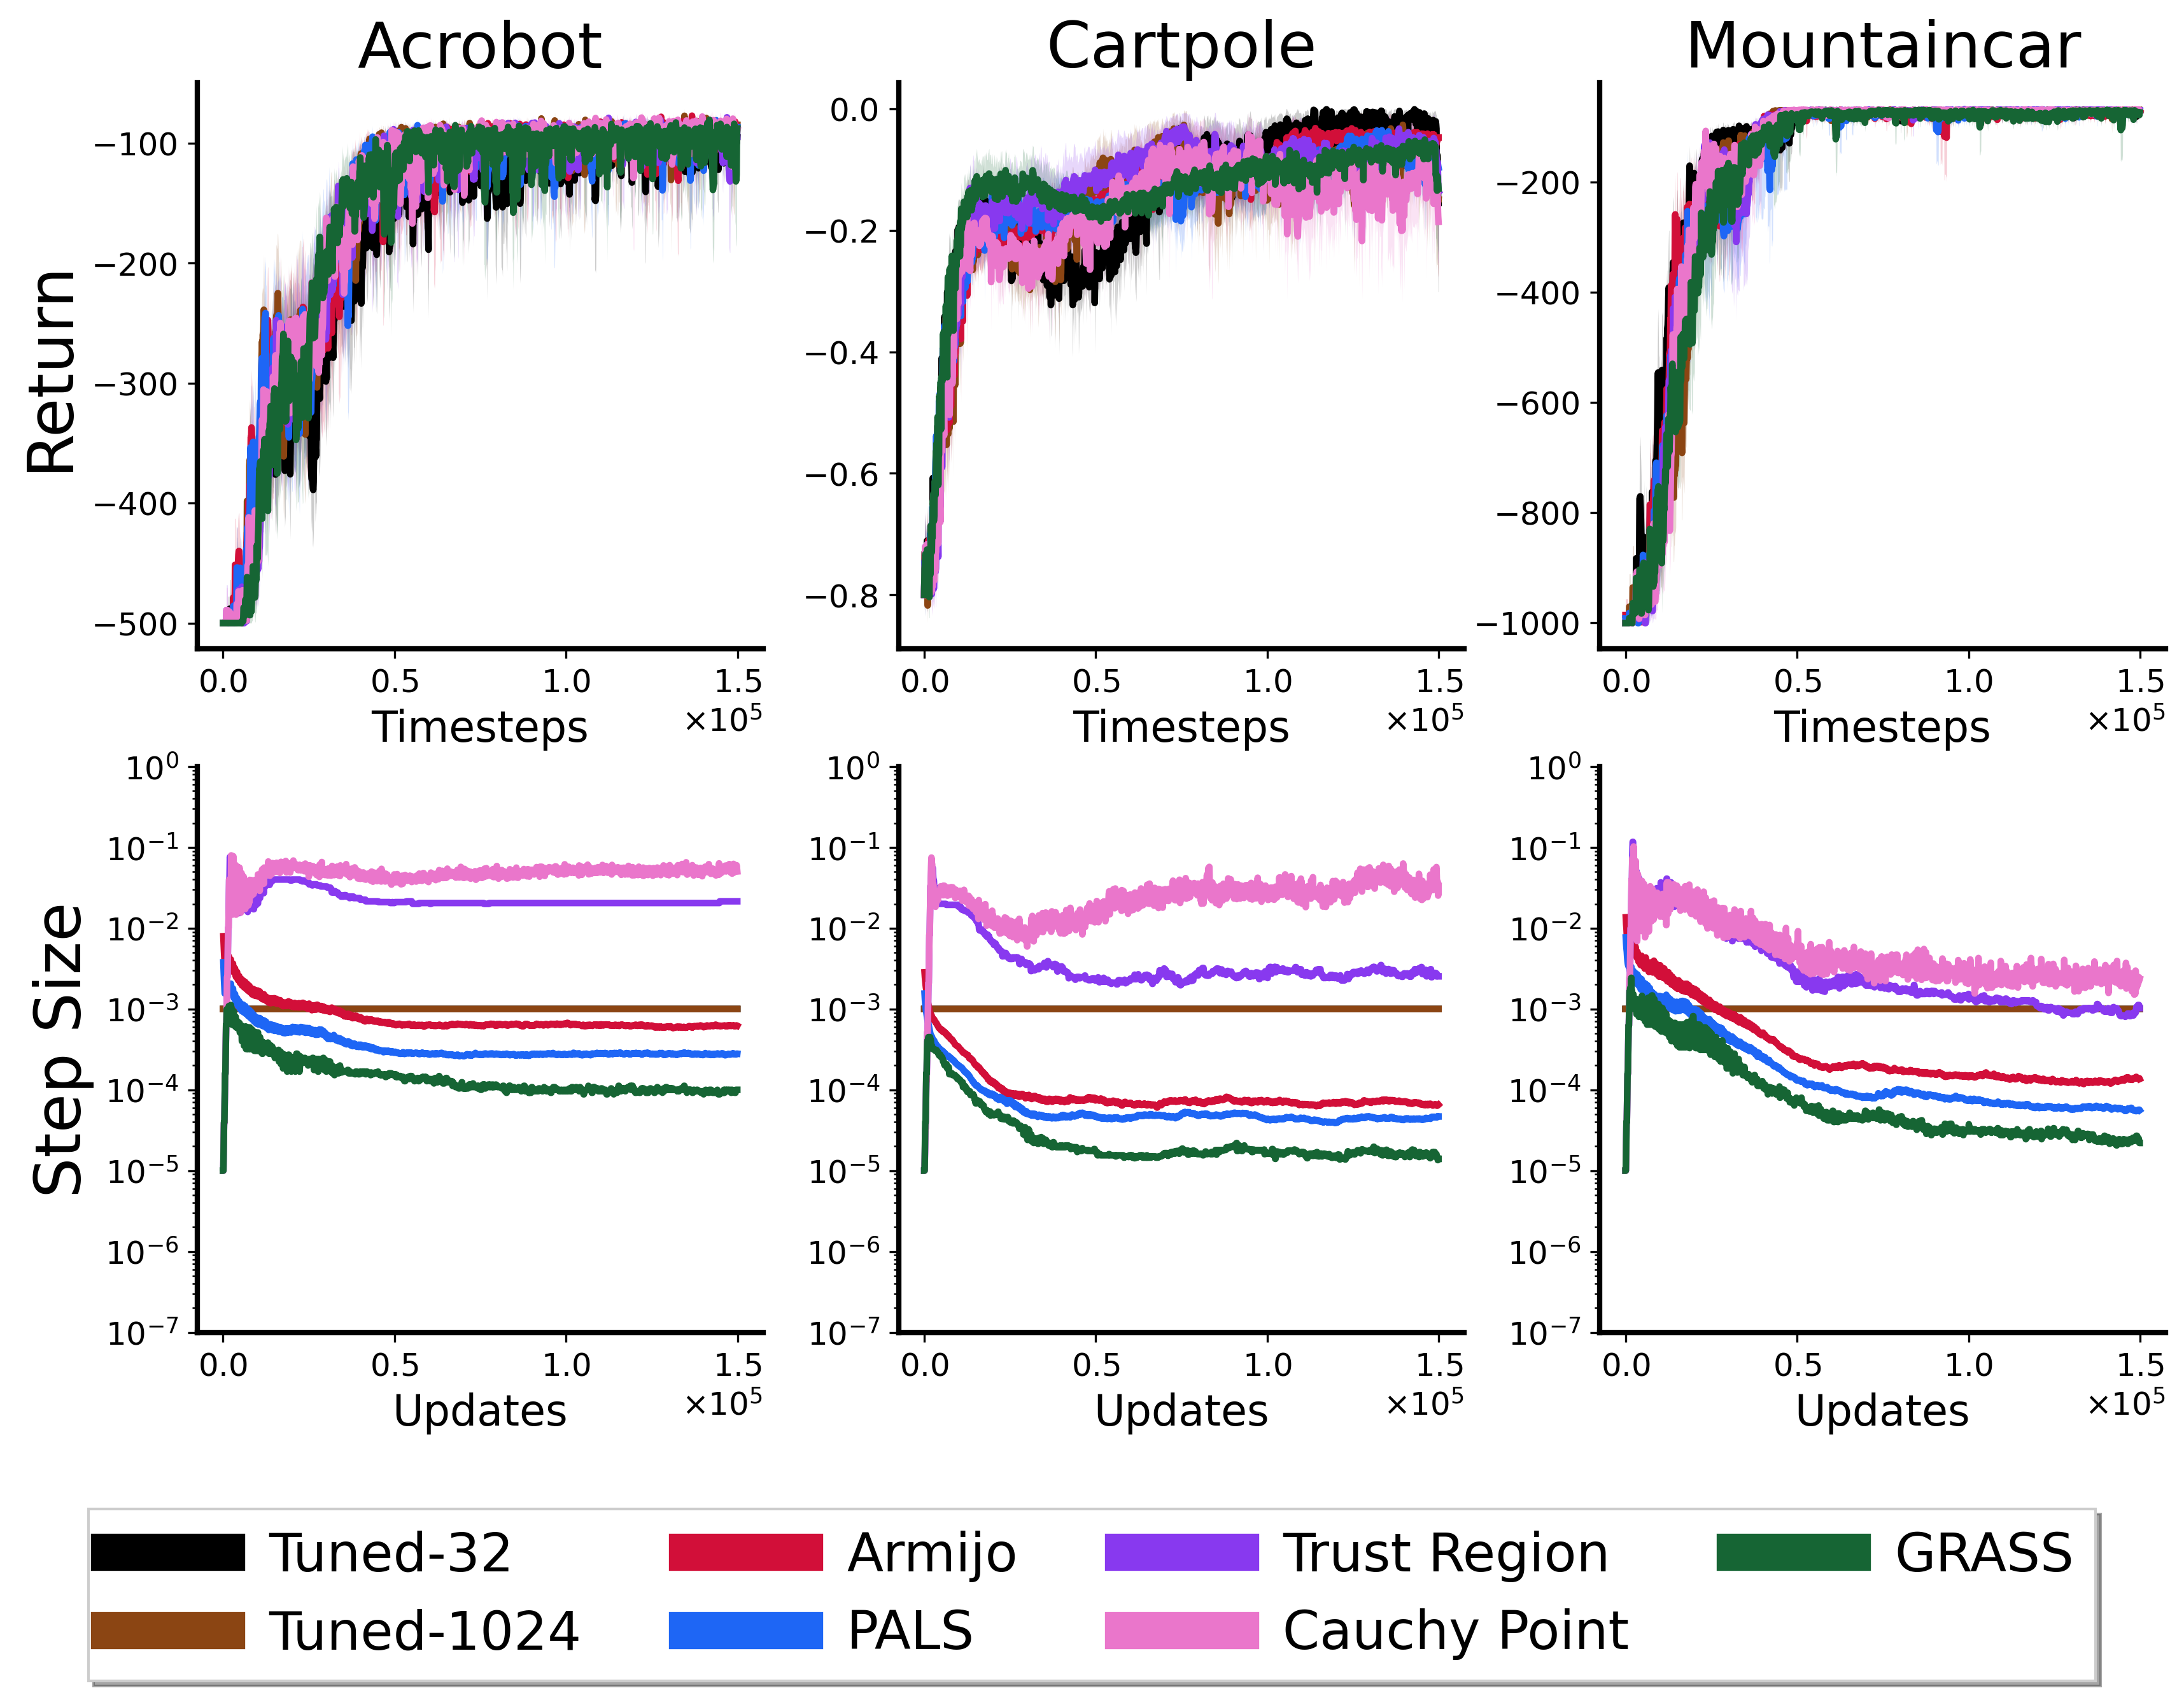
\includegraphics[width=\textwidth]{figures/thesis/performance/1_dqn_classic/dqn_classic_return_step.png}
    \caption[Return and step size for DQN with Adam in classic control.]{Return and step size for DQN with Adam in classic control. All adaptive methods performed roughly equally well across the three environments, matching the tuned baselines.}
    \label{fig:dqn_classic_adam}
\end{figure}

\begin{figure}[htbp]
    \centering
    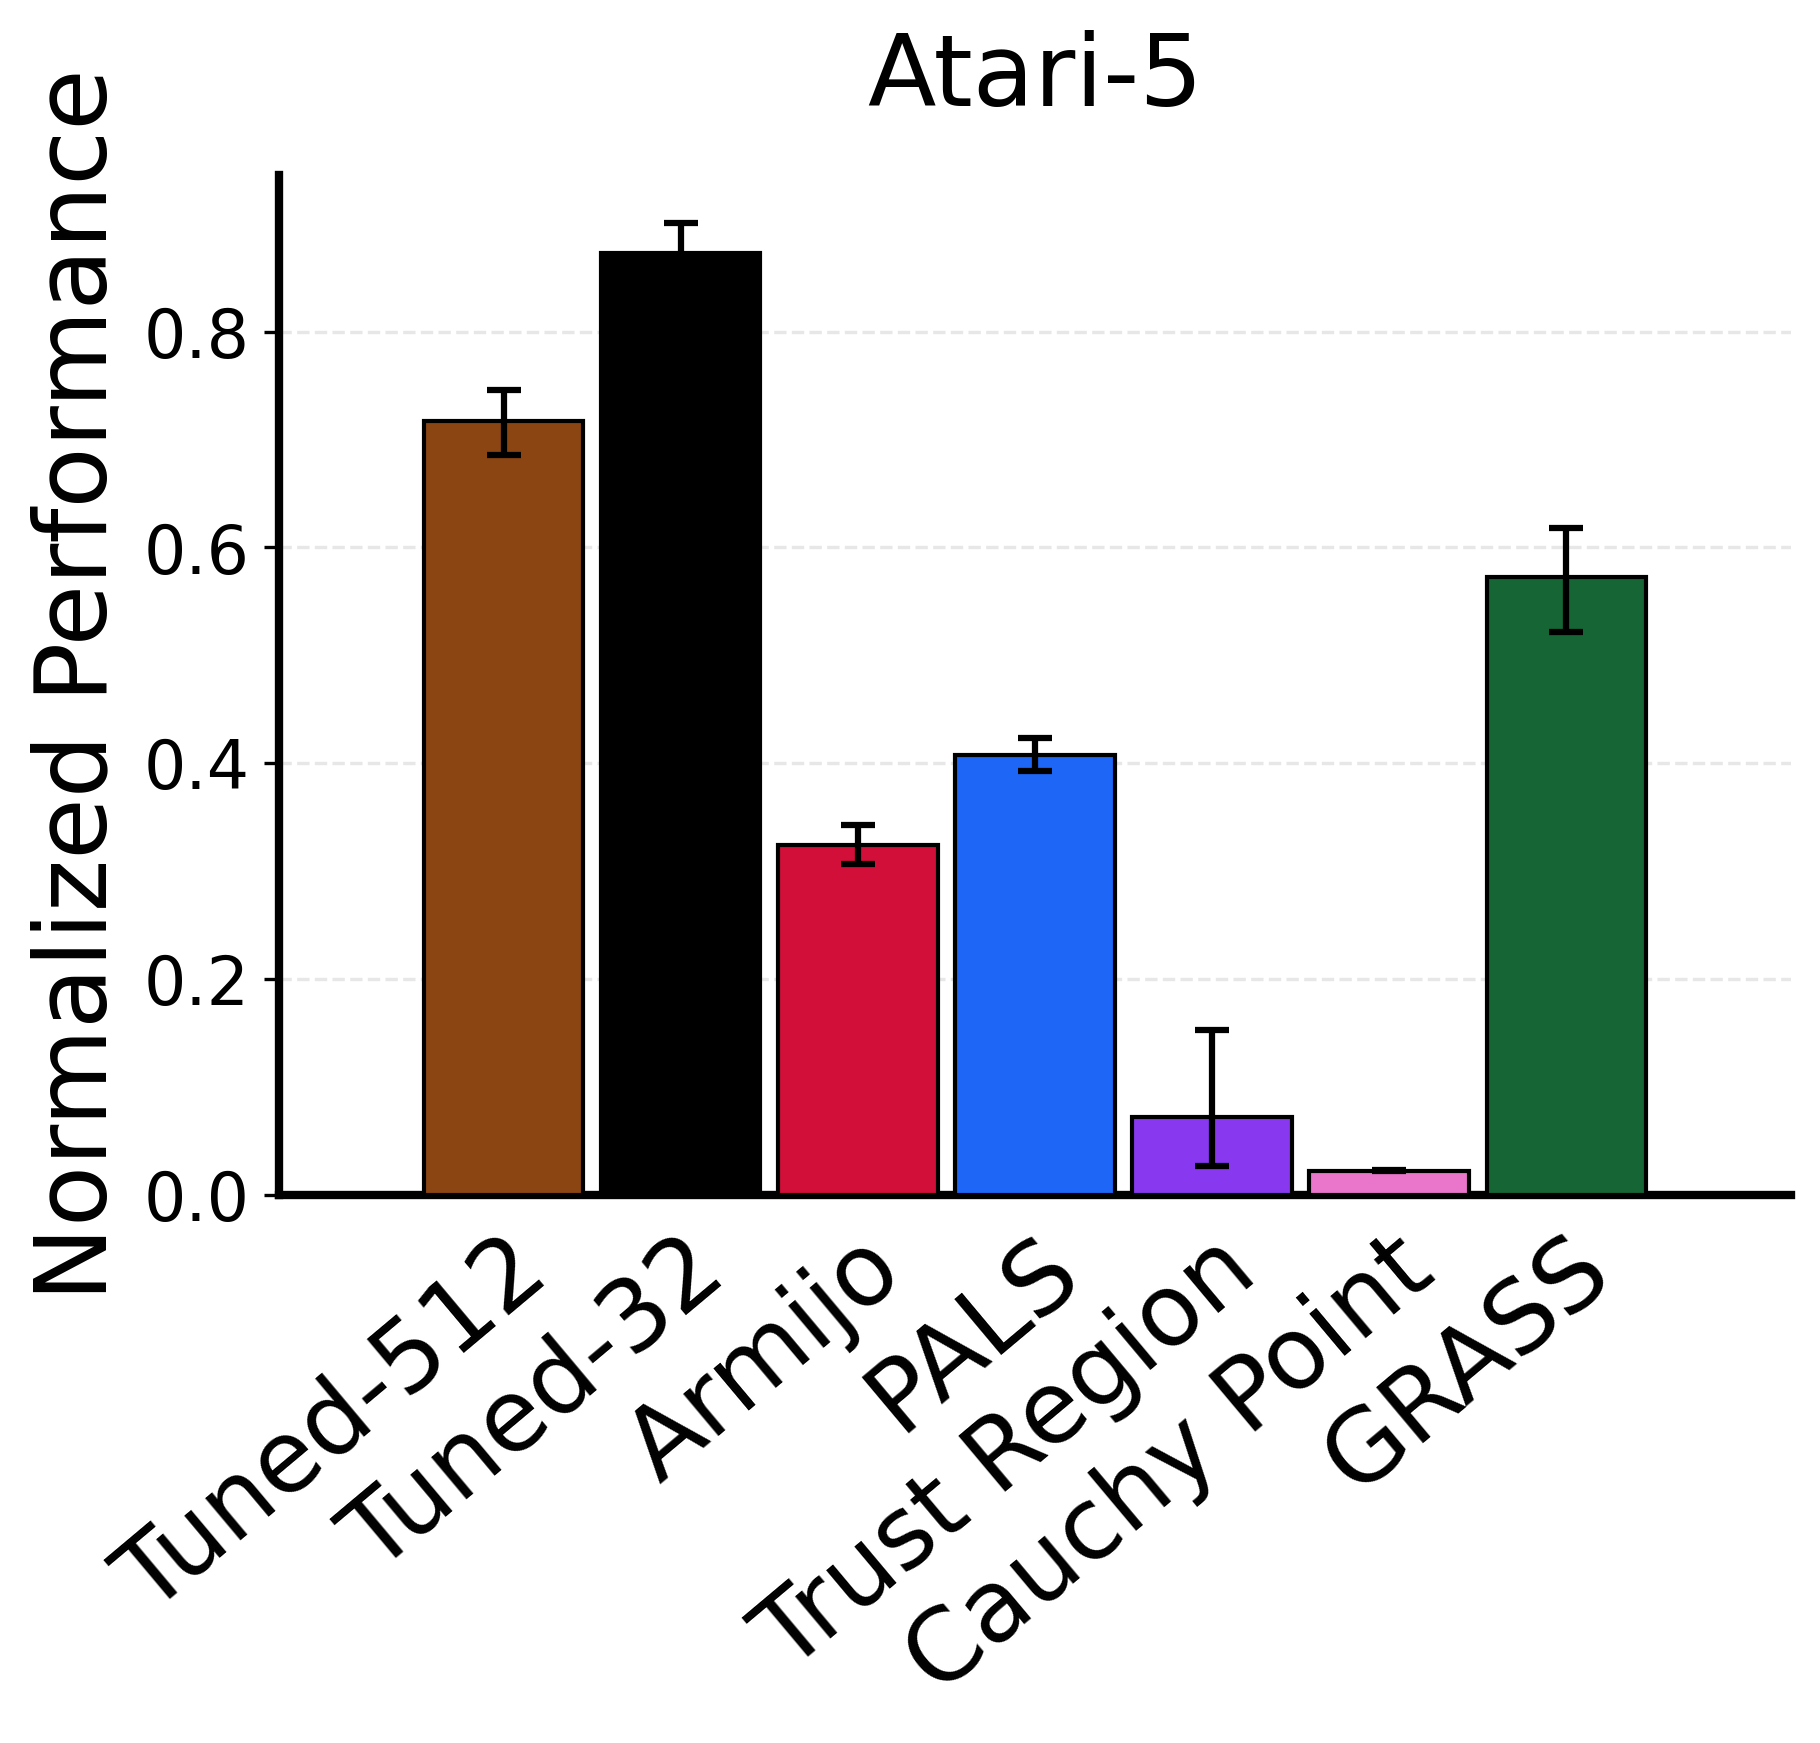
\includegraphics[width=0.45\textwidth]{figures/thesis/performance/2_dqn_atari/dqn_atari_norm_perf.png}
    \caption[Normalized performance of DQN with Adam on the Atari-5.]{Normalized performance of DQN with Adam on the Atari-5. GRASS greatly outperformed the other adaptive methods and surpassed Tuned-512, while PALS matched Tuned-512. Both GRASS and PALS failed to match Tuned-32.}
    \label{fig:dqn_atari_norm_perf}
\end{figure}

Turning to more complex environments, we found the results to be much more nuanced.
Figure~\ref{fig:dqn_atari_norm_perf} shows normalized performance across the Atari-5, where GRASS greatly outperformed all other adaptive step size methods. While GRASS surpassed and PALS matched the Tuned-512 baseline, all other methods did significantly worse. However, both GRASS and PALS still performed worse on average than Tuned-32. Nevertheless, GRASS attained this comparatively strong performance using substantially less compute than the line search methods, as the median gain-ratio requires only two loss evaluations per update rather than the $B+1$ evaluations used by PALS.

Examining the learning curves in Figure~\ref{fig:dqn_atari_adam}, we found that performance in the Atari-5 was much less uniform across methods and environments than in the classic control domains. For example, in Battle Zone, all adaptive methods except GRASS exhibited either a total failure or a clear collapse in return after some period of learning progress. Figure~\ref{fig:dqn_atari_battle_zone} shows these collapses in performance were correlated with steadily increasing step size, loss, gradient norms, and Q-values.

\begin{figure}[htbp]
    \centering
    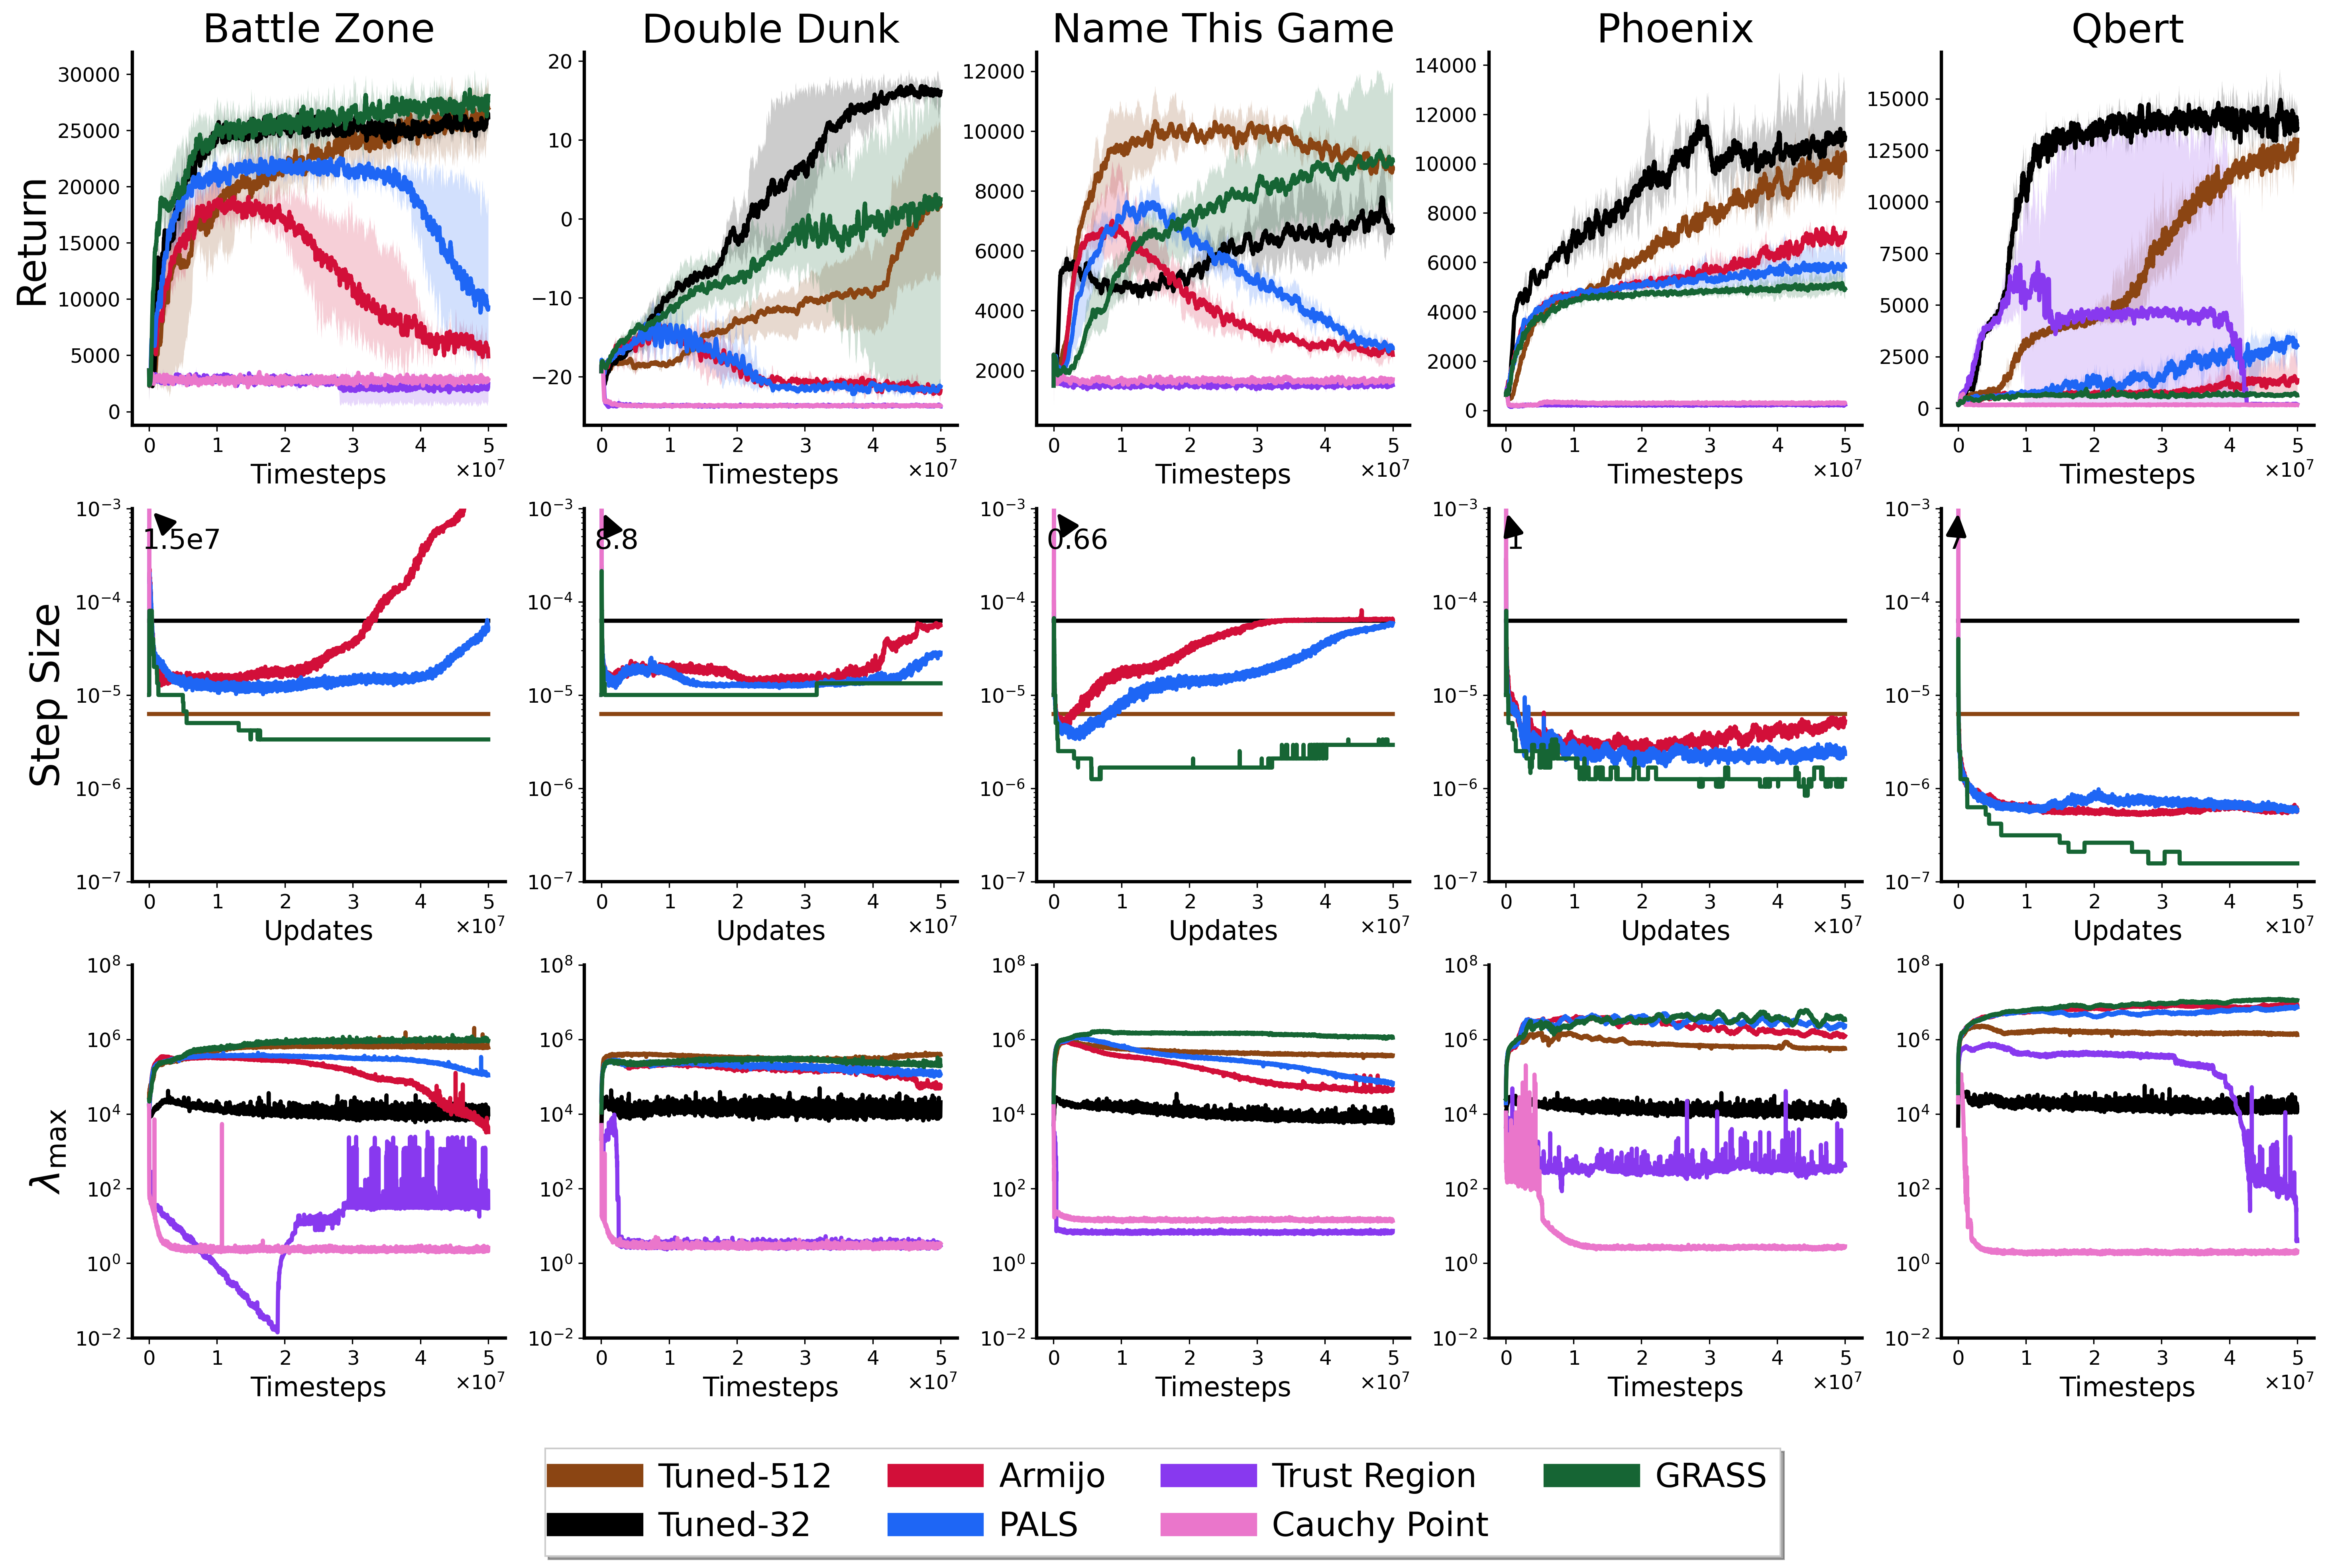
\includegraphics[width=\textwidth]{figures/thesis/performance/2_dqn_atari/dqn_atari_return_step_sharpness.png}
    \caption[Return, step size, and sharpness for DQN with Adam on the Atari-5.]{Return, step size, and preconditioned sharpness $\lambda_{\max}$ for DQN with Adam on the Atari-5. Performance was far less uniform across methods and environments than in classic control, with all adaptive methods except GRASS exhibiting either total failure or a collapse in return in Battle Zone and Name This Game.}
    \label{fig:dqn_atari_adam}
\end{figure}

This finding suggests globalization strategies may be prone to accelerating the instabilities already present under heavy bootstrapping and function approximation. Both the Armijo condition and the gain-ratio only measure whether a step reduced the current objective by a sufficient fraction of the predicted decrease from a local model. Neither method accounts for the fact that larger steps may also inflate the Q-values from which the next targets are formed. Large steps may therefore aggressively generalize and increase the value estimates used to compute the new targets at the next refresh. The steady growth in the value estimates is consistent with such a loop, however it may also hold that step sizes selected based on the batch loss simply exceed those which the true loss supports. Additionally, early in learning the bootstrapped targets are largely based on randomly initialized values, and therefore aggressively minimizing the loss could be harmful at this stage. Lastly, we did not re-tune any of DQN's other hyperparameters when using globalization strategies in place of a fixed step size, which may result in instabilities, as DQN is notoriously sensitive to its hyperparameters \todo{Citation}.

\begin{figure}[htbp]
    \centering
    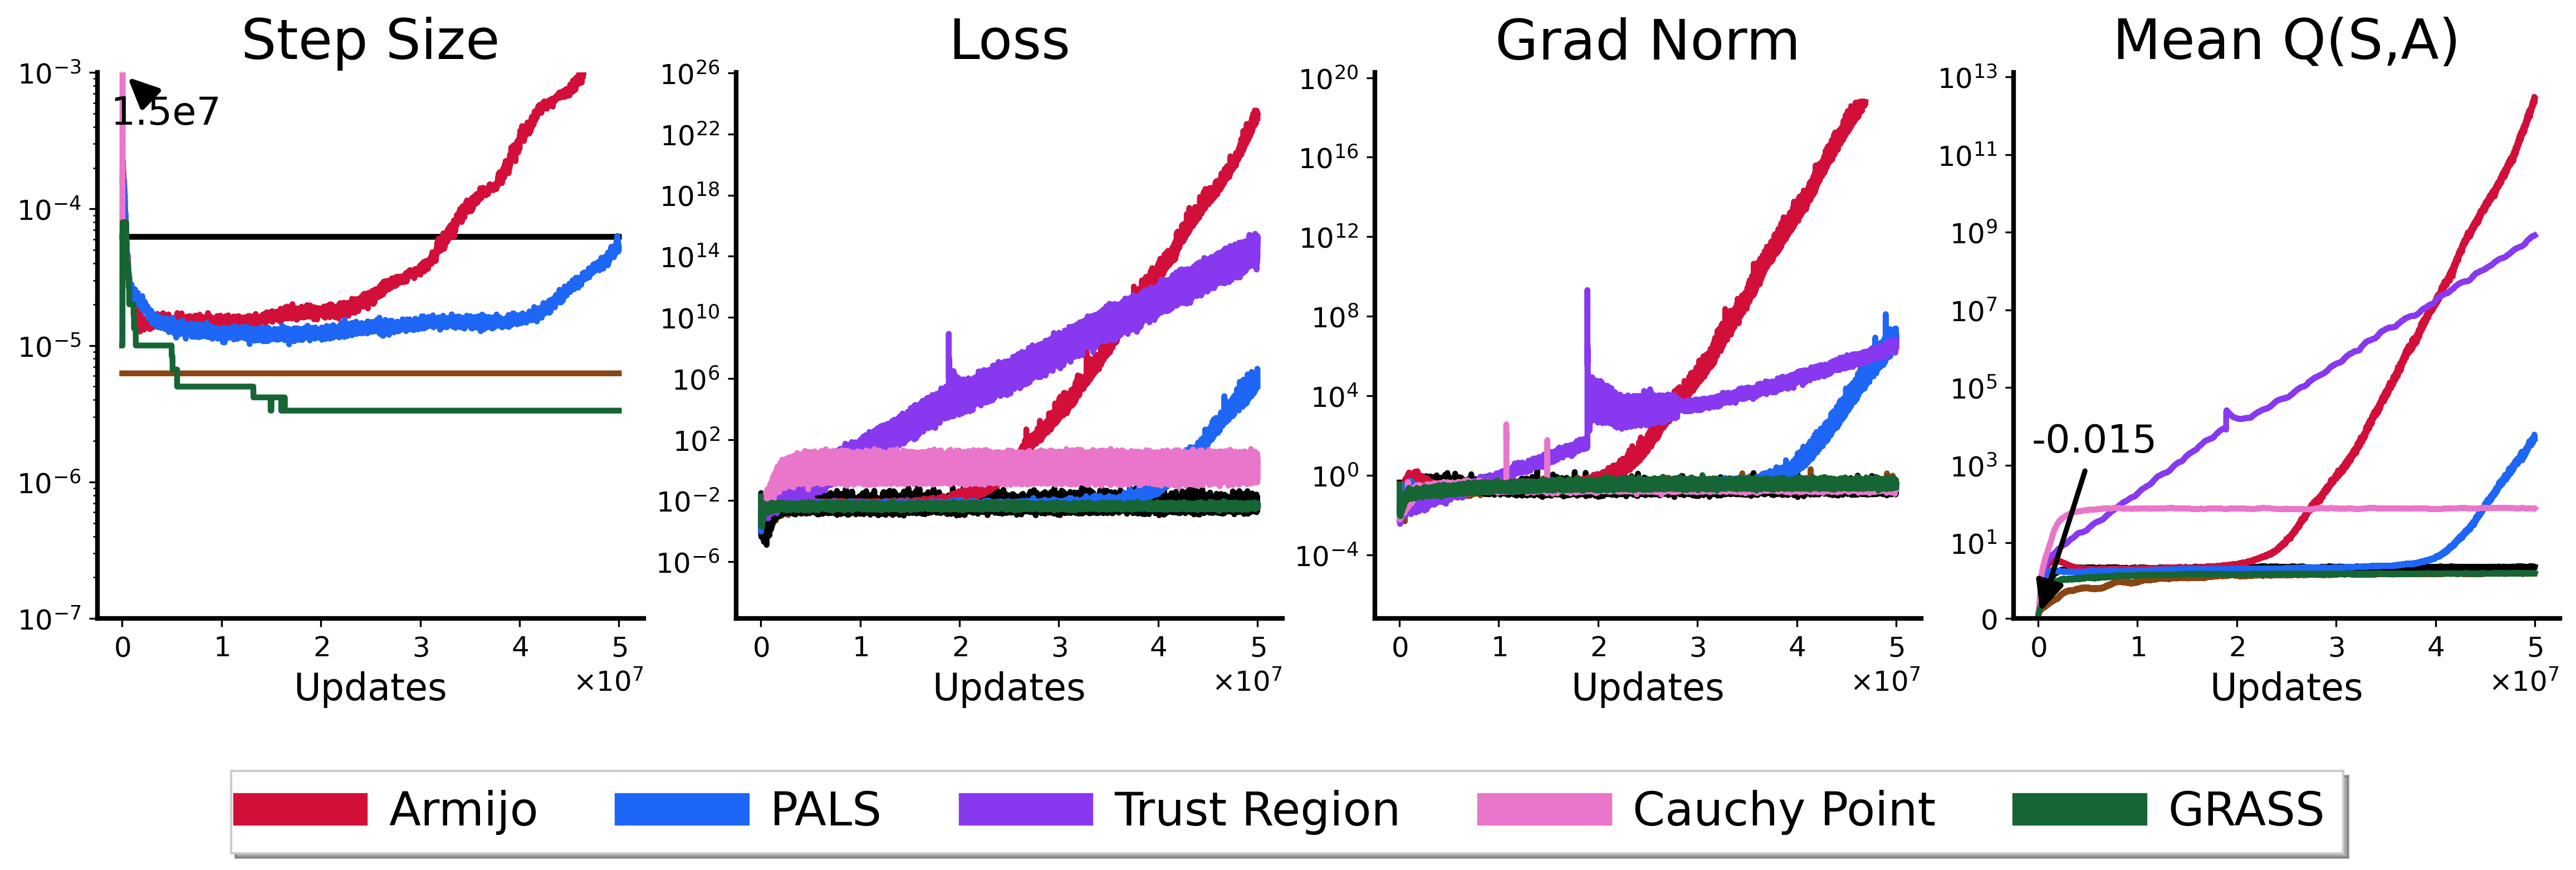
\includegraphics[width=\textwidth]{figures/thesis/performance/2_dqn_atari/dqn_atari_battle_zone_metrics.png}
    \caption[Return, step size, loss, gradient norm, and Q-values for DQN in Battle Zone.]{Return, step size, loss, gradient norm, and Q-values for DQN with Adam in Battle Zone. The collapse in return for all adaptive methods except GRASS was correlated with steadily increasing step size, loss, gradient norms, and Q-values.}
    \label{fig:dqn_atari_battle_zone}
\end{figure}

GRASS may be less afflicted by the feedback loop described above because its chosen step size stabilizes much earlier in the run as compared to the other adaptive methods. Because $\stepSize$ scales a unit vector rather than the raw update with standard trust region methods, the displacement per update is $\stepSize$ rather than $\stepSize \norm{\updateAt{k}}$. Starting from the same $\trustRegionInit$ of $1e-5$, we observed an initial growth period for both GRASS and the trust-region methods. However, for GRASS the median gain-ratio quickly fell below $T_{\text{hi}}$ and the step size then shrank accordingly. Since the effective displacement is smaller by a factor of $\norm{\updateAt{k}}$ for trust region methods, their step size continued to grow. Similarly, unlike GRASS, the examined line search methods adjust the step size each update and always consider the maximum step of $1$, making them more prone to the same divergent behavior. \todo{Q for Adam: not sure if this makes sense re regular TR being more susceptible to divergence bc there are more updates with larger ss early on}

% Interestingly, this phenomenon is not observed in Name This Game. As shown in % todo: ref appendix with dqn atari curves
% we again observe decline in return correlated with increasing step sizes, however there is no corresponding trend in the loss, TD-error, gradient norms or Q-values, all of which are indistinguishable from the tuned baselines. However, the decline again appears to be a consequence of the larger batch size. Recall that Tuned-32 and Tuned-512 use an identical step size of $6.25\mathrm{e}{-5}$, and we observe that Tuned-512 performs much worse than Tuned-32 in this environment. Over the course of the run, Armijo and PALS raise their step sizes from roughly $5\mathrm{e}{-6}$ to approximately this value, and their return decays from a peak above Tuned-32 down to the level of Tuned-512. Rather than failing by diverging, these methods gradually settle on a step size that clearly performs poorly at their batch size, and performance declines accordingly. By contrast, GRASS, which selects step sizes roughly 1000 times smaller, achieves the best performance in this environment. 
% This failure mode again appears to be a consequence of the dependence of globalization methods on large batch size in RL control examined in Section~\ref{sec:batch_size}, in tandem with the sensitivity of the DQN algorithm to batch size. 
% That GRASS is again the exception follows from how conservative it is by construction. The Armijo condition with sufficient decrease constant $c$ is exactly the requirement $\rho_k \ge c$, so with $c = 0.1$ the line search methods accept any step realizing a tenth of the predicted decrease on the current batch. GRASS instead requires a median gain-ratio above $T_{\text{hi}} = 0.75$ over a window of $K$ updates before increasing $\stepSize$, and shrinks $\stepSize$ whenever that median falls below $T_{\text{lo}} = 0.25$. It is therefore stricter about what counts as an accurate step, and less exposed to the variance of any individual batch.

% ---------------------------------------------------------------------------
% ALTERNATIVE ACCOUNT OF NAME THIS GAME (opus, per your note). Swap in for the
% paragraph above if you prefer it. The two are mutually exclusive.
%
% A simpler account of this environment is available. The step size selected by
% the grid search at batch size $512$ was the smallest value in the range tested
% (Appendix~\ref{app_tuning_ranges}), so the best fixed step size at this batch
% size is plausibly lower still, and $6.25\mathrm{e}{-5}$ should be read as an
% upper bound rather than an optimum. Under this reading nothing pathological
% occurs in Name This Game. The step size appropriate to batch size $512$ is
% simply much smaller than the one appropriate to batch size $32$, and Armijo
% and PALS climb past it. The Armijo condition with sufficient decrease constant
% $c$ is exactly the requirement $\rho_k \ge c$, so with $c = 0.1$ a step is
% accepted whenever it realizes a tenth of the predicted decrease on the current
% batch. This continues to hold well past the step size that is good for
% learning, as a step can reduce the loss on the batch it was computed from
% while still being too large for the objective the agent is optimizing. GRASS
% avoids the problem because it requires a median gain-ratio above
% $T_{\text{hi}} = 0.75$ over a window of $K$ updates before increasing
% $\stepSize$, and shrinks $\stepSize$ whenever that median falls below
% $T_{\text{lo}} = 0.25$.
% ---------------------------------------------------------------------------

Unlike in Battle Zone, returning to Figure~\ref{fig:dqn_atari_adam}, we observed that for Qbert, step sizes were roughly $10^2$ to $10^4$ times smaller than the tuned baselines, and roughly 10 to 100 times smaller than the chosen step sizes in the other Atari environments. All adaptive methods performed poorly in this environment, and we found that performance was correlated with sharpness in the loss, with GRASS and both line search methods reaching preconditioned sharpness roughly 1000 times greater than the baselines.

Step size and sharpness are inherently tied, as the EOS literature has shown that in non-convex optimization, parameters settle at a sharpness inversely proportional to the step size. While the adaptive methods operated in sharper regions of parameter space than the tuned baselines in all five environments, the pattern was most extreme in Qbert, where they also performed the worst overall. This finding is aligned with the failure mode reported for line search methods in full-batch supervised learning \cite{roulet2024stepping}, where they selected overly conservative step sizes and failed to reach the EOS. Additionally, we observed that sharpness for the baseline methods in all Atari environments appeared to converge to roughly $2/\eta$, as observed for RMSProp in supervised learning \tocite{citation}. Yet, interestingly, these methods utilize the Adam optimizer, for which convergence to $38/\eta$ is expected \tocite{citation}.

These findings demonstrate that several unique failure modes exist for globalization strategies in deep RL, which may result in both overly conservative and aggressive step sizes depending on the environment. Nevertheless, the strong performance of GRASS relative to Tuned-512 and competitive performance with Tuned-32 in $3/5$ environments suggests that it remains a promising approach for adaptive step size with DQN. 
\section{Adaptive Step Size with PPO}
\begin{figure}[htbp]
    \centering
    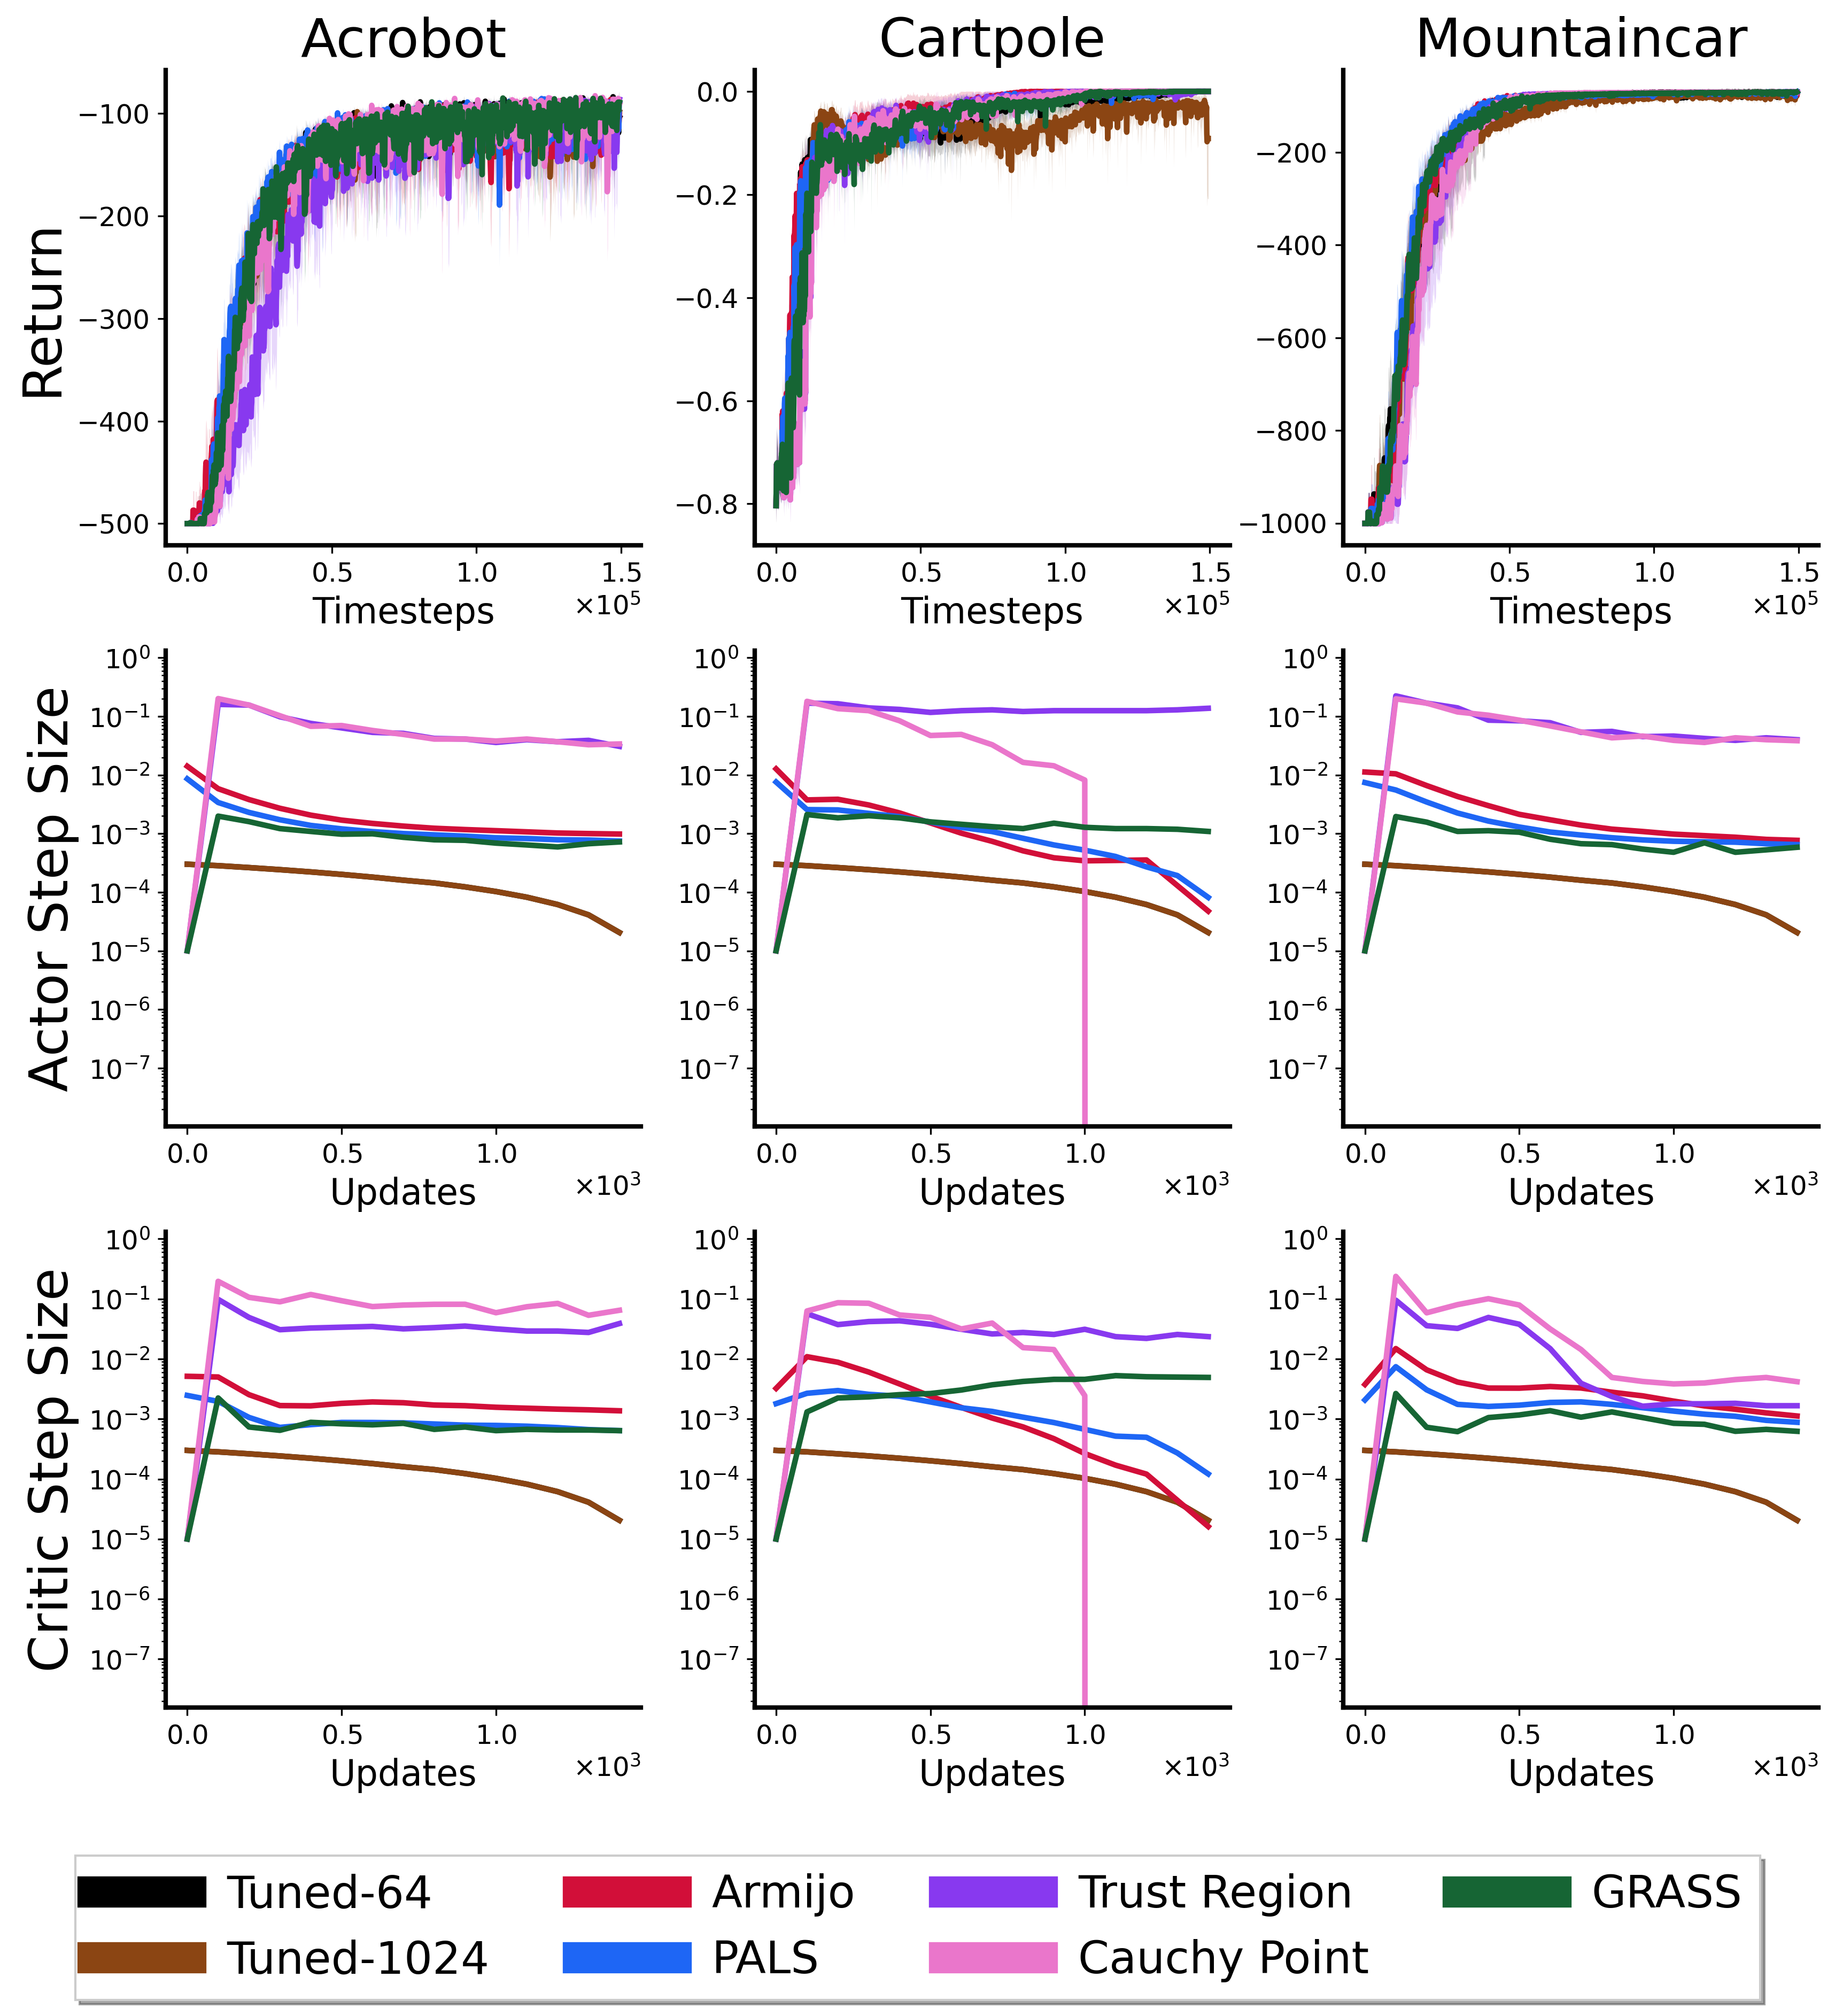
\includegraphics[width=\textwidth]{figures/thesis/performance/3_ppo_classic/ppo_classic_return_step.png}
    \caption[Return and step size for PPO with Adam in classic control.]{Return and step size for PPO with Adam in classic control. All methods performed roughly equally well, matching the tuned baselines.}
    \label{fig:ppo_classic_adam}
\end{figure}
\begin{wrapfigure}{R}{0.47\textwidth}
    \centering
    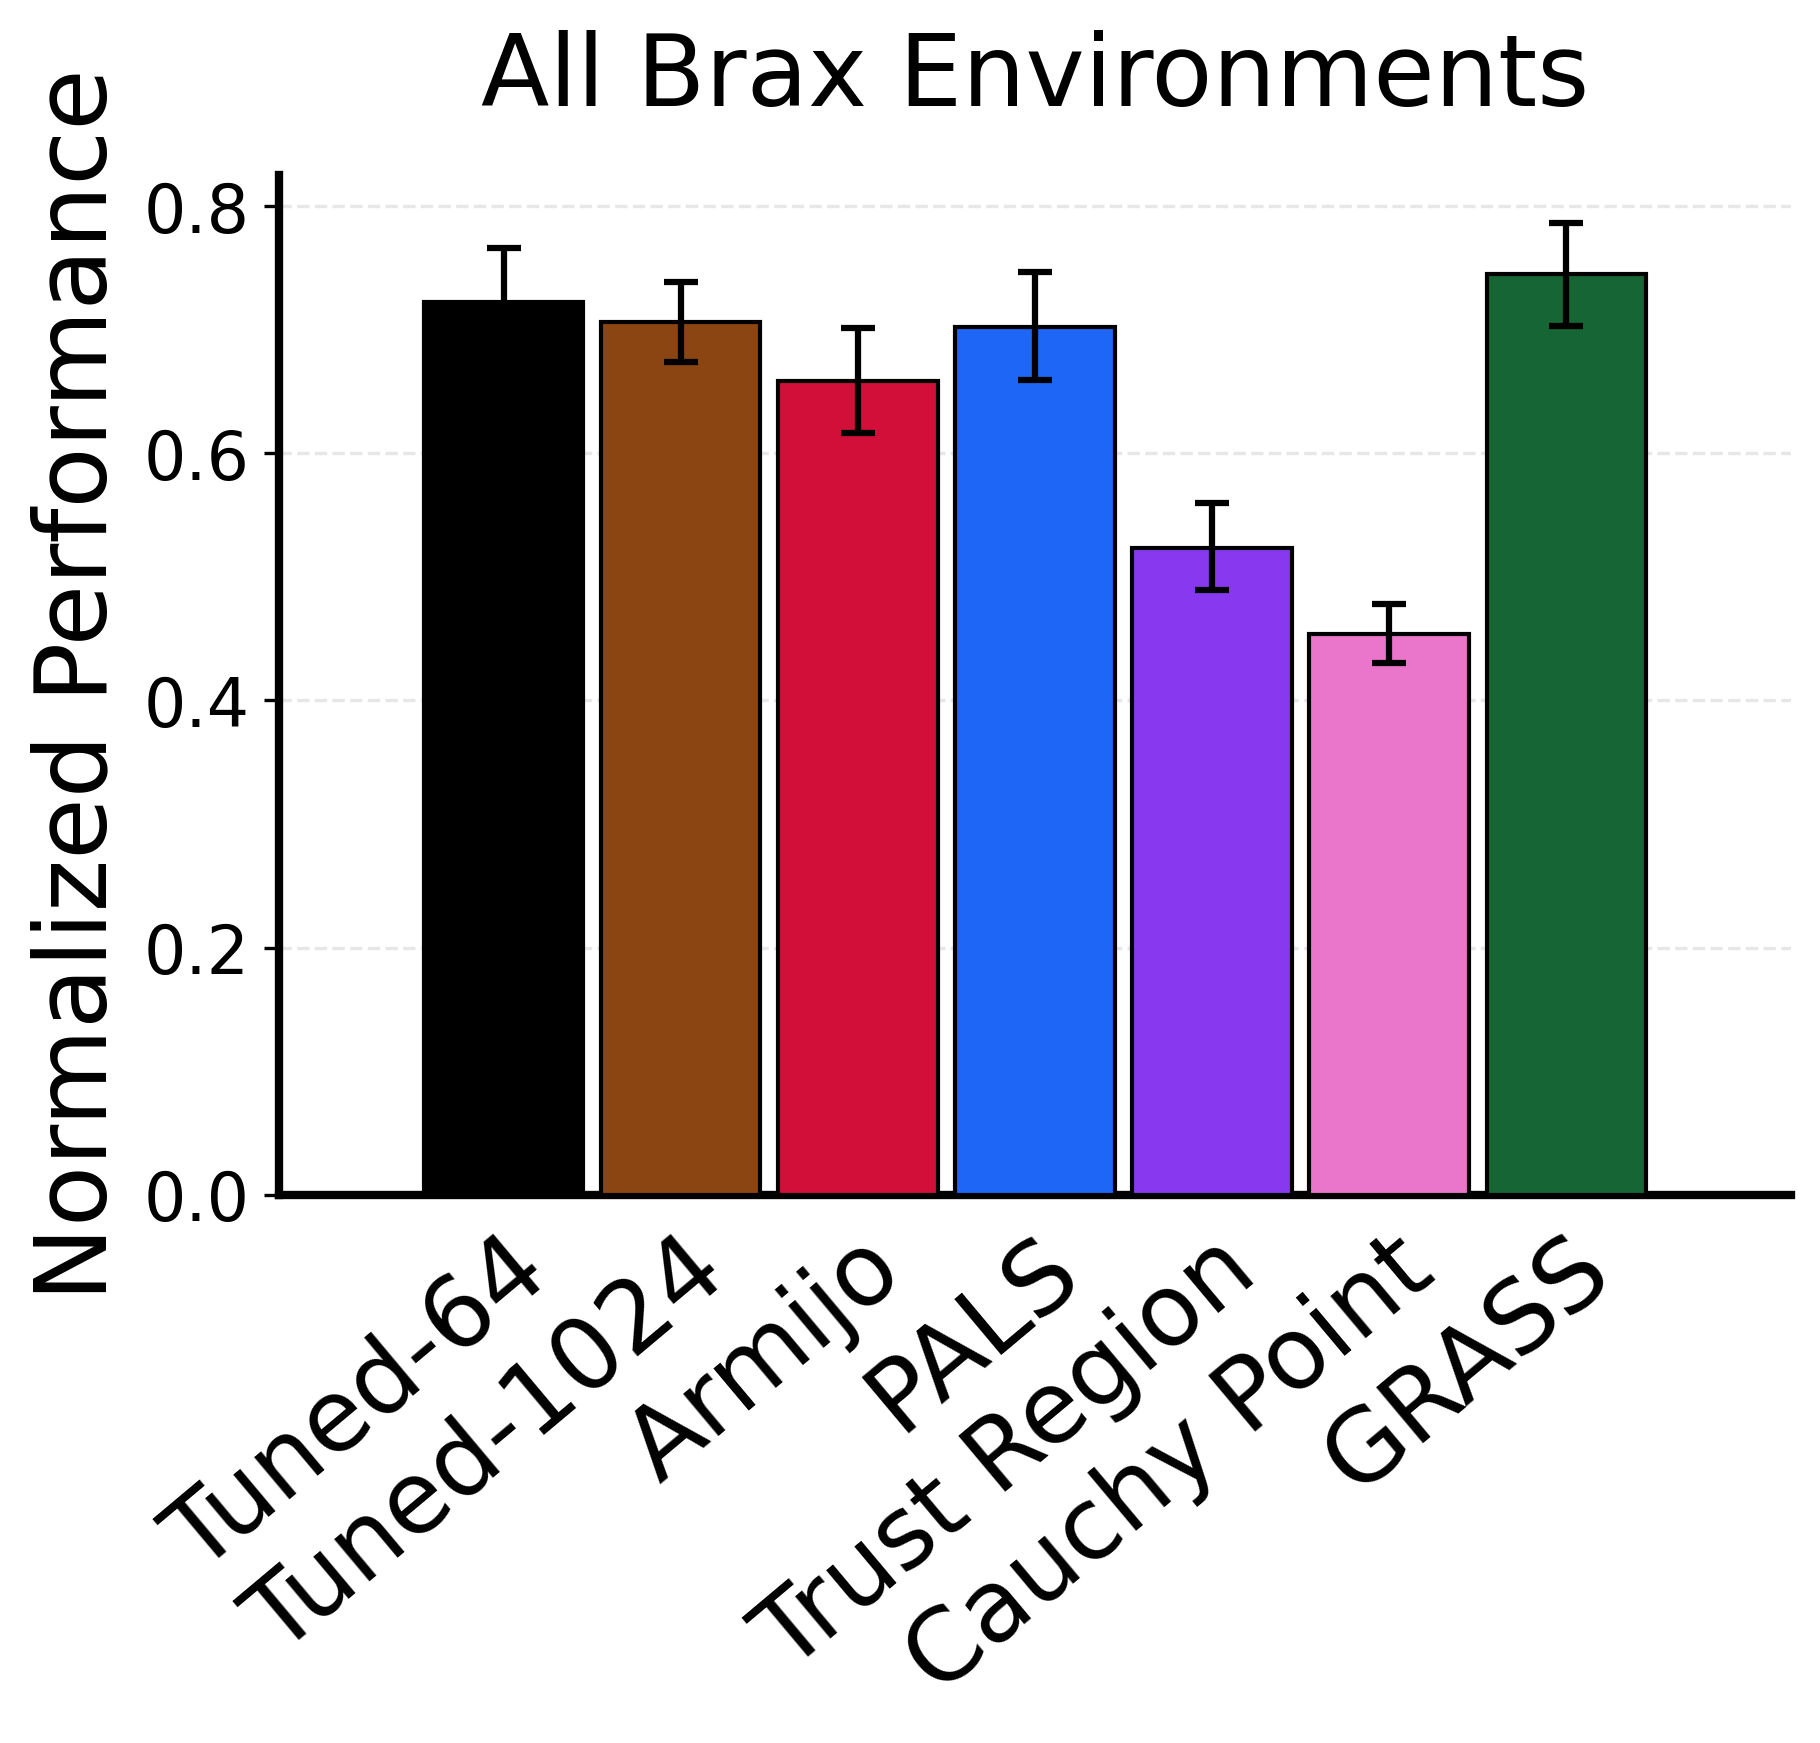
\includegraphics[width=0.45\textwidth]{figures/thesis/performance/4_ppo_mujoco/ppo_mujoco_norm_perf.png}
    \caption[Normalized performance of PPO with Adam on Brax.]{Normalized performance of PPO with Adam on Brax. GRASS and PALS performed on par with the tuned baselines, while the standard Trust Region methods performed worse.}
    \label{fig:ppo_mujoco_norm_perf}
\end{wrapfigure}
We now examine adaptive step size for PPO, beginning with the classic control suite. Similarly to DQN, Figure~\ref{fig:ppo_classic_adam} shows that all methods performed roughly equally well, matching the tuned baselines. Chosen step sizes for line search methods and GRASS lay roughly within an order of magnitude above the tuned step size, while those of standard trust region methods were higher, as they normalize the update vector.

Moving to Brax, Figure~\ref{fig:ppo_mujoco_norm_perf} shows that GRASS and PALS performed on par with the tuned baselines across the suite. Backtracking Armijo nearly matched the baselines, while the standard trust region methods performed worse. Examining the learning curves in Figure~\ref{fig:ppo_mujoco_adam}, we found that GRASS and PALS were consistently competitive with the best tuned baseline in $4/5$ environments, while the backtracking Armijo and Trust Region methods sometimes performed much worse than the fixed-schedule baselines. Additionally, Tuned-64 achieved higher return than Tuned-1024 in $4/5$ environments, yet reached less than a third of its return in Humanoid. No fixed pairing of step size and batch size is therefore reliable across the whole suite. Note that we never observed a failure of this magnitude for GRASS or PALS, demonstrating that the benefit of adaptive step size selection in this setting is primarily reliability across environments rather than a large gain in any individual environment.

\begin{figure}[htbp]
    \centering
    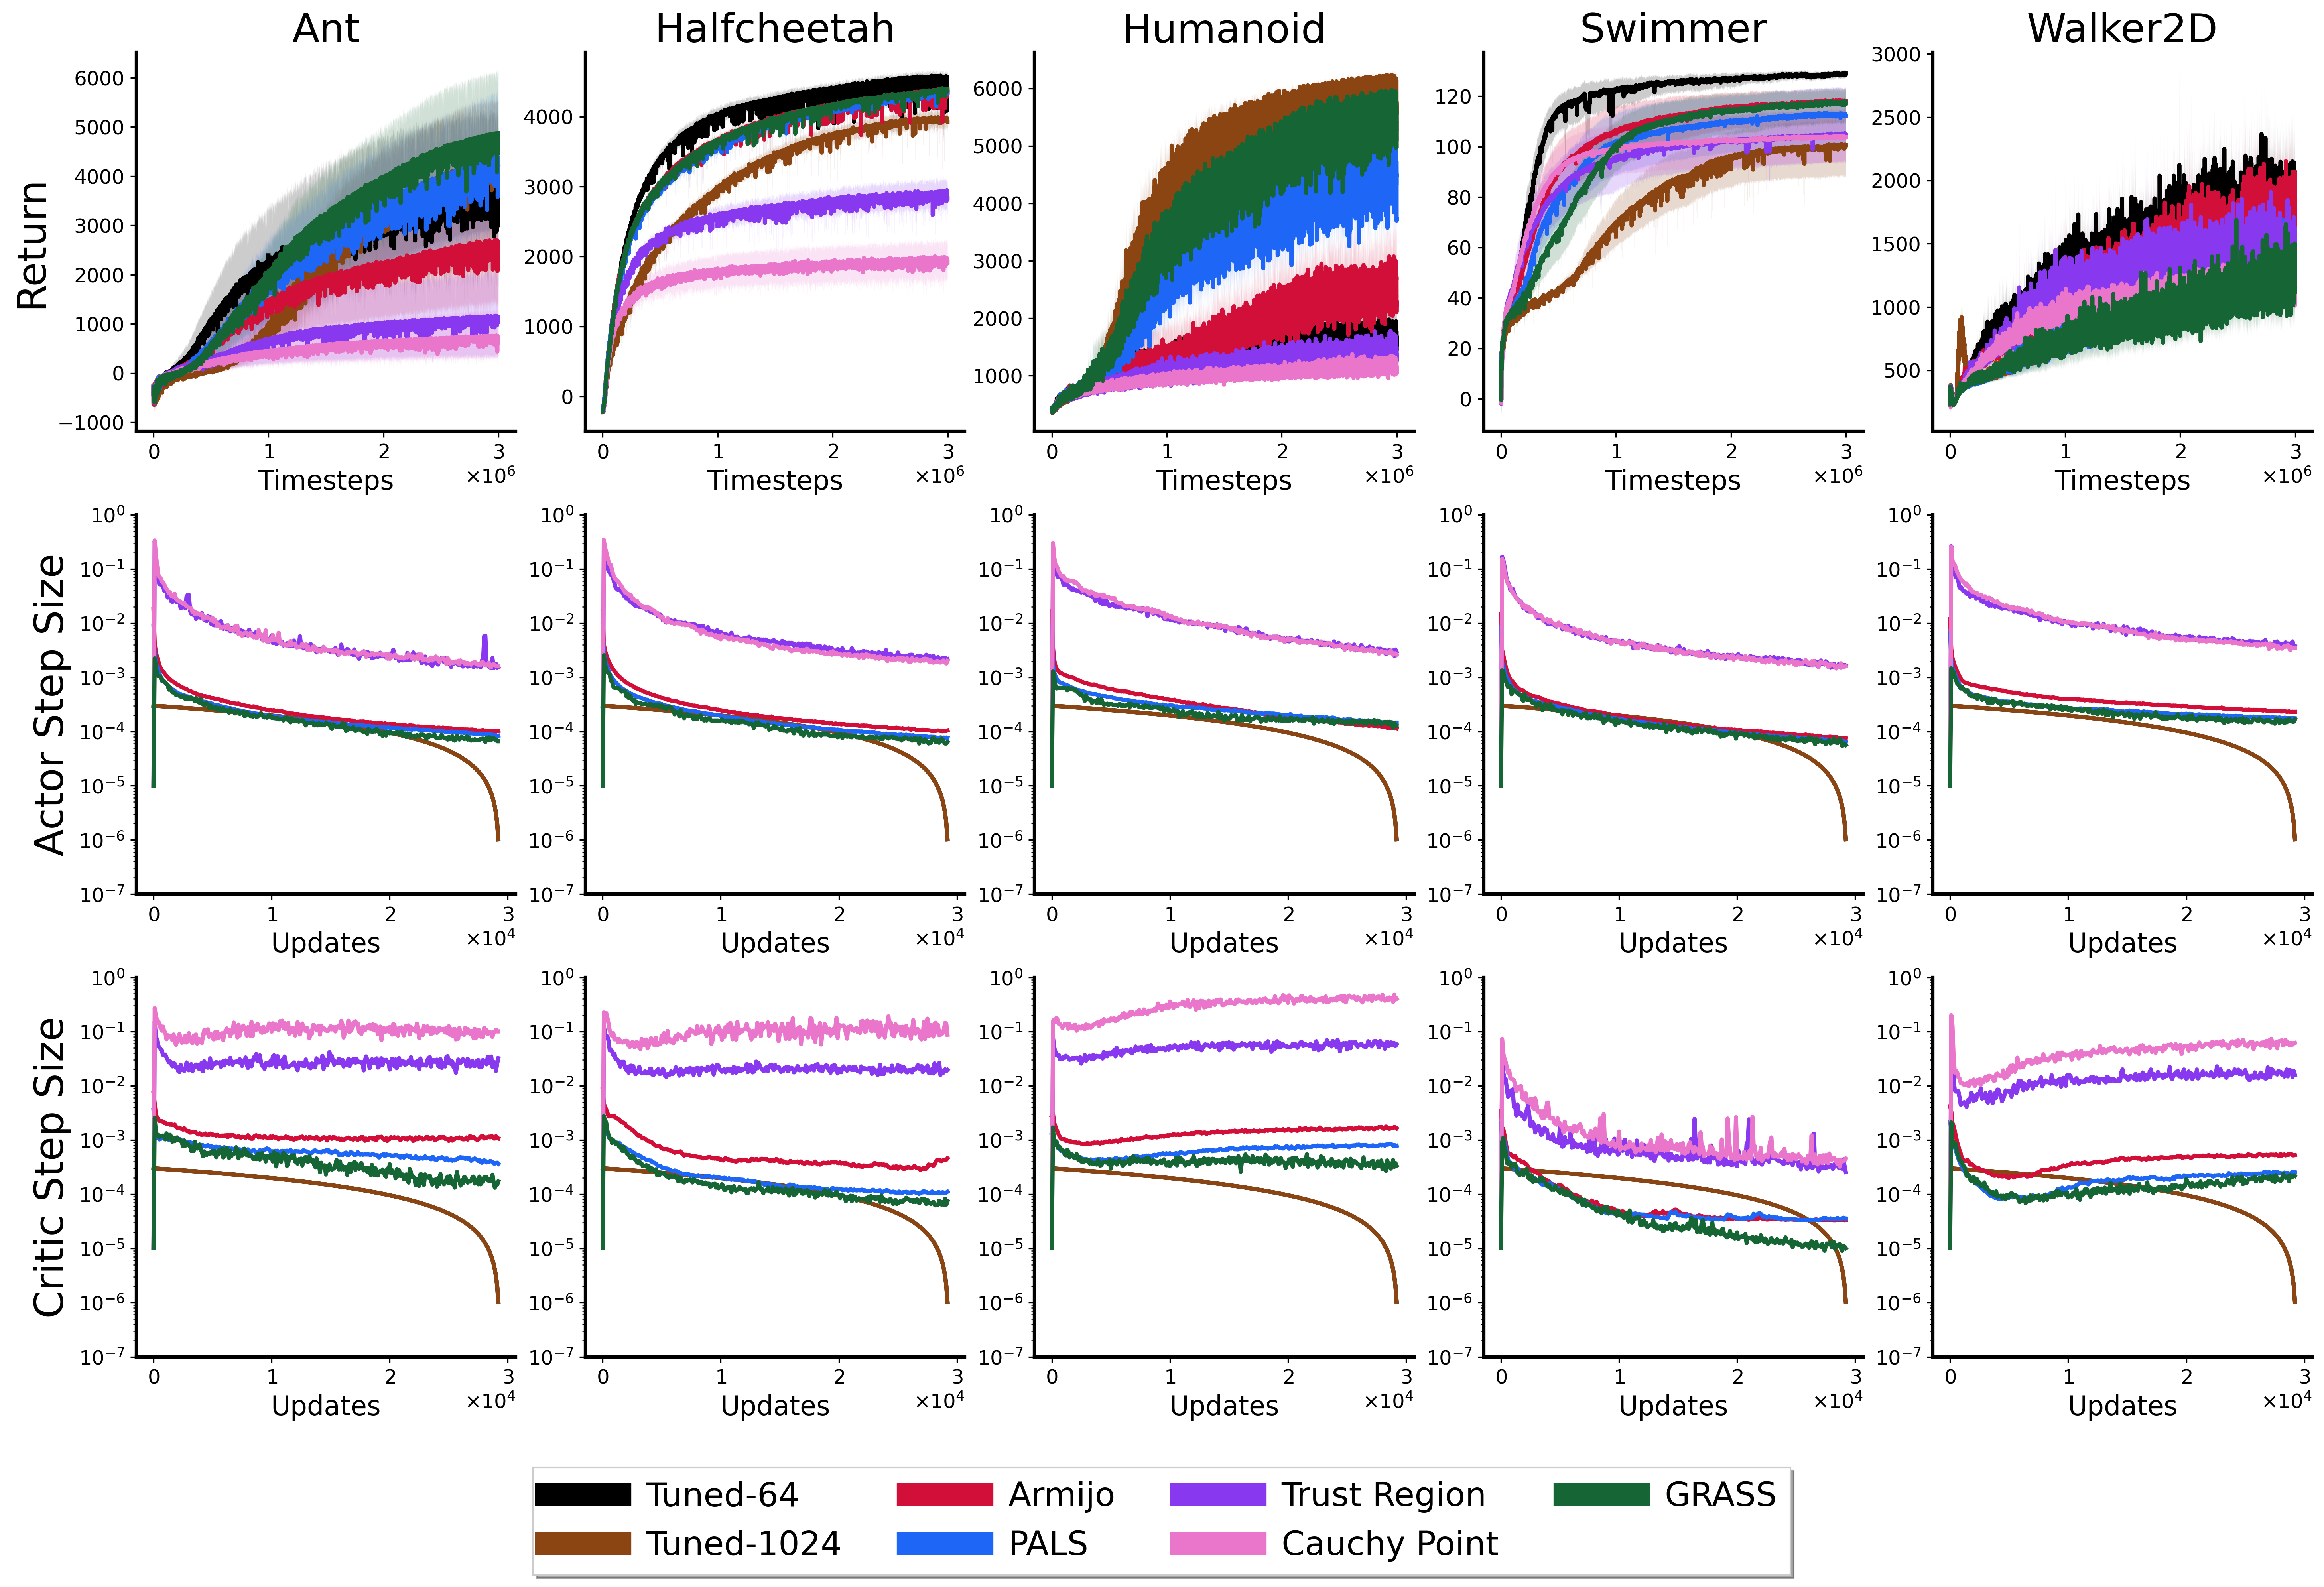
\includegraphics[width=\textwidth]{figures/thesis/performance/4_ppo_mujoco/ppo_mujoco_return_step.png}
    \caption[Return and step size for PPO with Adam in Brax.]{Return and step size for PPO with Adam in Brax. GRASS and PALS were competitive with the best tuned baseline in $4/5$ environments, while the backtracking Armijo and Trust Region methods sometimes performed much worse than the fixed-schedule baselines.}
    \label{fig:ppo_mujoco_adam}
\end{figure}

As with DQN, Figure~\ref{fig:ppo_mujoco_adam} shows that GRASS and line search methods fell within an order of magnitude of the baseline while the Trust Region methods had larger step sizes. Notably, no methods exhibited either the divergent or the overly conservative step sizes observed in some Atari environments with DQN. We hypothesize this is primarily due to using PPO rather than a product of the Brax environments, for several reasons. First, unlike the single-step Q-learning loss used by DQN, the critic targets in PPO are computed using $\lambda$-returns, which place most of their weight on observed rewards rather than the value estimates produced by the preceding update phase. This may alleviate the hypothesized instabilities related to single-step targets discussed in Section~\ref{sec:dqn_results}. The critic target also involves no maximization over actions, so it does not contain the inherent upward bias that can result in overestimation with DQN \todo{cite double q paper}. Additonally, the buffer of $2048$ transitions collected by PPO is likely more on-policy than the large replay buffer of $1,000,000$ transitions maintained by DQN, suggesting that interpolation condition in % todo: ref background section for line search and trust region
may be more likely to hold. % todo: does this make sense? that being more on-policy means interpolation is likely to hold because the loss in rl is always defined over the on-policy distribution? 
Lastly, once the likelihood ratio in the policy loss leaves the clipping range, the surrogate objective becomes flat along that direction. As a result, larger steps yields no further improvement, directly capping the step size these methods will accept for the actor. 
% As more of a minibatch has its importance ratio pushed outside $[1 - \epsilon, 1 + \epsilon]$, moving further along the update direction yields less and less additional decrease. Oversized actor steps are therefore caught by the selection criteria themselves, as the realized decrease falls short of the decrease predicted by the local model.
The comparatively lower-dimensional proprioceptive observations in Brax also likely pose a better conditioned optimization problem than learning from raw pixels, though our experiments do not fully isolate this factor from the choice of algorithm.

The superior performance of GRASS relative to the Trust Region methods in this setting suggests that preserving the magnitude of the update, rather than using only its direction, is especially useful in these environments. While the displacement in parameter space for GRASS is proportional to the magnitude of the raw update vector, traditional trust region methods are not affected by this quantity and can only adjust the displacement uniformly for all updates through adjusting $\Delta$. Additionally, the stronger performance of PALS compared to Armijo in Humanoid and Ant may be attributed to selecting more conservative step sizes in the RL control setting, where stochastic estimates of non-stationary objectives can be high-variance. Backtracking accepts the largest candidate satisfying the Armijo condition, while PALS selects the candidate that provides the greatest reduction in $f_k$ among those that also satisfy the decrease condition. This notion is supported by the consistently smaller critic step sizes observed for PALS relative to Armijo across the suite.

\chapter{Challenges in Complex Environments} \label{sec: challenges}
In this chapter we characterize several challenges that arise when naively applying globalization strategies in complex environments with high dimensional state and action spaces.
The first three sections examine design choices already employed in the experiments of the previous chapter. The use of large batch size, the strategy for handling momentum, and the median gain-ratio were all used by default in every experiment reported so far. We now remove each in turn to examine their effect on learning, which in all three cases is characterized by overly aggressive step sizes and poor performance. The final section is an addition rather than an ablation. We return to the finding that globalization strategies can select overly conservative step sizes in settings with sharp loss landscapes, and examine Sharpness Aware Minimization as a potential remedy.

\section{Sensitivity to Batch Size} \label{sec:batch_size}
% DQN
To examine the effect of batch size on the performance of globalization strategies in RL, Figure~\ref{fig:batch_dqn_atari}(a) compares the normalized performance of GRASS and PALS averaged across the Atari-5 with the standard DQN batch size of 32 and the larger batch size of 512 utilized in the preceding experiments. Similar to what has been observed in SL, a larger batch size massively improved the control performance of both methods \cite{roulet2023interplay}, with both GRASS and PALS completely failing to learn with small batch size. Furthermore, Figure~\ref{fig:batch_dqn_atari}(b) shows that with small batch size in Name This Game, the accepted step sizes were roughly 1000 times larger than the tuned baseline, and performance flatlined. At the larger batch size, step sizes were much closer to the fixed baseline, though GRASS selected values roughly 100 times smaller than the other adaptive methods. Examining the return in Figure~\ref{fig:batch_dqn_atari}(b), we found that despite the improved performance with the large batch size, PALS still suffered from performance degradation roughly a third of the way through the run, while GRASS outperformed both tuned baselines.

This stark difference in both step size and performance when varying batch size may result from using the same batch to both produce an update vector and to measure its performance. With a batch of only 32 transitions, the minimizer of $f_k$ can lie far from the minimizer of $f$, so a step that is too large for the full objective may still produce a large decrease on the batch loss. As a result, the Armijo condition and the gain-ratio are satisfied for step sizes that are far too large.

Figure~\ref{fig:batch_dqn_name_this_game_loss} shows an approximation of the loss landscape in Name This Game for a typical update with PALS using small and large batch size. We construct this approximation by evaluating the loss $f_k(\xAt{k} + \stepSizeAt{k}^{(i)} \updateAt{k})$ at each candidate step size $\stepSizeAt{k}^{(i)}$ considered by the line search, and comparing it against the acceptance threshold given by the right-hand side of the Armijo condition, $f_k(\xAt{k}) + c\, \stepSizeAt{k}^{(i)} \inner{\nabla f_k(\xAt{k})}{\updateAt{k}}$ (Equation~\eqref{eq:armijo_condition}).
We found that the loss on the small batch was smoother than that of the large batch, allowing for a larger displacement. Increasing the batch size reduces the variance of $f_k$, and therefore a decrease measured on an individual batch is a more reliable indicator of progress on the full objective. We observed that the accepted step size was tempered accordingly.

\begin{figure}[htbp]
    \centering
    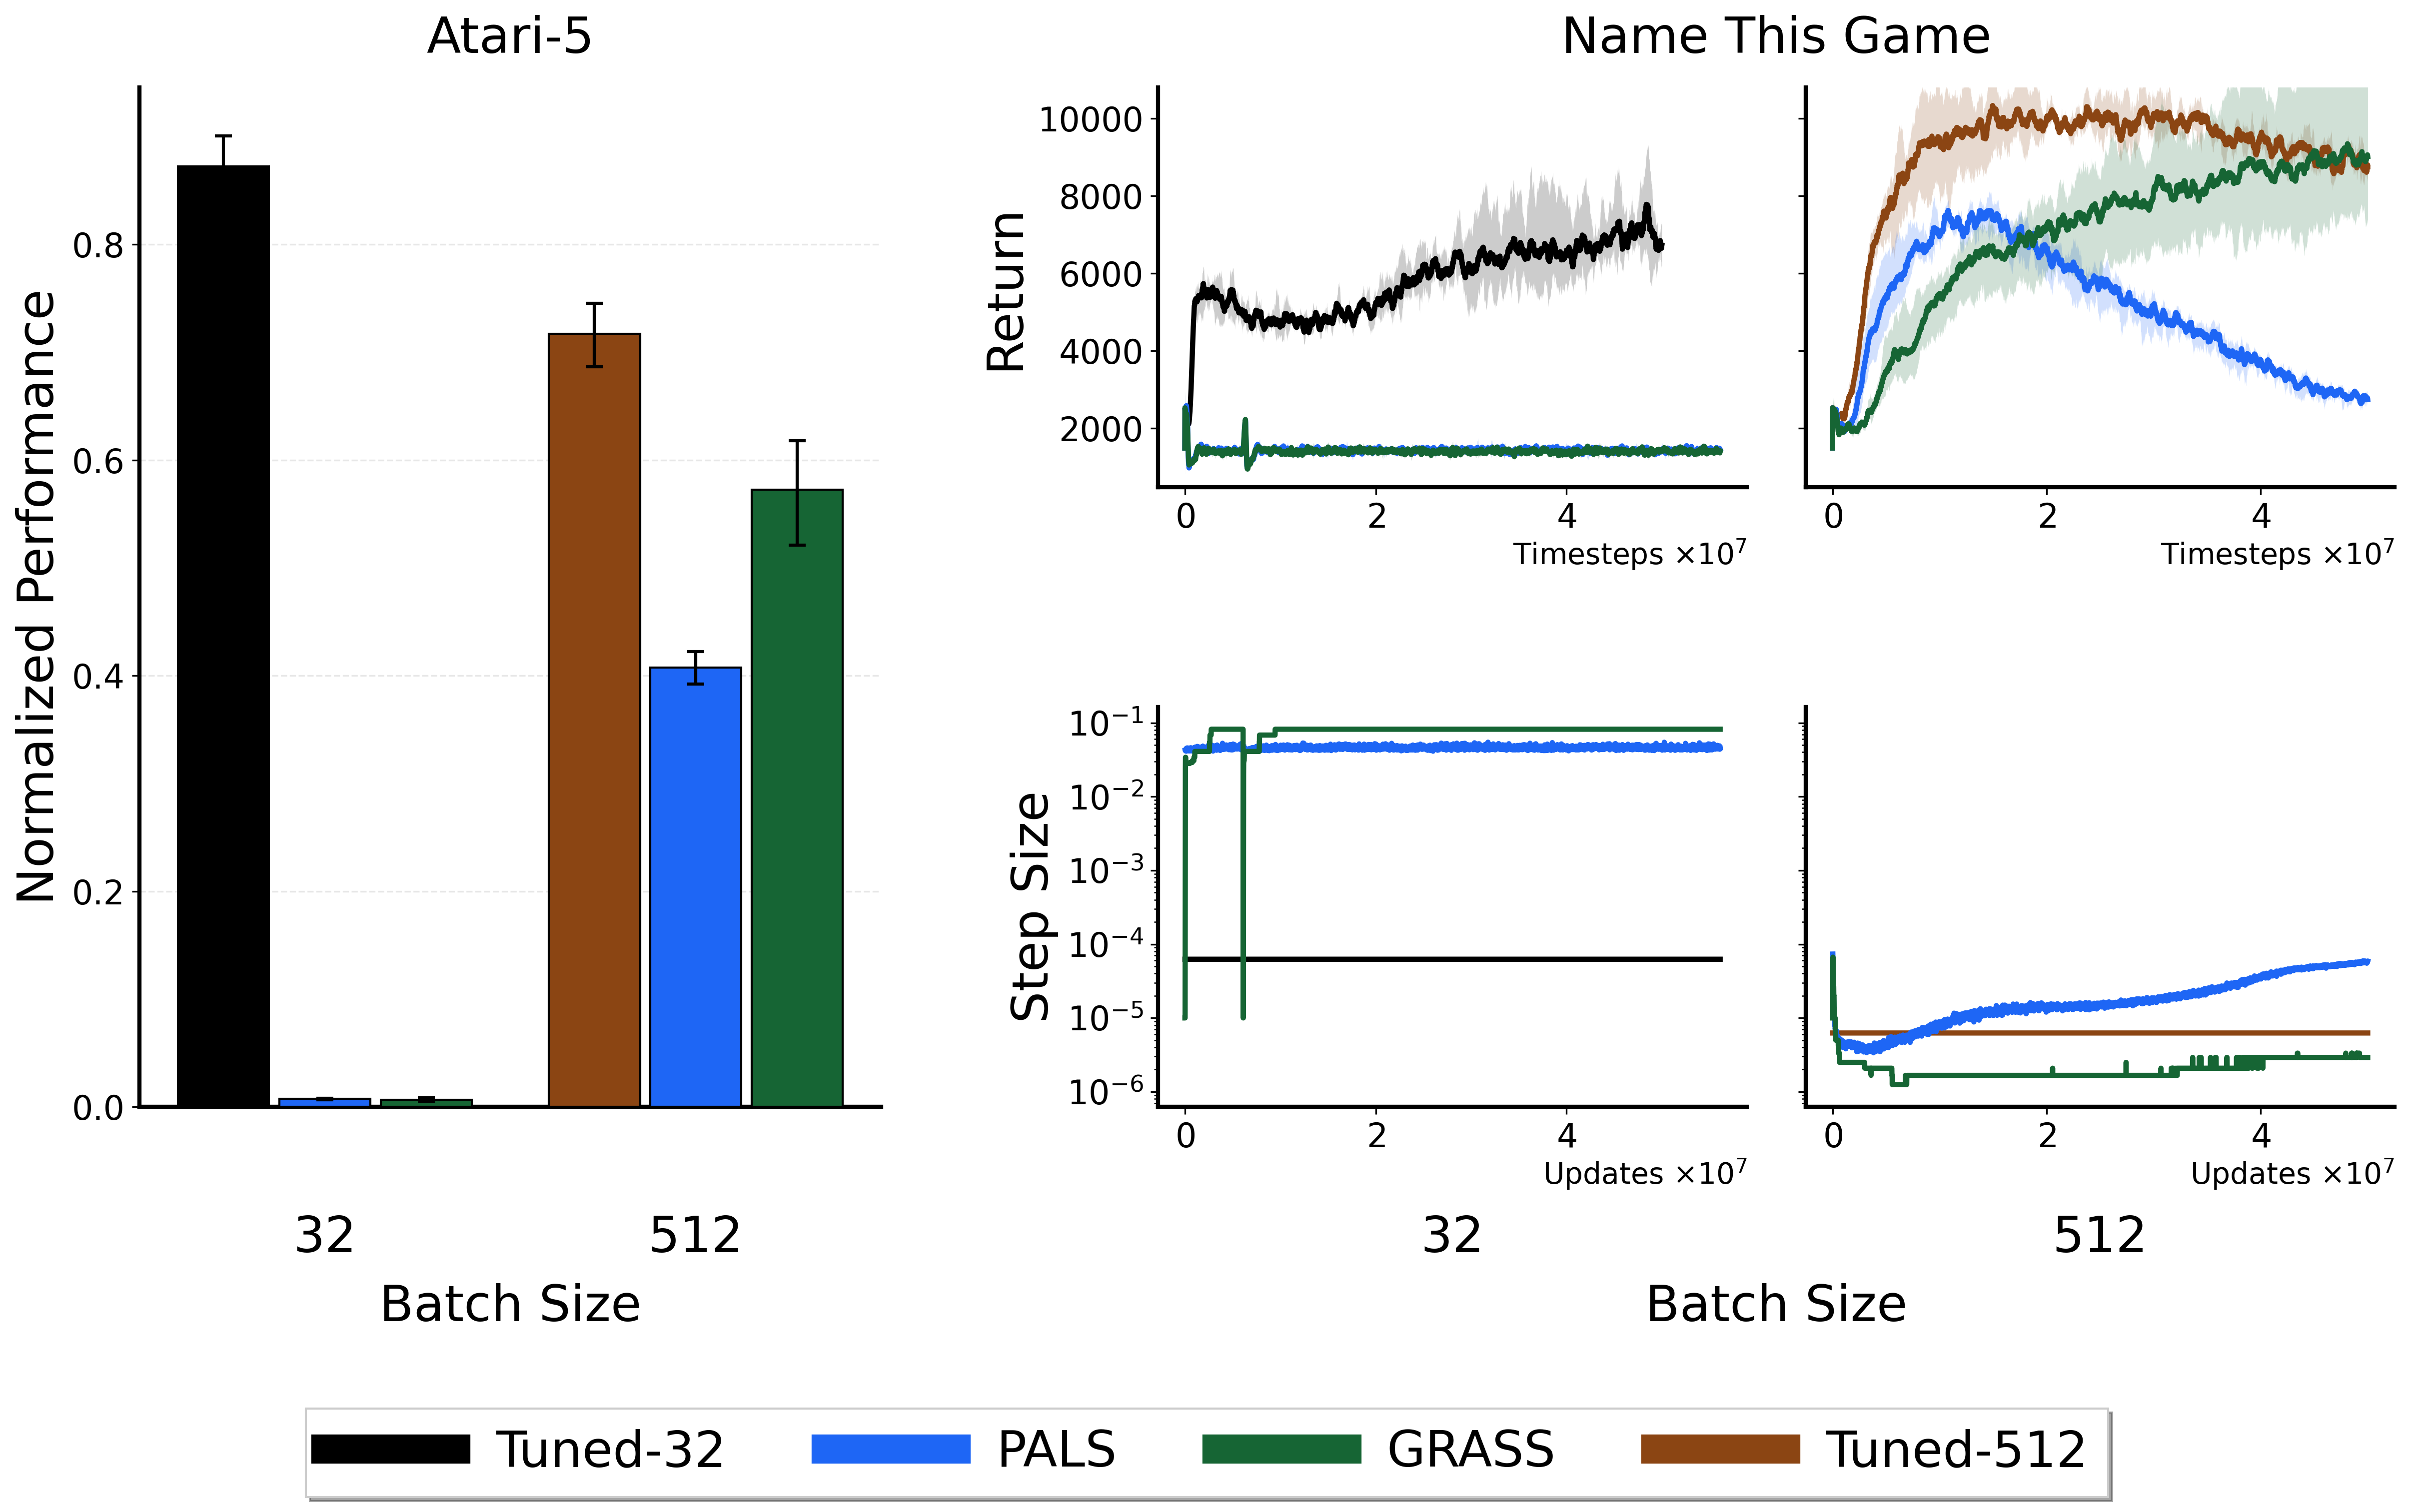
\includegraphics[width=\textwidth]{figures/thesis/ablations/2_batch_size/batch_dqn_atari5_step.png}
    \caption[Effect of batch size on DQN with Adam on Atari-5.]{Effect of batch size on DQN with Adam on Atari-5: \textbf{(a) Left:} normalized performance for GRASS and PALS with batch size 32 vs.\ 512. \textbf{(b) Right:} return and step size in Name This Game. A larger batch size massively improved performance for both methods, which completely failed to learn at batch size 32.}
    \label{fig:batch_dqn_atari}
\end{figure}

\begin{figure}[htbp]
    \centering
    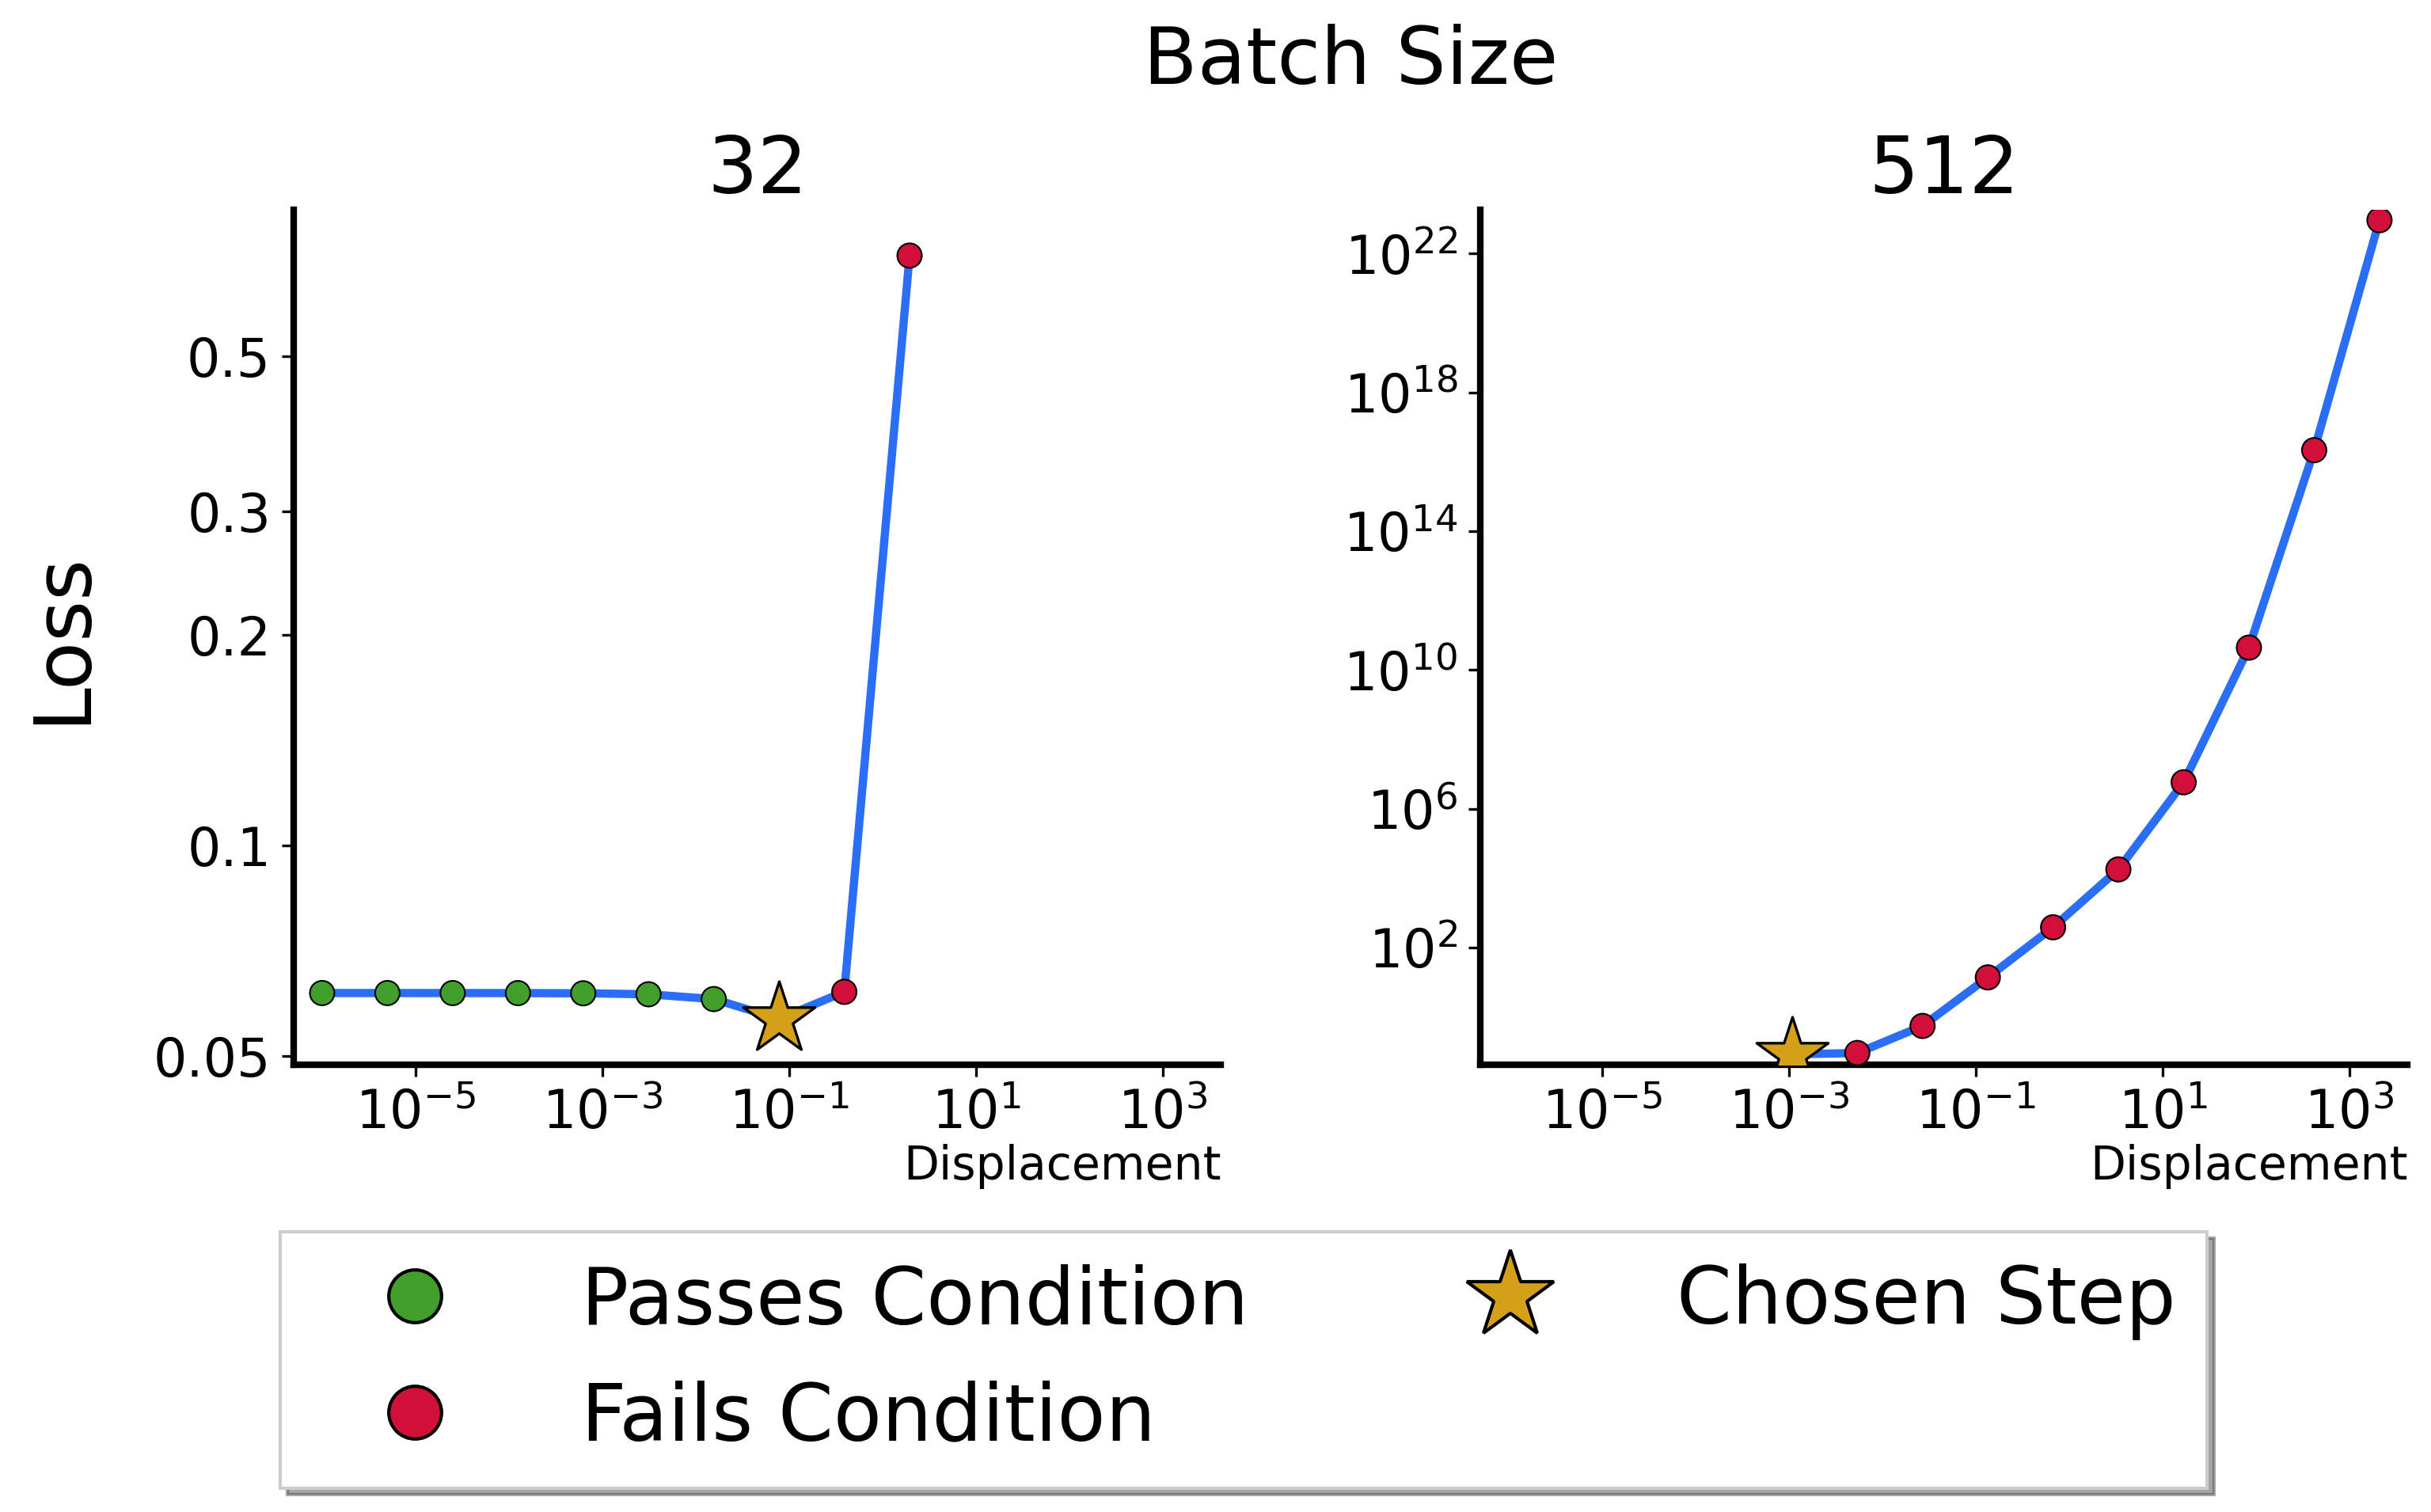
\includegraphics[width=\textwidth]{figures/thesis/ablations/2_batch_size/batch_dqn_name_this_game_stepsize_loss.png}
    \caption[Loss landscape approximation for PALS in Name This Game.]{Loss landscape approximation along the update direction for PALS in Name This Game with small and large batch size. The loss was smoother on the small batch, allowing PALS to accept a larger step size.}
    \label{fig:batch_dqn_name_this_game_loss}
\end{figure}

% PPO
Turning to PPO in Brax, we again found that all adaptive methods performed much better with large batch size, as shown in Figure~\ref{fig:batch_ppo_mujoco}(a).
Figure~\ref{fig:batch_ppo_mujoco}(b) shows actor and critic step sizes in Humanoid, where we observed that actor step sizes were much larger at batch size 64 for the line search methods (flatlining at 1, the maximum value in the search) and basic trust region. By contrast, actor step size differed by less than an order of magnitude between batch size 64 and 1024 for GRASS and the Cauchy point method. Critic step size was relatively consistent between the two batch sizes for all adaptive methods. The poor performance associated with an actor step size of 1 is unsurprising in these high-dimensional control environments. More notably, the large differences in performance for GRASS and the Cauchy point for relatively small changes in actor step size reflect the sensitivity of PPO to the actor step size in these environments.
\begin{figure}[htbp]
    \centering
    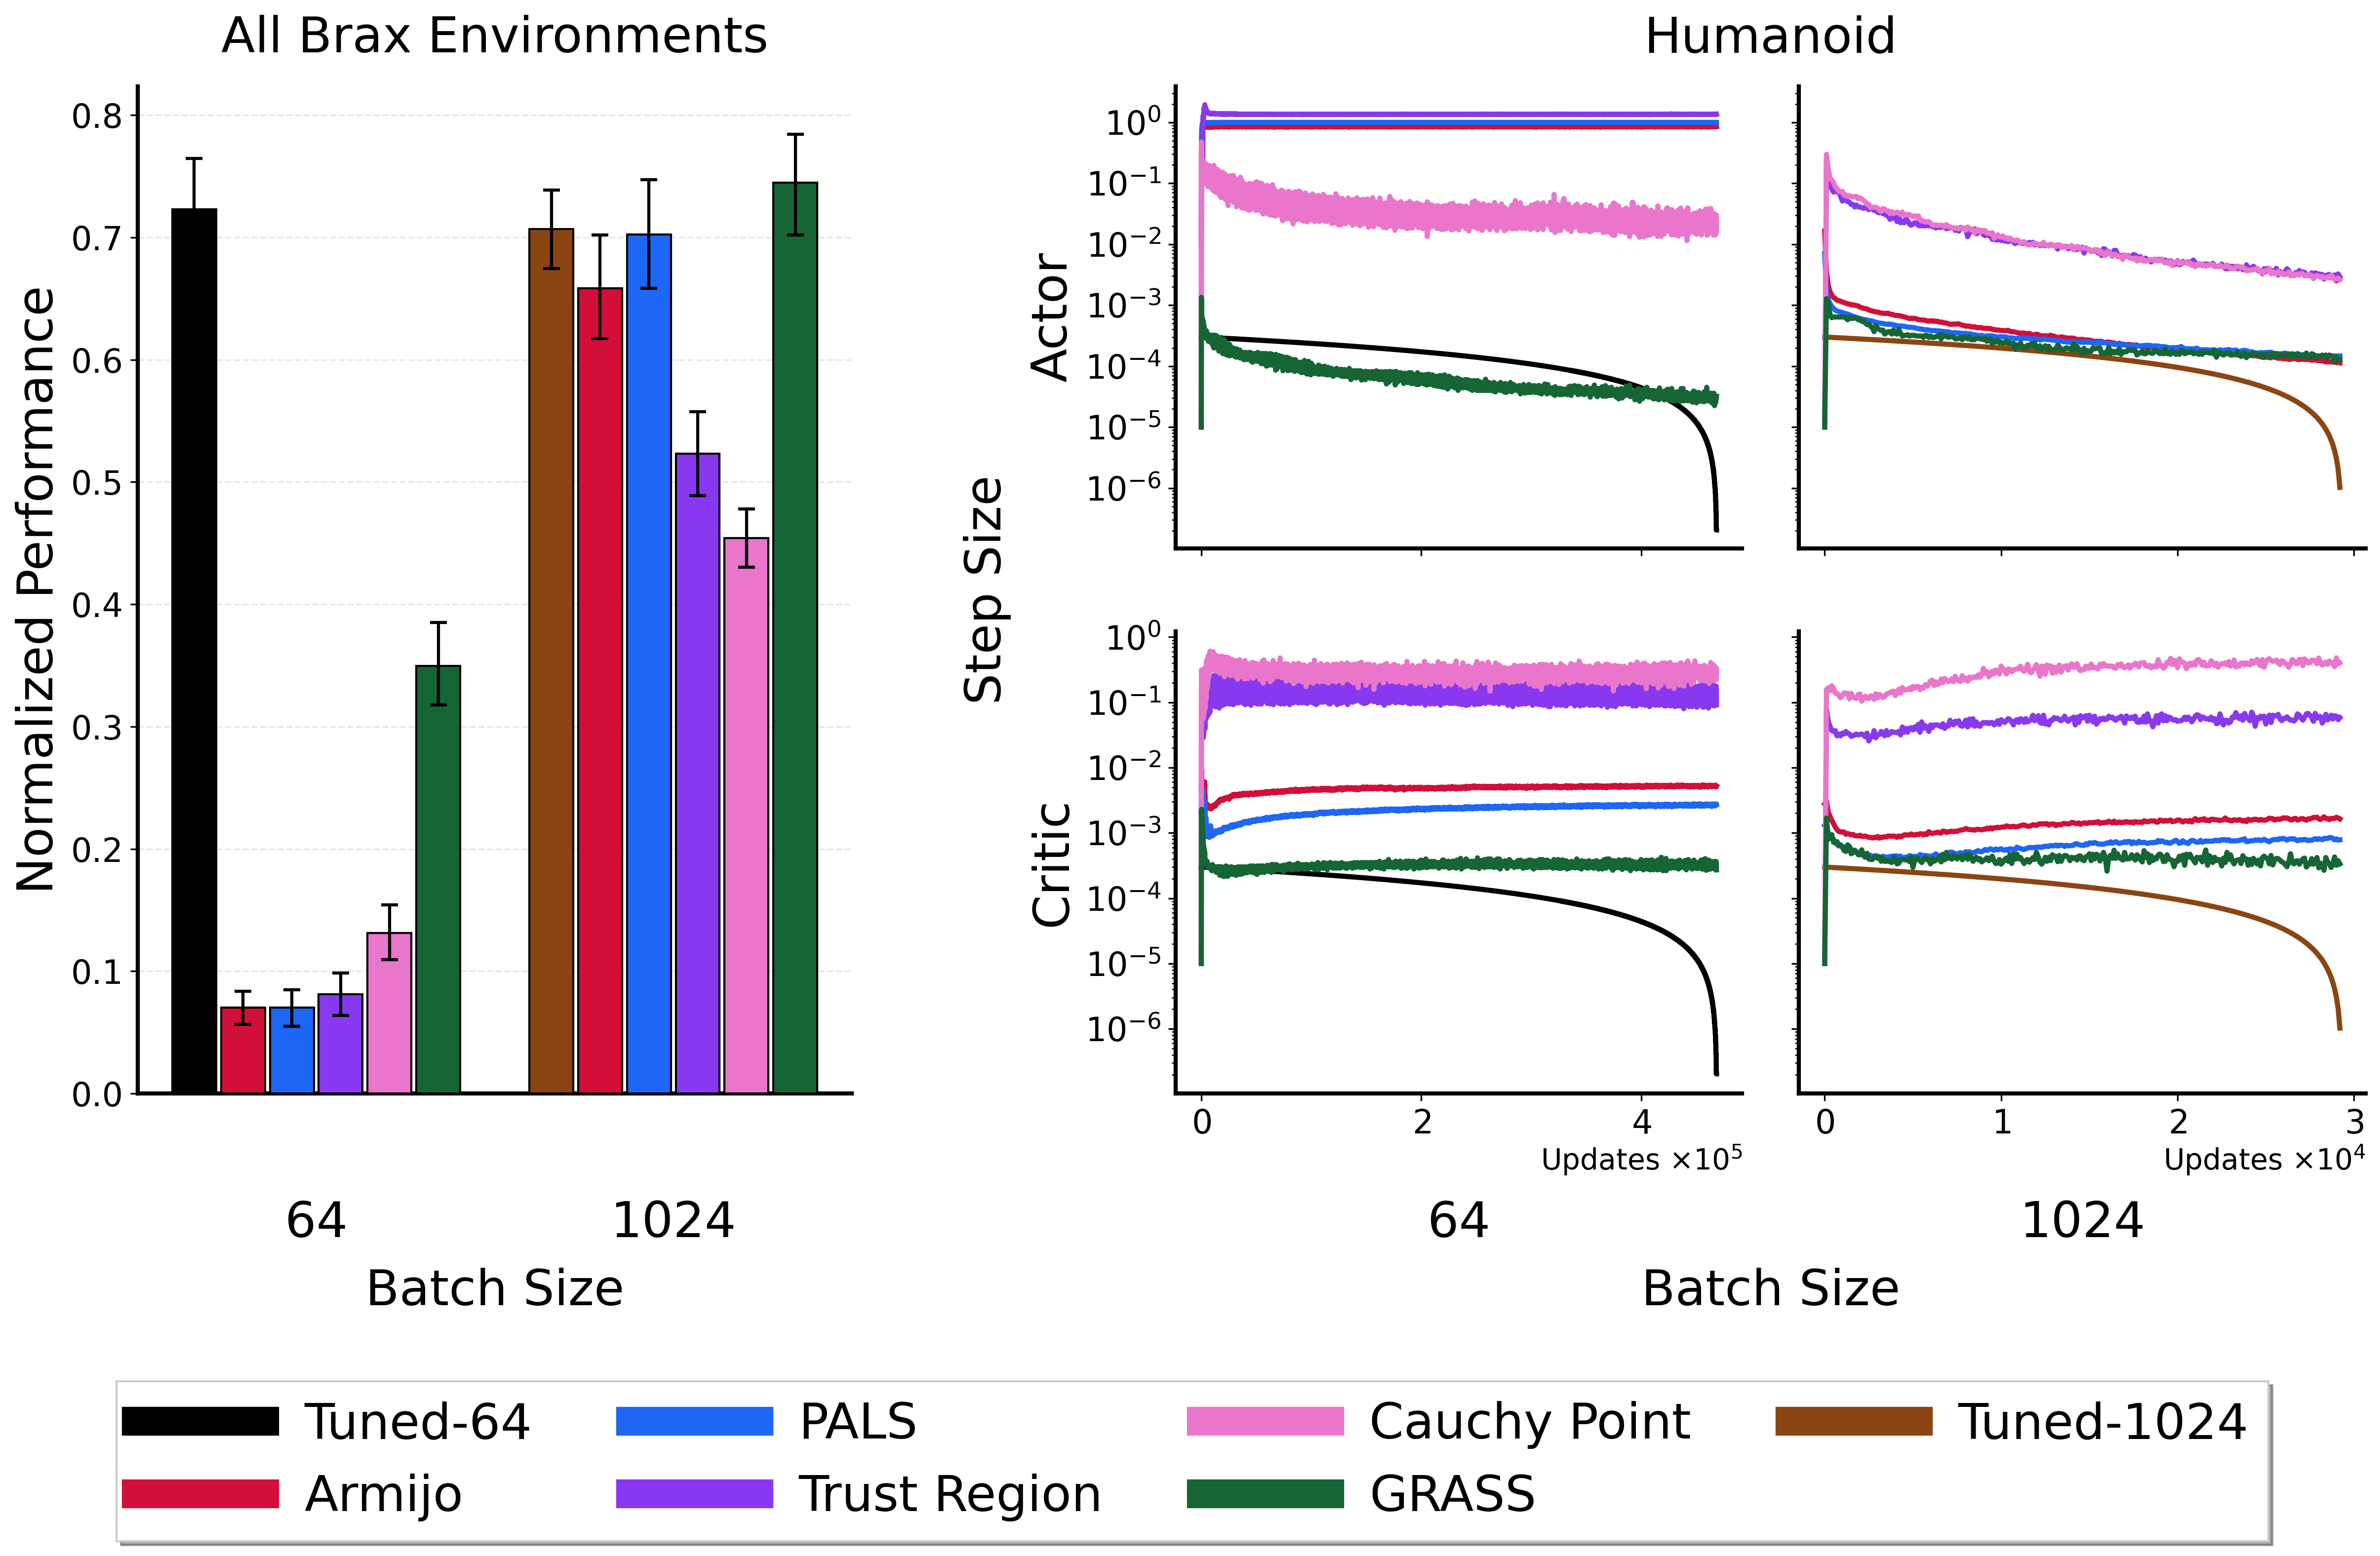
\includegraphics[width=\textwidth]{figures/thesis/ablations/2_batch_size/batch_ppo_mujoco_step.png}
    \caption[Effect of batch size on PPO with Adam in Brax.]{Effect of batch size on PPO with Adam in Brax: \textbf{(a) Left:} normalized performance for batch size 64 vs.\ 1024. \textbf{(b) Right:} Actor and critic step size in Humanoid. All adaptive methods performed much better with larger batch size.}
    \label{fig:batch_ppo_mujoco}
\end{figure}

\section{Globalization Strategies with Momentum}
We now examine the effect of removing the momentum term $m_k$
from step size selection when applying globalization strategies with Adam. When using the Adam update $u_k$ to select step size, we handle ascent directions by defaulting to the smallest candidate step size $\stepSizeInit \beta^B$ with line search and using $\rho=0.5$ for the corresponding step in the median gain-ratio with trust region methods, though we find this rarely occurs in practice. Figure~\ref{fig:adamdir_dqn_atari}(a) compares normalized performance in the Atari-5 for GRASS and PALS with and without using momentum in step size selection.
\begin{figure}[htbp]
    \centering
    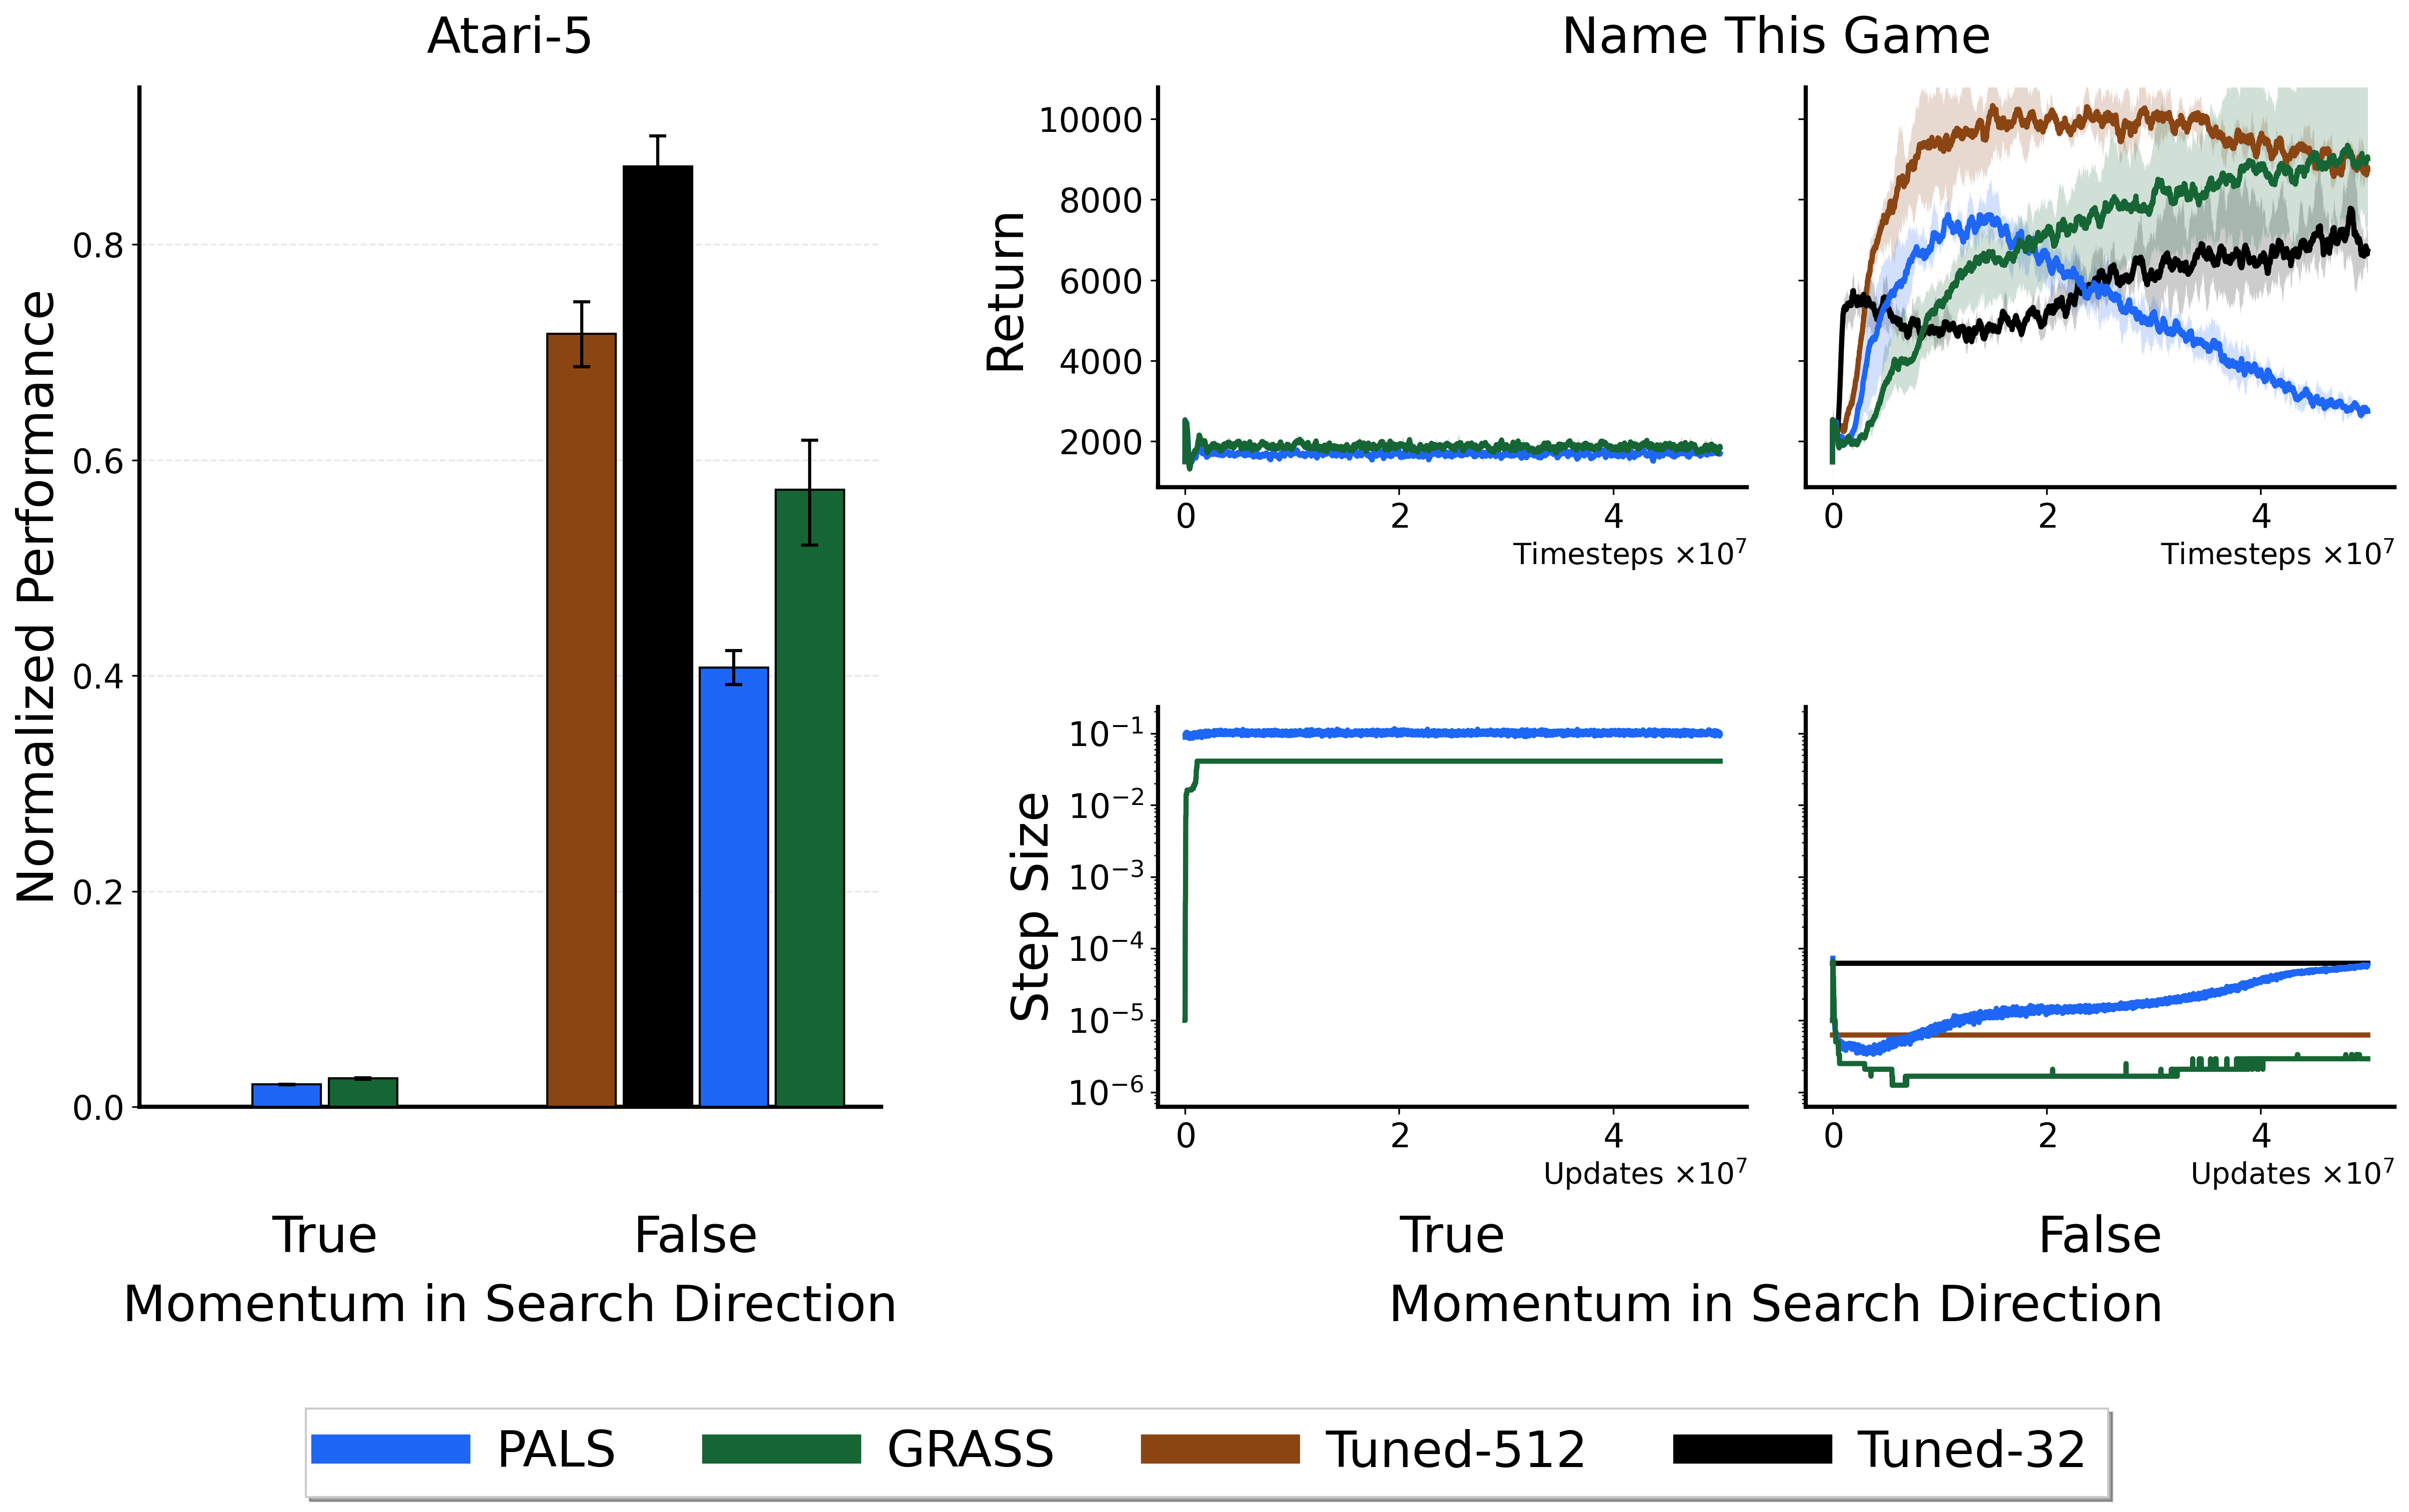
\includegraphics[width=\textwidth]{figures/thesis/ablations/3_adam_direction/adamdir_dqn_atari5_step.png}
    \caption[Ablating Momentum in Step Size Identification for DQN on Atari-5.]{Ablating the use of momentum in step size selection for DQN with Adam on the Atari-5. \textbf{(a) Left:} normalized performance across the suite and \textbf{(b) Right:} return and step size in Name This Game, with and without momentum use in step size selection. Both GRASS and PALS failed entirely when selecting step size directly with the Adam direction.}
    \label{fig:adamdir_dqn_atari}
\end{figure}
We observed that both methods failed entirely with momentum in step selection. Examining Figure~\ref{fig:adamdir_dqn_atari}(b), we found that the chosen step sizes were roughly $10^5$ times larger in Name This Game when step size selection was performed directly with $u_k$. Interestingly, this is the opposite effect of what has been observed when combining globalization strategies and momentum-based optimizers in supervised learning, where frequent ascent directions result in all step sizes being rejected \tocite{paper that does ls with amsgrad}.

Investigating further, Figure~\ref{fig:adamdir_dqn_name_this_game_loss} shows an approximation of the loss landscape in Name This Game for a typical update when using both the momentum and no-momentum selection strategies with PALS. Similar to the finding for small batch size, when using $u_k$ in the search, the actual loss matched the first-order model over a much larger distance in parameter space than for $\hat{u}_k$, allowing for a larger accepted step size. When removing momentum from the search direction, the curvature was sharper, resulting in more conservative steps. \todo{Q for Adam: have spent too much time trying to figure so tabling for now, but still not clear to me why this is the case, any thoughts?}

\begin{figure}[htbp]
    \centering
    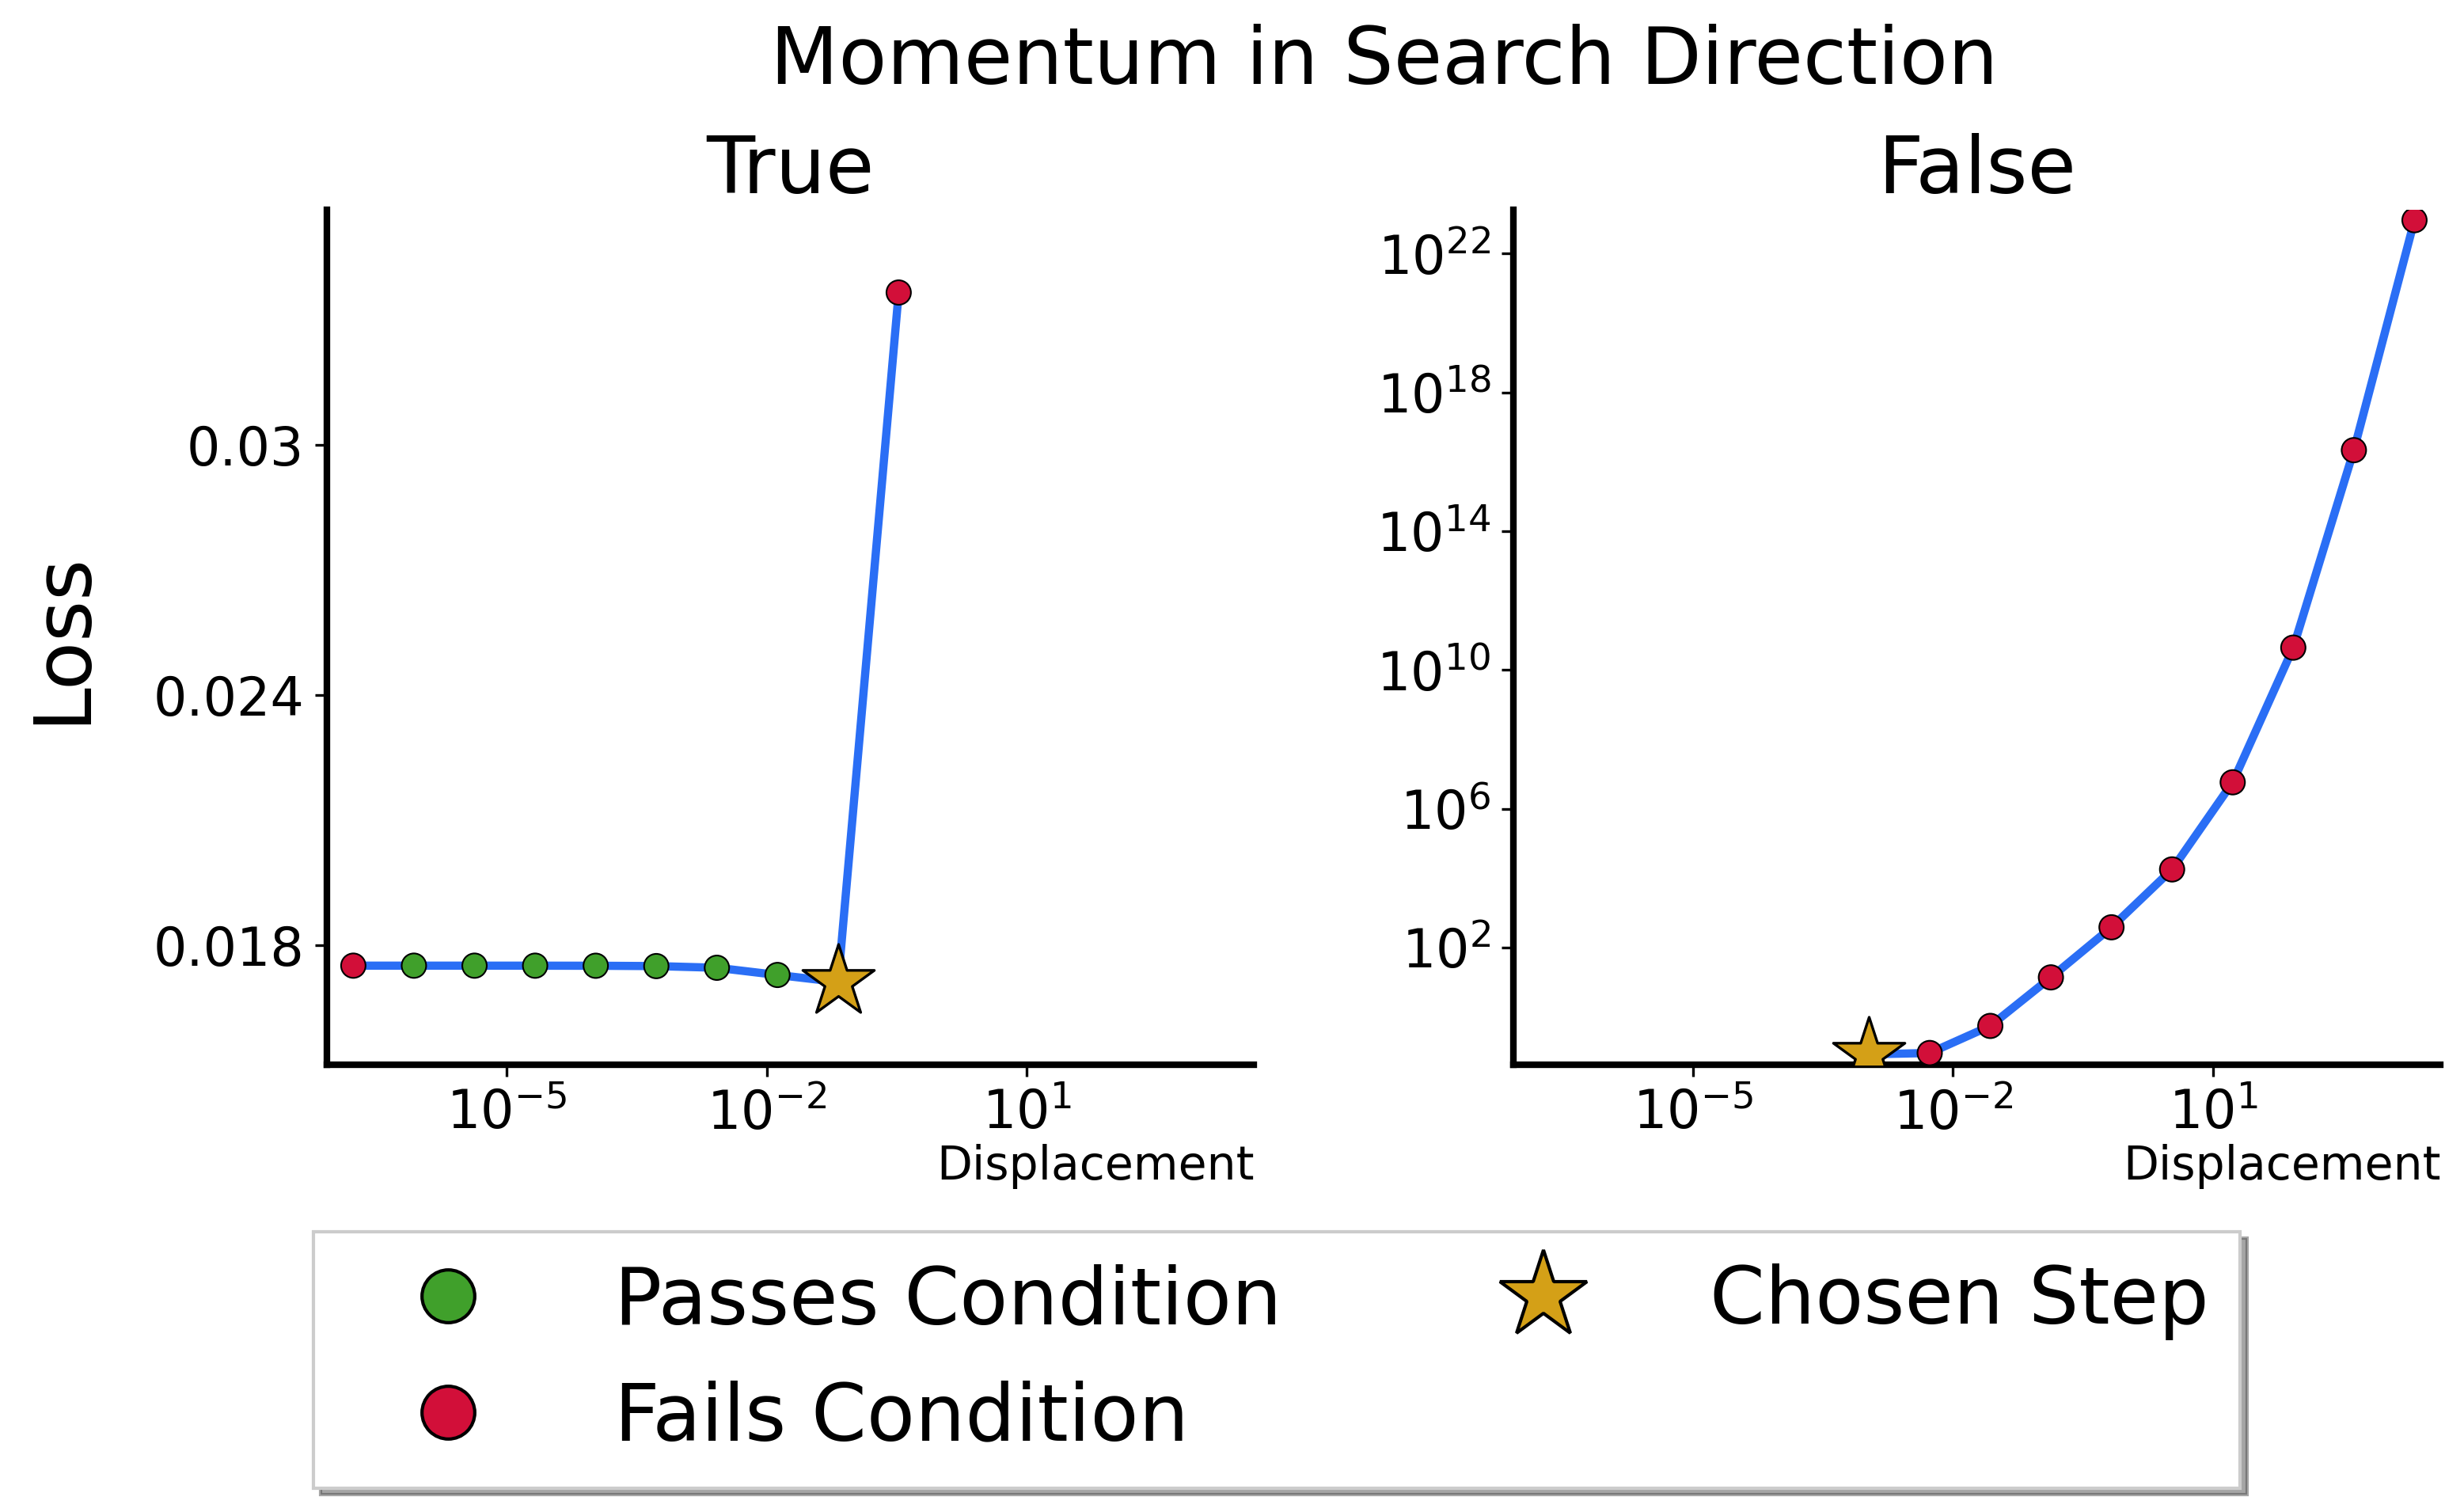
\includegraphics[width=\textwidth]{figures/thesis/ablations/3_adam_direction/adamdir_dqn_name_this_game_stepsize_loss.png}
    \caption[Loss landscape approximation for the momentum ablation in Name This Game.]{Loss landscape approximation along the update direction for PALS in Name This Game, with and without momentum in step size selection. The loss matched the first-order model over a much larger distance when using the momentum direction $u_k$, allowing for a larger accepted step size.}
    \label{fig:adamdir_dqn_name_this_game_loss}
\end{figure}

Turning to PPO in Brax, we observed that performance was also greatly improved for all methods when using $\hat{u}_k$ in place of $u_k$ when selecting step size, as shown in Figure~\ref{fig:adamdir_ppo_mujoco}(a).
\begin{figure}[htbp]
    \centering
    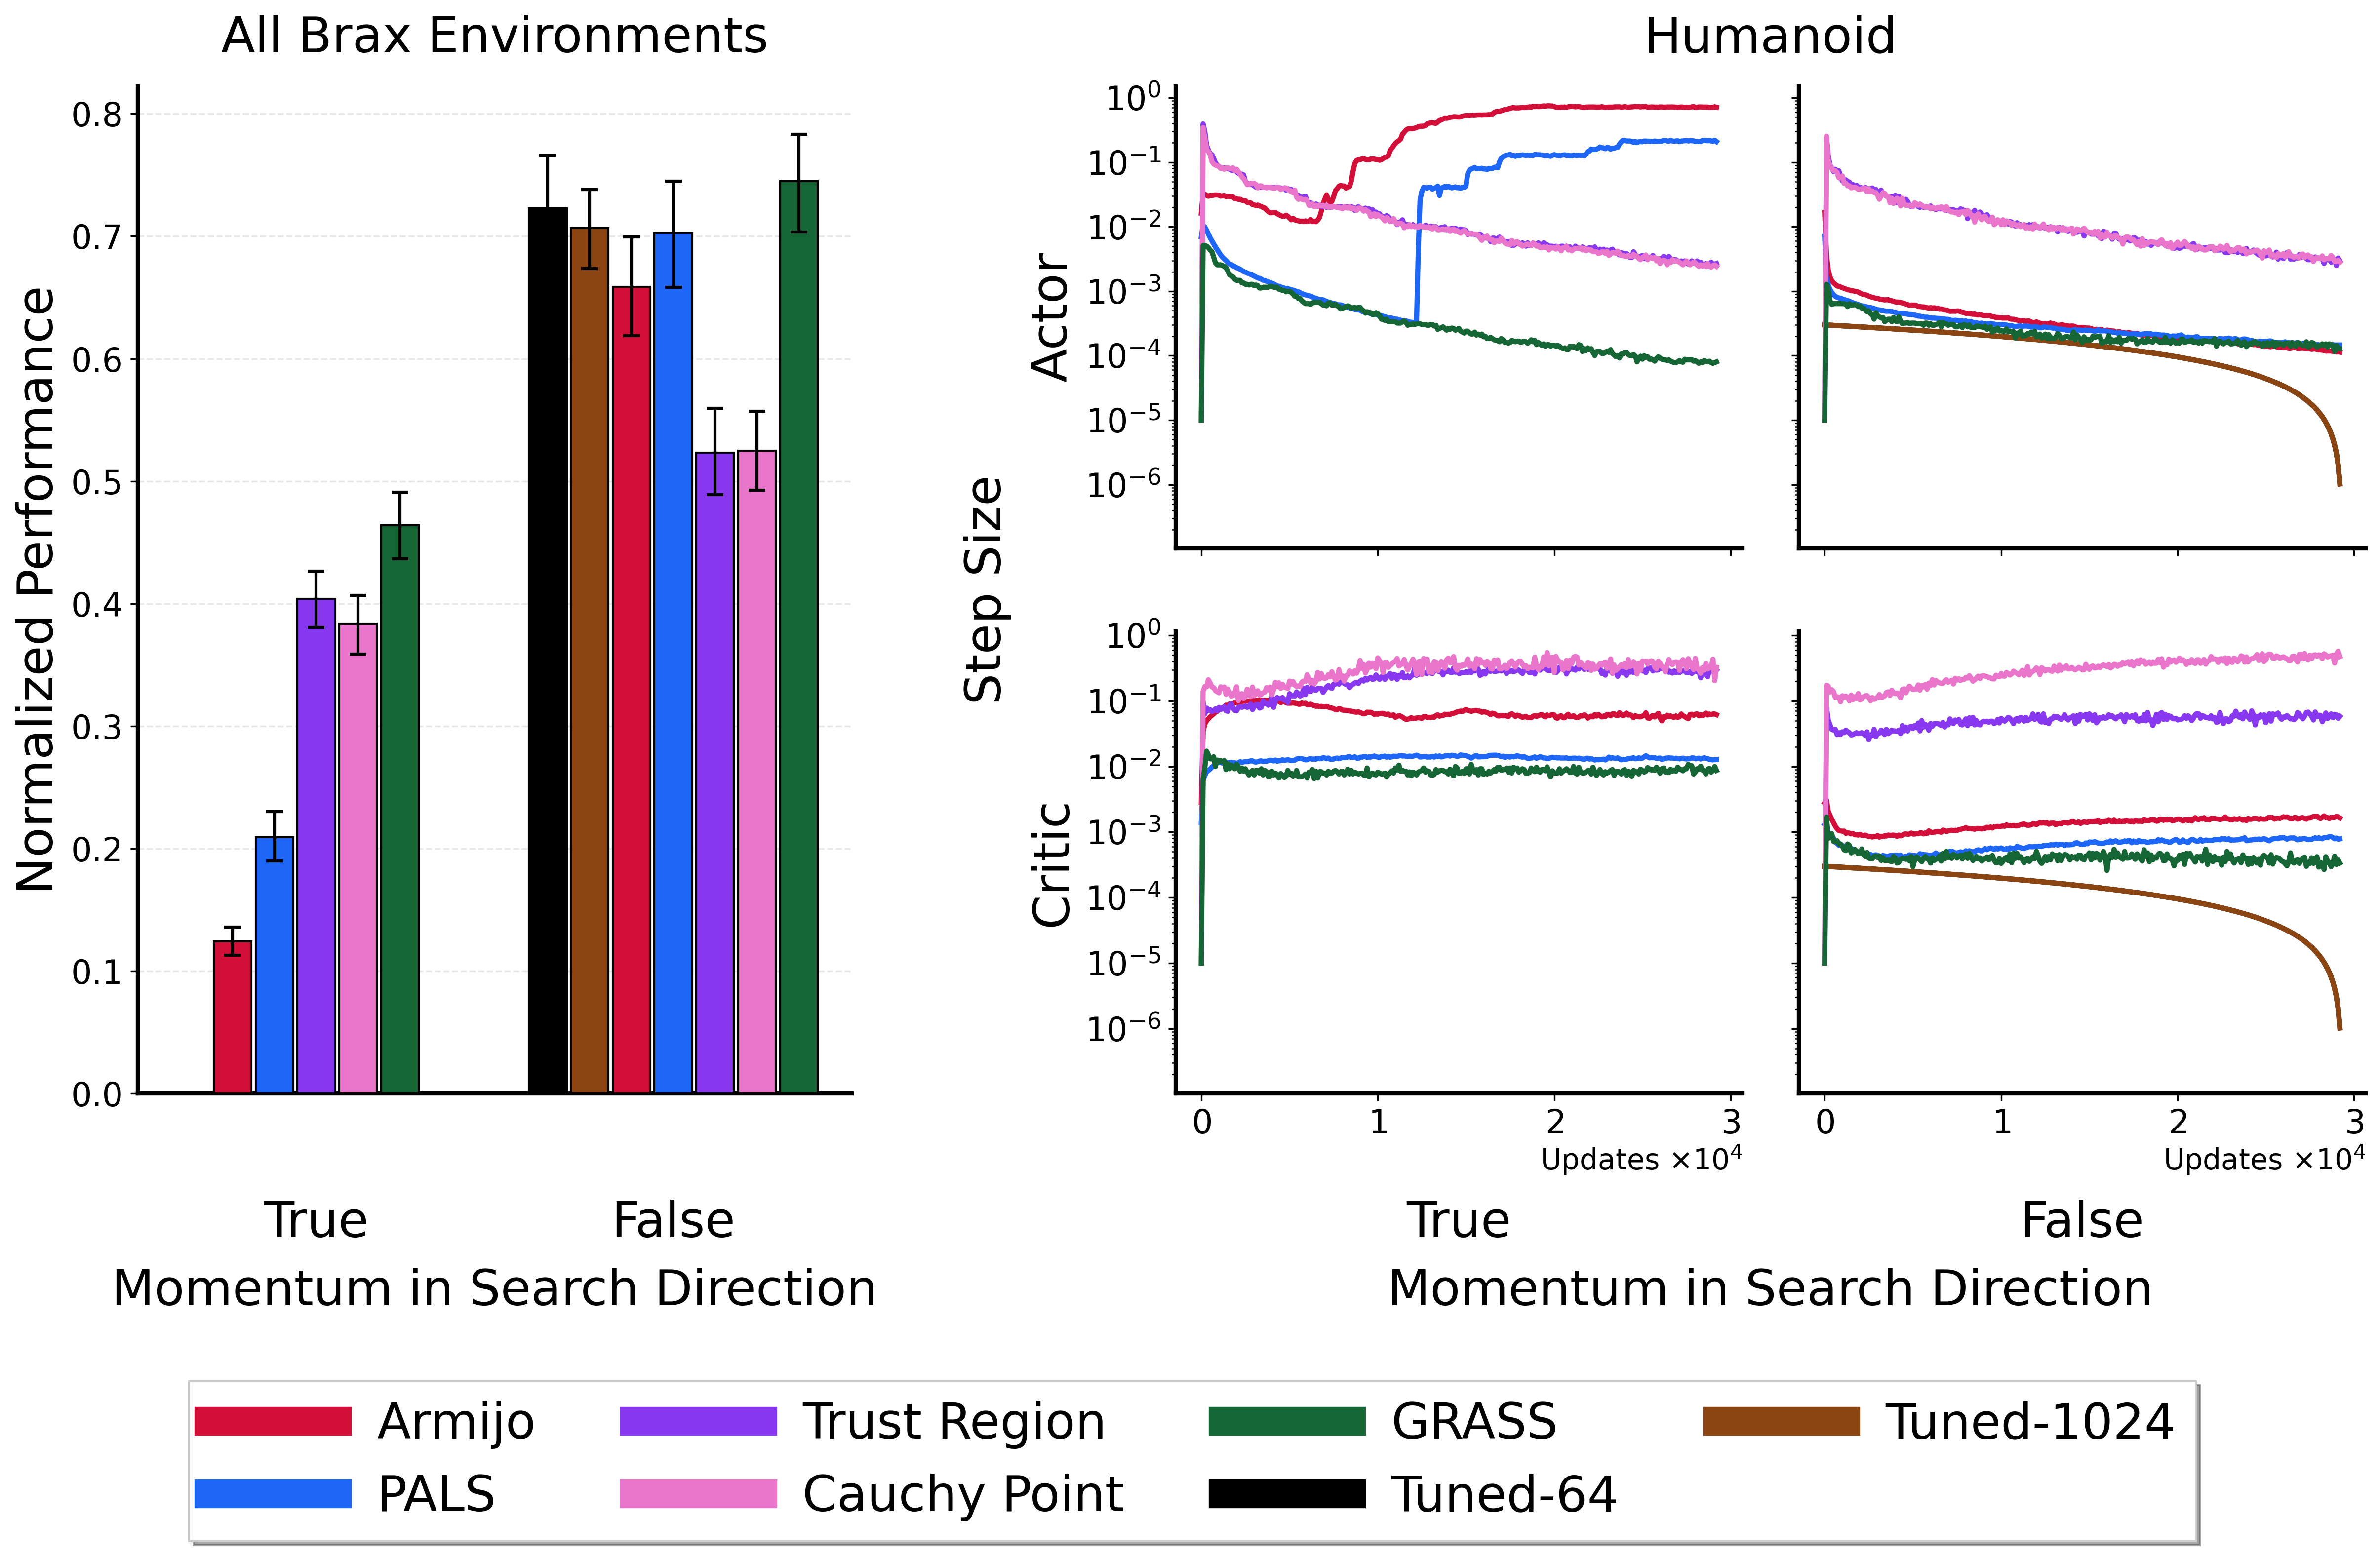
\includegraphics[width=\textwidth]{figures/thesis/ablations/3_adam_direction/adamdir_ppo_mujoco_step.png}
    \caption[Ablating Momentum in Step Size Identification for PPO in Brax.]{Ablating Momentum in Step Size Identification for PPO with Adam in Brax: \textbf{(a) Left:} normalized performance across the suite and \textbf{(b) Right:} actor/critic step size in Humanoid, with and without momentum in step size selection. Performance was greatly improved for all methods when excluding momentum from step size selection.}
    \label{fig:adamdir_ppo_mujoco}
\end{figure}
In Figure~\ref{fig:adamdir_ppo_mujoco}(b), we found that the actor step sizes for the line search were much larger than the tuned baseline when using $u_k$, while they were within an order of magnitude with $\hat{u}_k$. For GRASS and the trust region methods, the actor step sizes were consistent between the two variants, but the critic step size was larger when using momentum in selection. Figure~\ref{fig:adamdir_ppo_humanoid_loss} shows approximations of the actor and critic losses for PALS in Humanoid. Similarly to DQN, we observed that the larger critic step sizes were a product of smoother loss along the momentum direction, though the actor was less afftected. \todo{add comment about why this is, but still not sure as above with DQN}.

\begin{figure}[htbp]
    \centering
    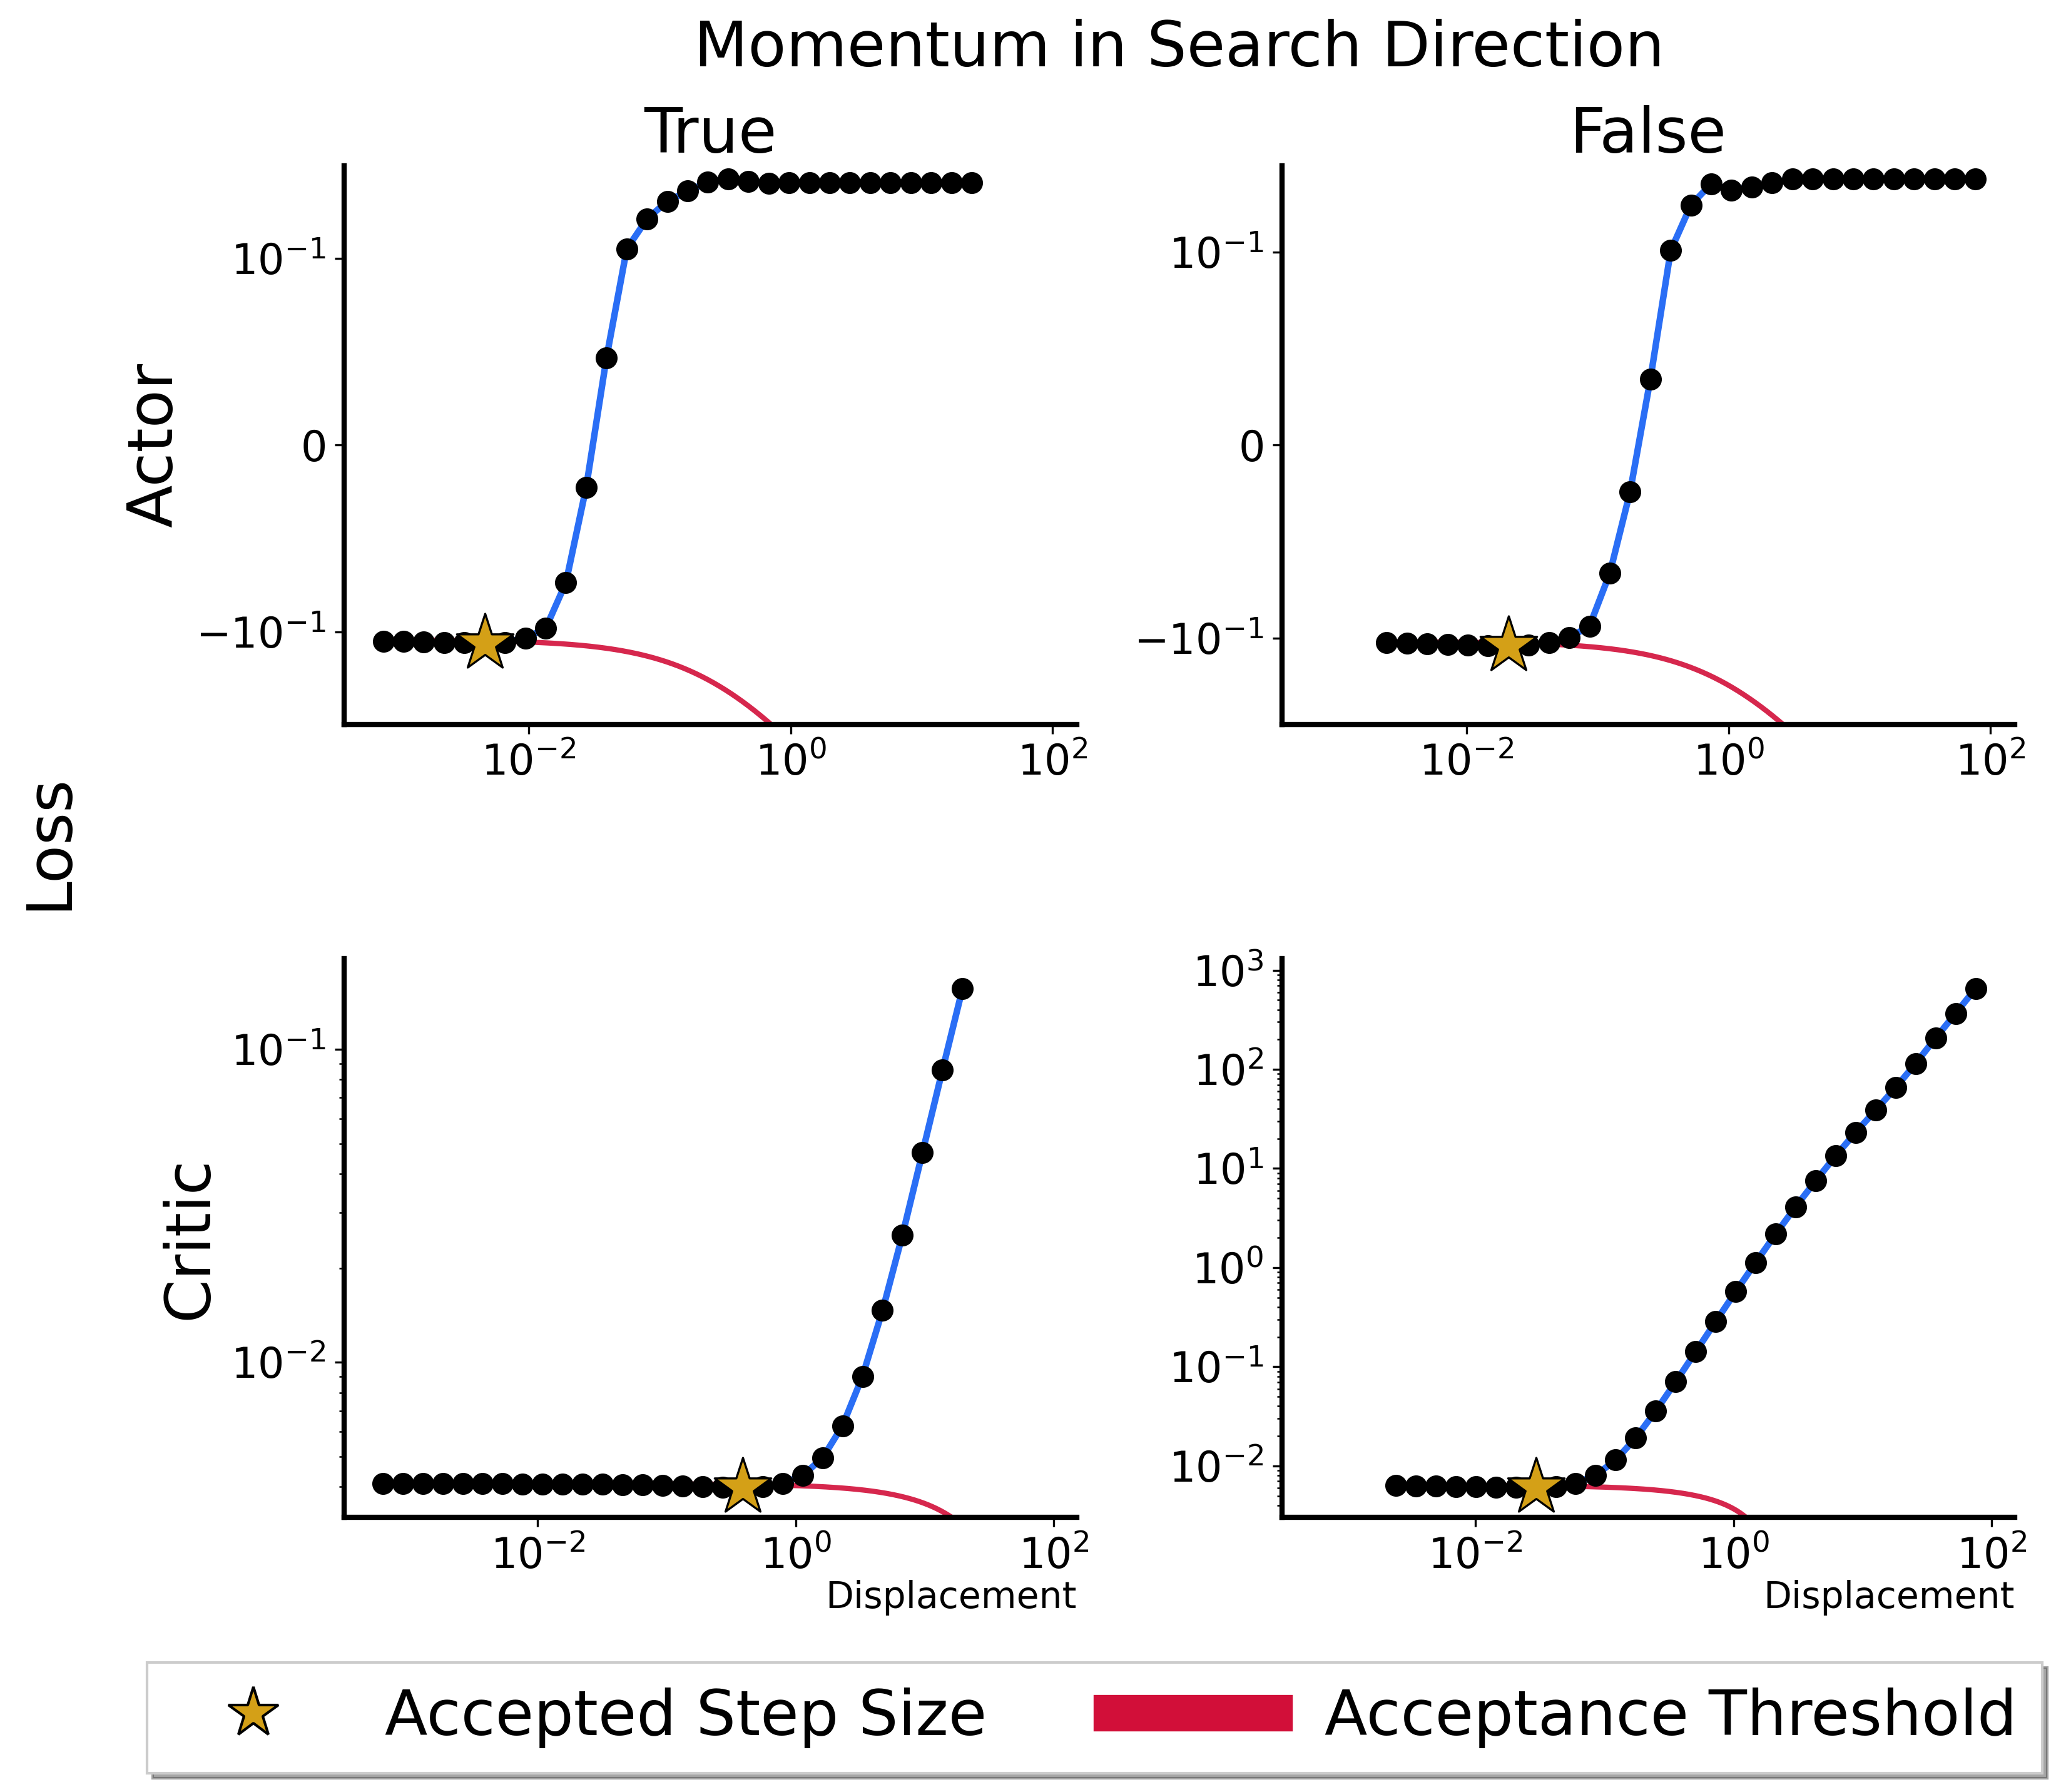
\includegraphics[width=0.72\textwidth]{figures/thesis/ablations/3_adam_direction/adamdir_ppo_humanoid_stepsize_loss.png}
    \caption[Loss landscape approximation for the momentum ablation in Humanoid.]{Approximations of the actor and critic loss along the update direction for PALS in Humanoid, with and without momentum in step size selection. The larger critic step sizes with momentum were a product of smoother loss along the momentum direction, though the actor loss appeared unaffected.}
    \label{fig:adamdir_ppo_humanoid_loss}
\end{figure}

\section{Comparing the Median and Single-Step Gain-Ratio} \label{sec:gain_ratio_ablation}
We compare the traditional single-step gain-ratio (Equation~\eqref{eq:tr_ratio}) against the median gain-ratio over a window of $K$ updates introduced in GRASS (Algorithm~\ref{alg:grass}), which we applied with all trust-region-based methods in all experiments thus far. Figure~\ref{fig:gain_ratio_window_dqn_atari}(a) examines the performance of these two approaches across the Atari-5 for GRASS.
\begin{figure}[htbp]
    \centering
    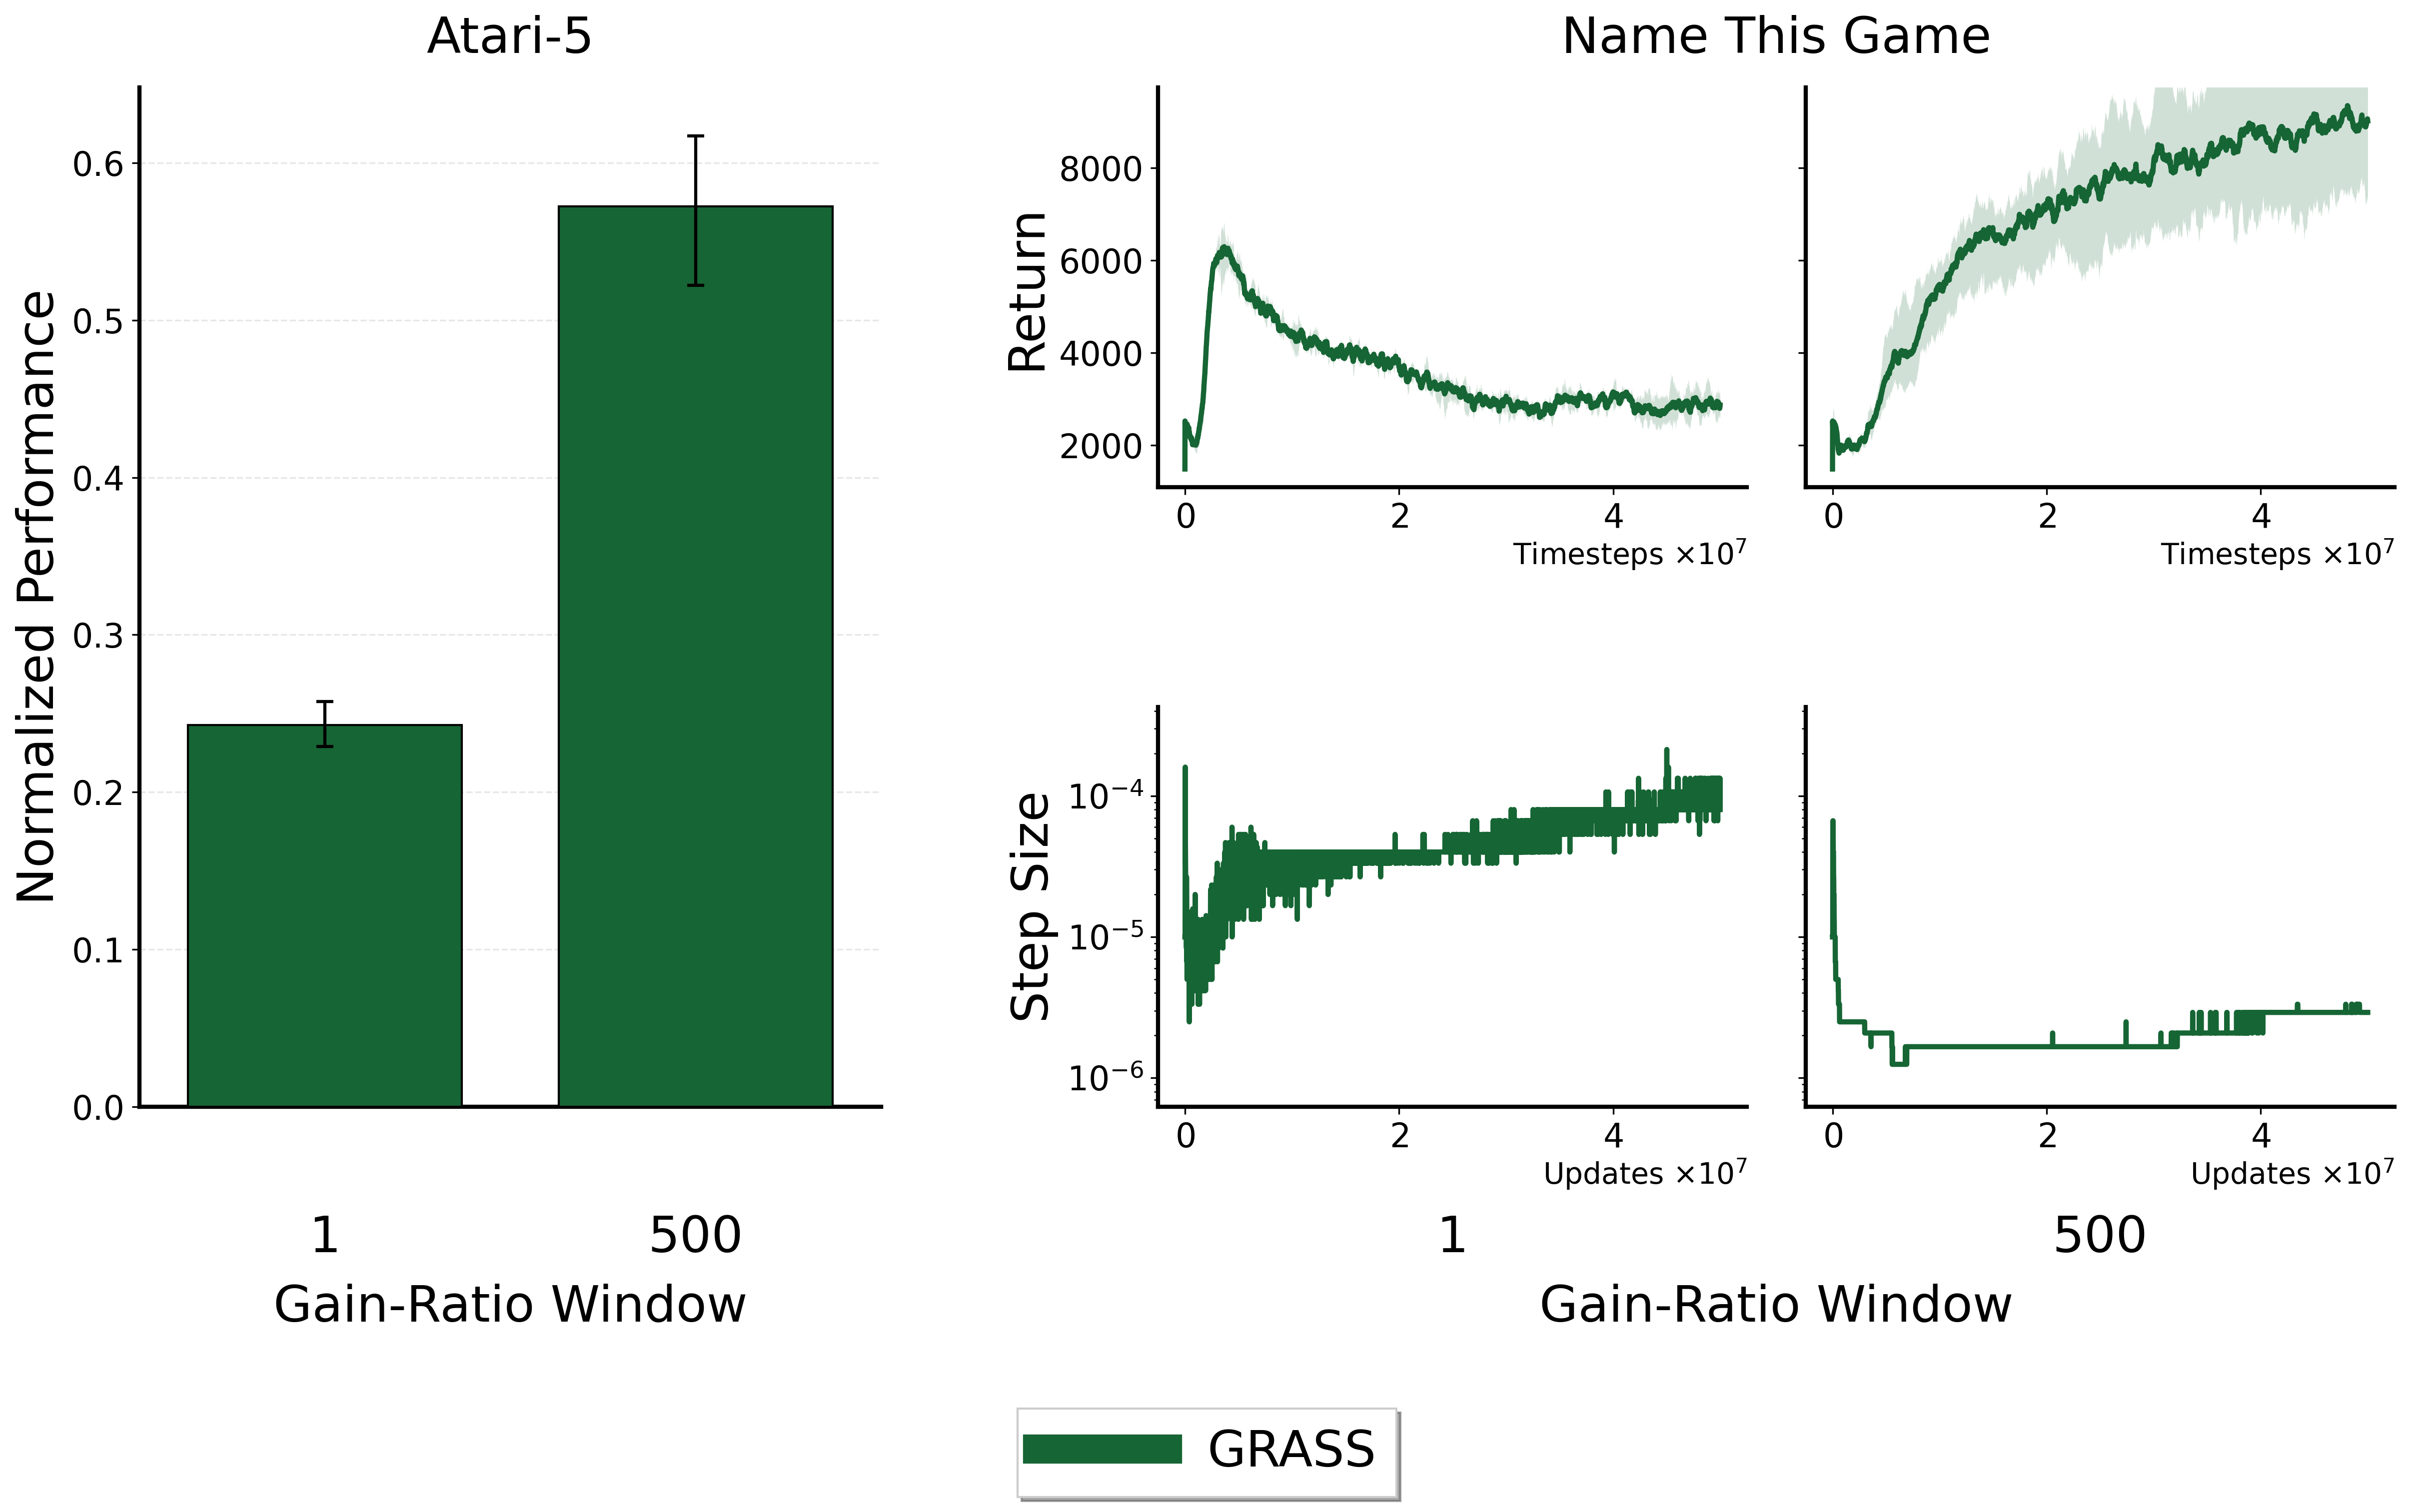
\includegraphics[width=\textwidth]{figures/thesis/ablations/4_gain_ratio_window/gain_ratio_window_dqn_atari_step.png}
    \caption[Effect of gain-ratio window on DQN with Adam on Atari-5.]{Effect of gain-ratio window on DQN with Adam on Atari-5: \textbf{(a) Left:} normalized performance for GRASS with the single-step vs.\ median gain-ratio across the suite. \textbf{(b) Right:} Return and step size in Name This Game. Performance was much improved using the median gain-ratio with window $K=500$.}
    \label{fig:gain_ratio_window_dqn_atari}
\end{figure}
\todo{note for Adam: didn't run other methods to save compute, seems like bad practice so maybe run regular TR too? note i run them all for PPO mujoco bc its cheaper} Note that a gain-ratio window of $1$ corresponds to updating the step size after every update using the single-step ratio, while the larger window matches the $K$ used in the main experiments. We observed that performance was much improved with $K$ set to 500, which corresponds to $1/4$ of the target network update interval, suggesting improved robustness to noisy gradient estimates in determining the true accuracy of the first-order model. Examining the step sizes for Name This Game in Figure~\ref{fig:gain_ratio_window_dqn_atari}(b), we found that the single-step ratio resulted in a larger accepted step size and worse performance, similar to the effect of small batch size.

Interestingly, this effect did not hold for PPO in Brax, where trust-region-based methods appeared compatible with the single-step gain ratio. Figure~\ref{fig:gain_ratio_window_ppo_mujoco}(a) shows that performance in Brax was relatively unchanged when using the single-step ratio vs.\ a ratio of $5$, which corresponds to $1/4$ of the updates per data collection phase when using batch size 1024, though GRASS was slightly improved.
\begin{figure}[htbp]
    \centering
    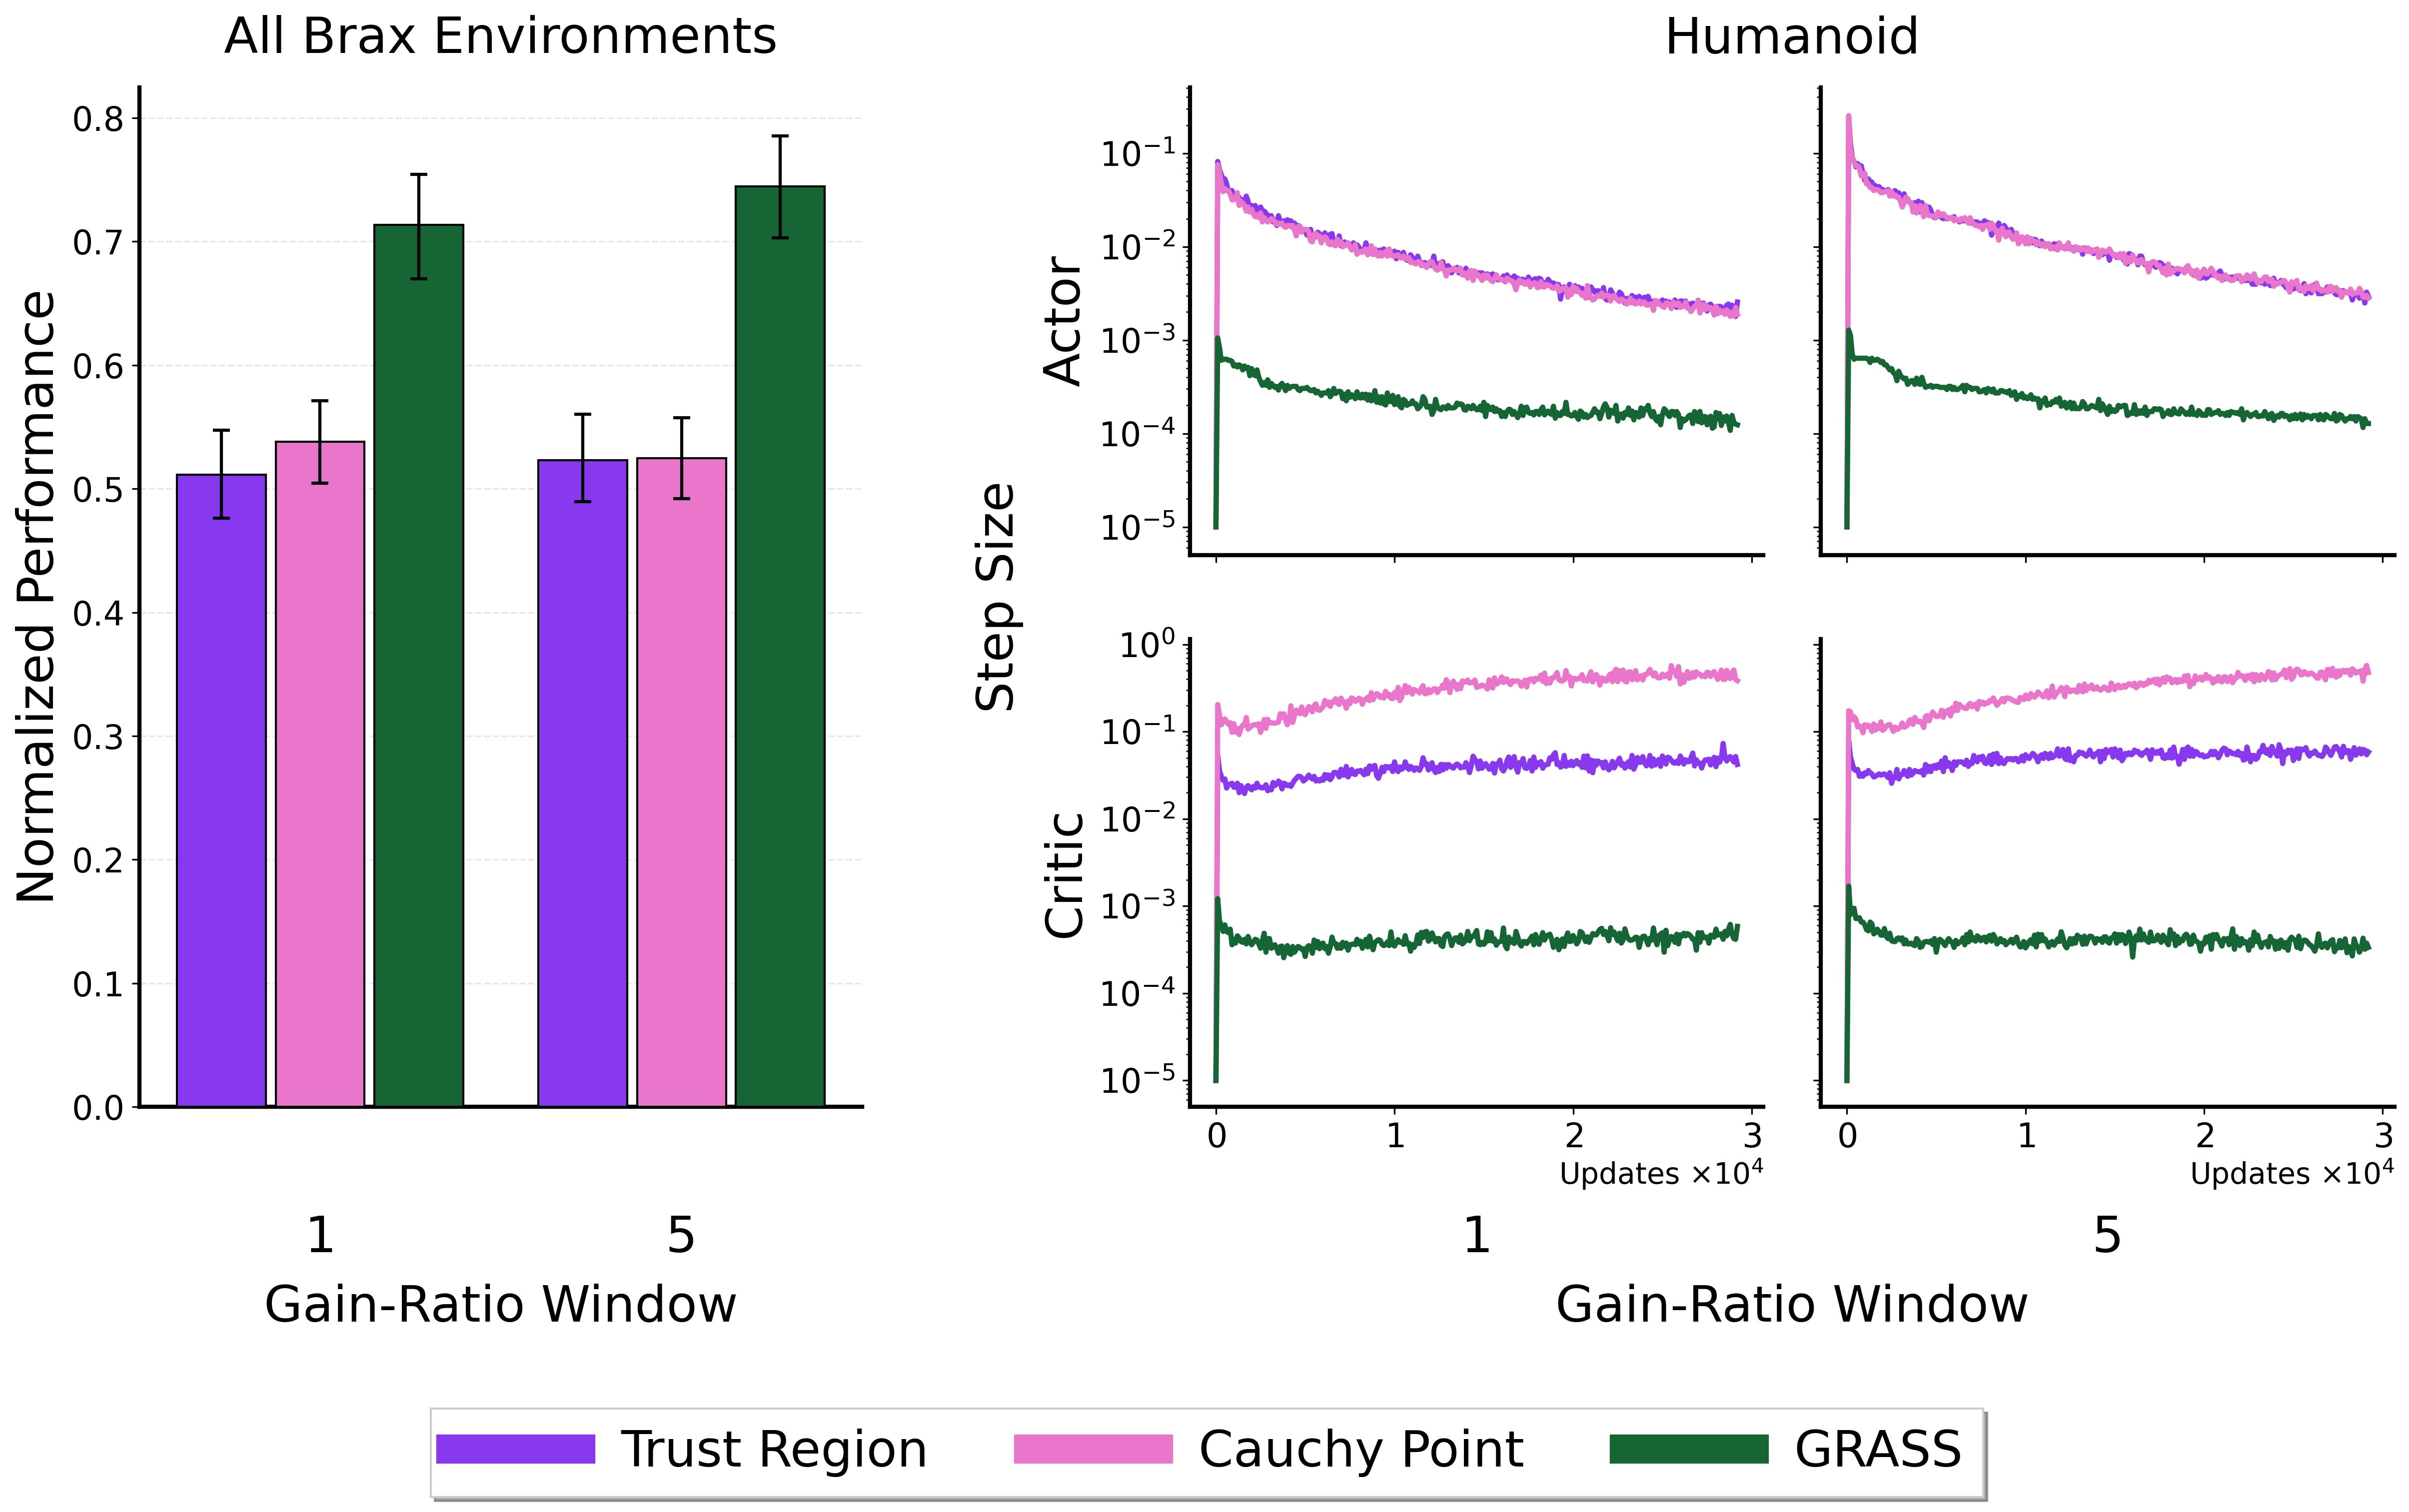
\includegraphics[width=\textwidth]{figures/thesis/ablations/4_gain_ratio_window/gain_ratio_window_ppo_mujoco_step.png}
    \caption[Effect of gain-ratio window on PPO with Adam on Brax.]{Effect of gain-ratio window on PPO with Adam on Brax. \textbf{(a) Left:} Normalized performance across the suite and \textbf{(b) Right:} step size in Humanoid, using the single-step vs.\ median gain-ratio. Performance was relatively unchanged between the two gain-ratios, though GRASS was slightly improved with the median gain-ratio.}
    \label{fig:gain_ratio_window_ppo_mujoco}
\end{figure}

We also observed that step sizes remained largely unaffected by this change, as demonstrated for Humanoid in Figure~\ref{fig:gain_ratio_window_ppo_mujoco}(b).
The lesser importance of the aggregated gain ratio with PPO is likely because the individual stochastic gradients are already serviceably low-variance. With PPO, a minibatch of $1024$ is drawn from a frozen, approximately on-policy dataset of $2048$ samples, so each $f_k$ contains half of the dataset used in the true objective, and successive batches may be very similar. This is closer to the deterministic setting for which the single-step gain-ratio was designed. With DQN, a batch of $512$ is drawn from a replay buffer of $1{,}000{,}000$ transitions collected under many past policies, so $f_k$ is derived from a relatively smaller and more diverse sample, with the resulting $\rho_k$ likely having higher variance. The decreased impact between the two treatments for PPO is also likely influenced by the much smaller difference in $K$ as compared to DQN. Importantly, this finding demonstrates the advantage of GRASS over the standard Trust Region and Cauchy Point methods is not a product of the median gain-ratio, but rather tied to using the unnormalized update vector. 

\section{Mitigating Sharp Minima with SAM}
We now return to the finding in Section~\ref{sec:dqn_results}
that globalization strategies can select overly conservative step sizes in some environments with DQN, moving into sharp regions of parameter space. We introduce a strategy for resolving this issue using Sharpness Aware Minimization as described in Section~\ref{sec:sam}.
\begin{figure}[htbp]
    \centering
    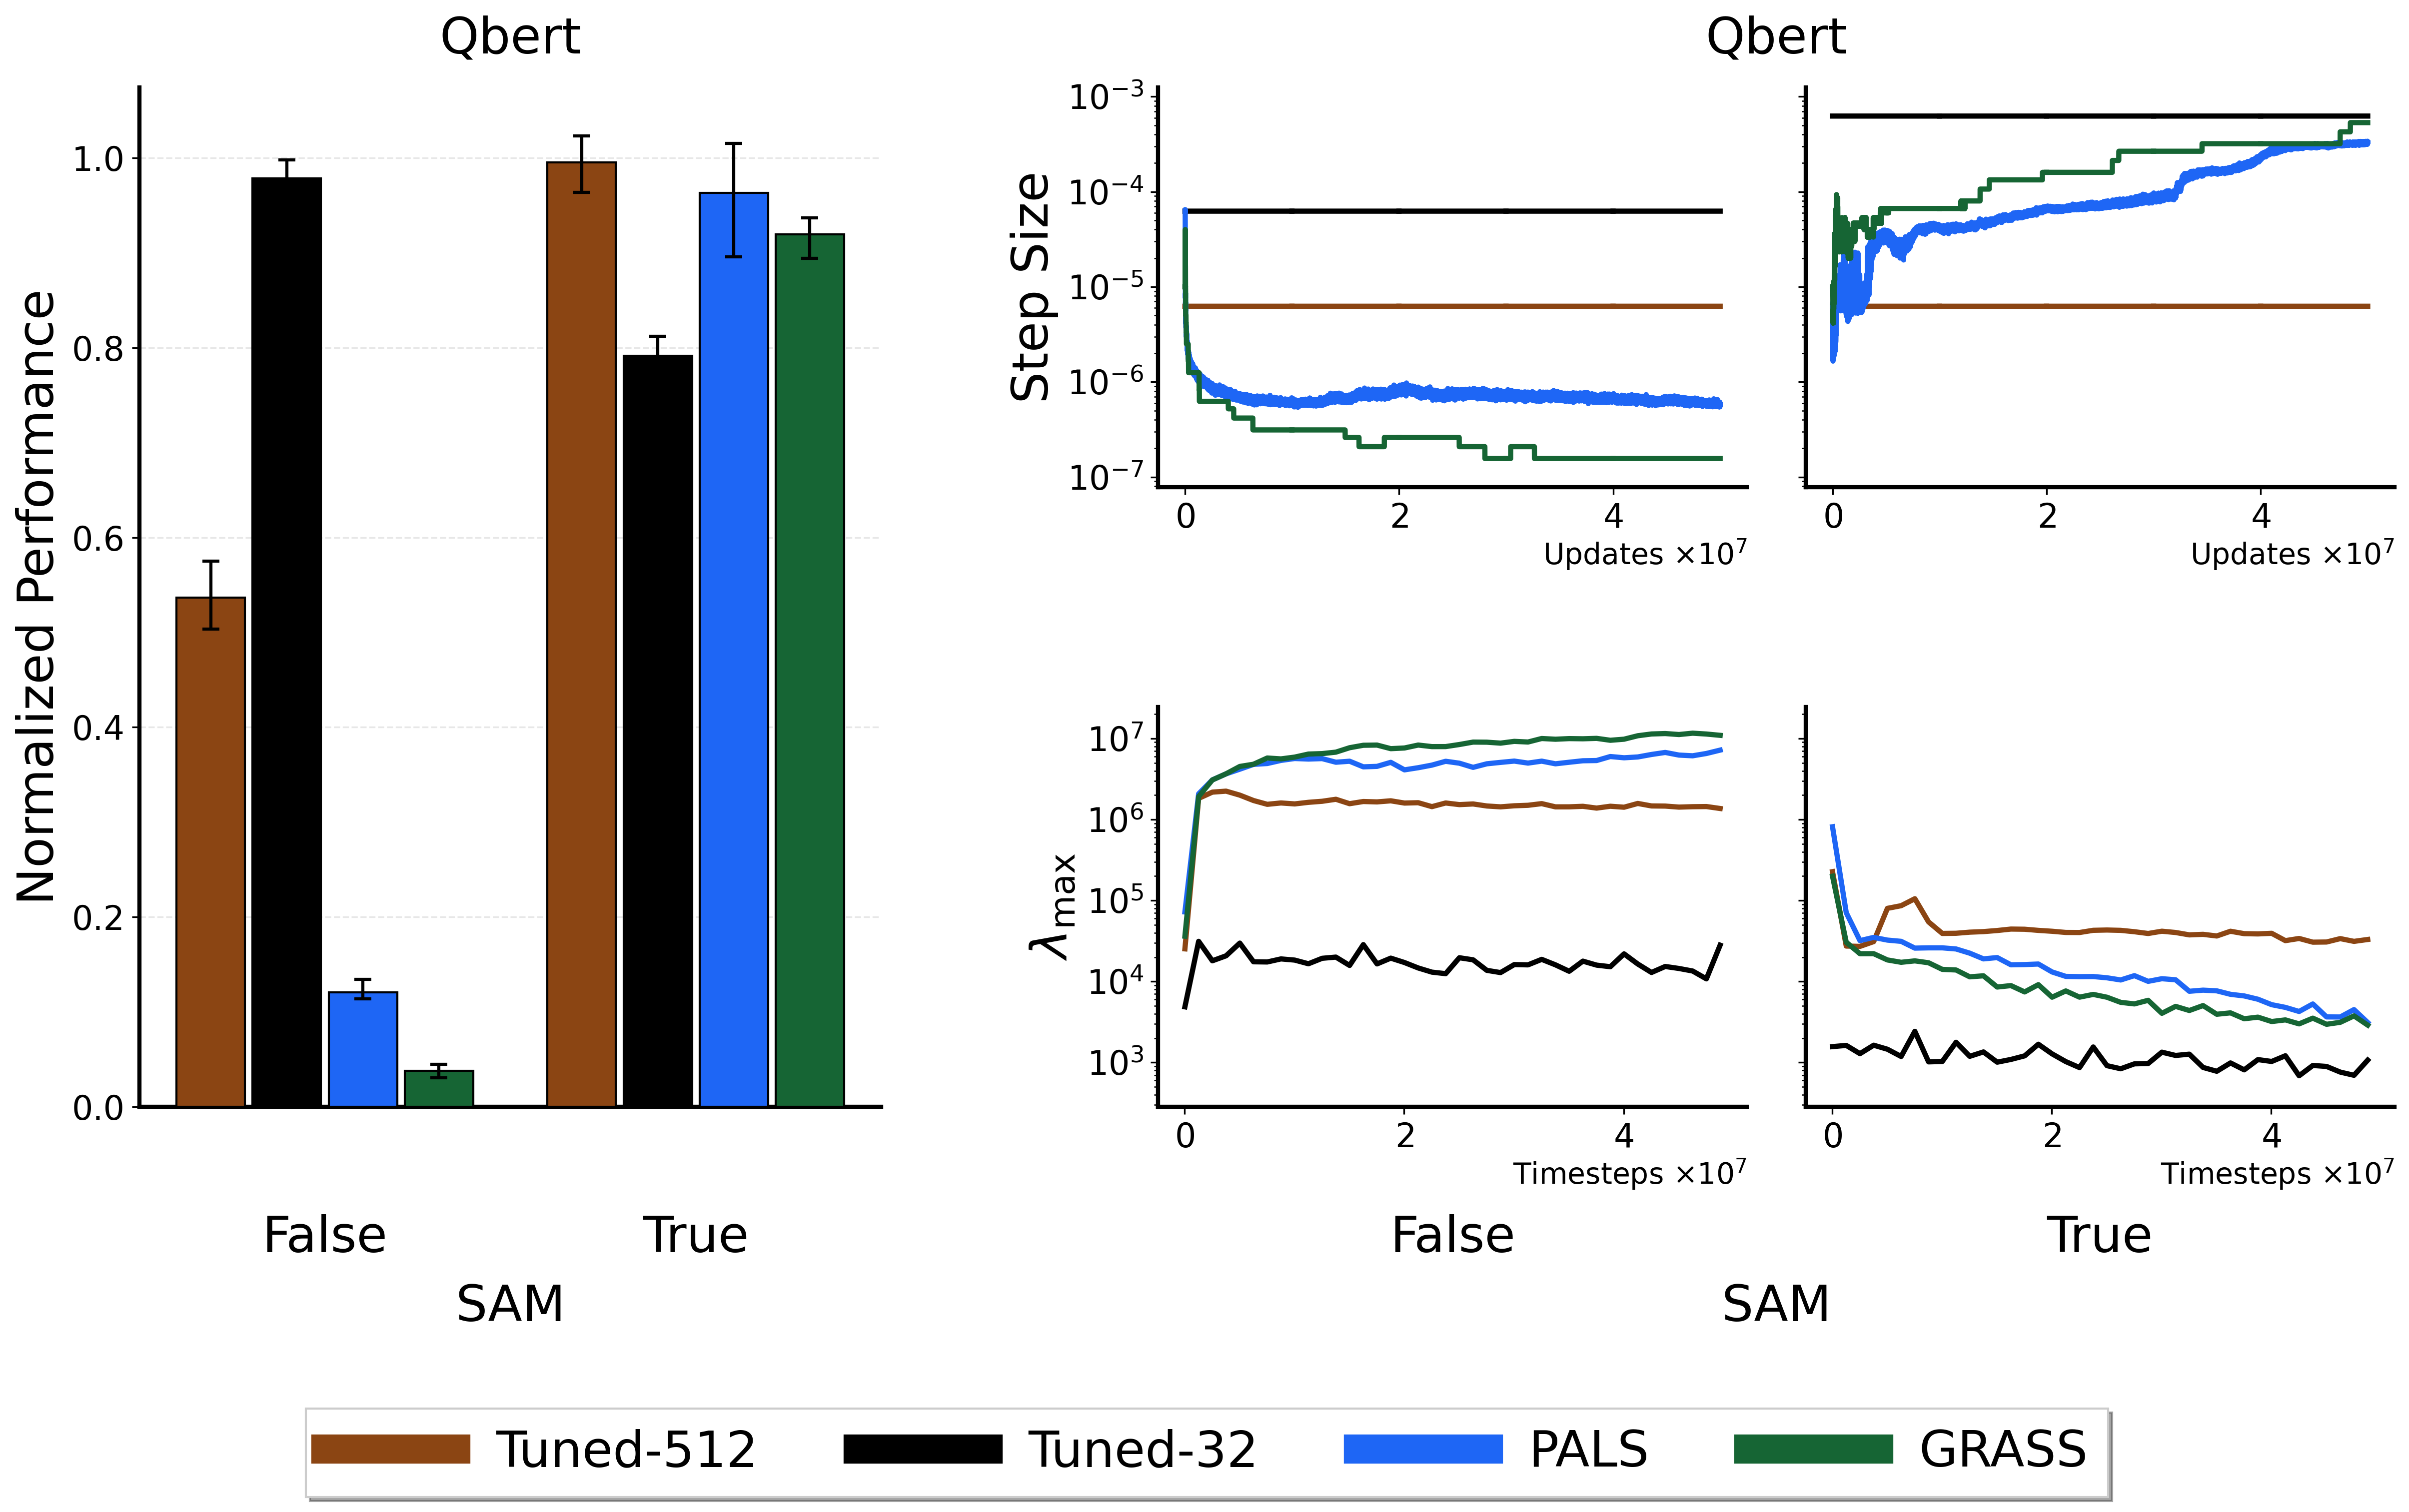
\includegraphics[width=\textwidth]{figures/thesis/ablations/1_sam/sam_qbert_step_sharpness.png}
    \caption[DQN with and without SAM in Qbert]{\textbf{(a) Left:} Normalized performance and \textbf{(b) Right:} Step size and preconditioned sharpness, with and without SAM in Qbert. When using SAM, chosen step sizes were larger and sharpness decreased to more closely match the fixed step size baselines.}
    \label{fig:sam_qbert}
\end{figure}
Figure~\ref{fig:sam_qbert}(a) compares the performance of PALS and GRASS in Qbert with and without SAM, an environment in which both methods previously failed to learn. When using SAM, the adaptive methods were competitive with the tuned baselines, whose performance was also slightly improved. Figure~\ref{fig:sam_qbert}(b) shows that when using SAM the chosen step sizes were much larger, within an order of magnitude below or above the tuned baseline. As a result, we found that sharpness also decreased and closely matched that of Tuned-32 for both the adaptive methods and Tuned-512. To confirm the effectiveness of SAM in this environment, Figure~\ref{fig:sam_qbert_stepsize_loss} examines the loss along the update direction for a single update with PALS in Qbert.
We found the loss landscape to indeed be smoother when using SAM, allowing PALS to accept a step size with a larger resulting displacement.

\begin{figure}[htbp]
    \centering
    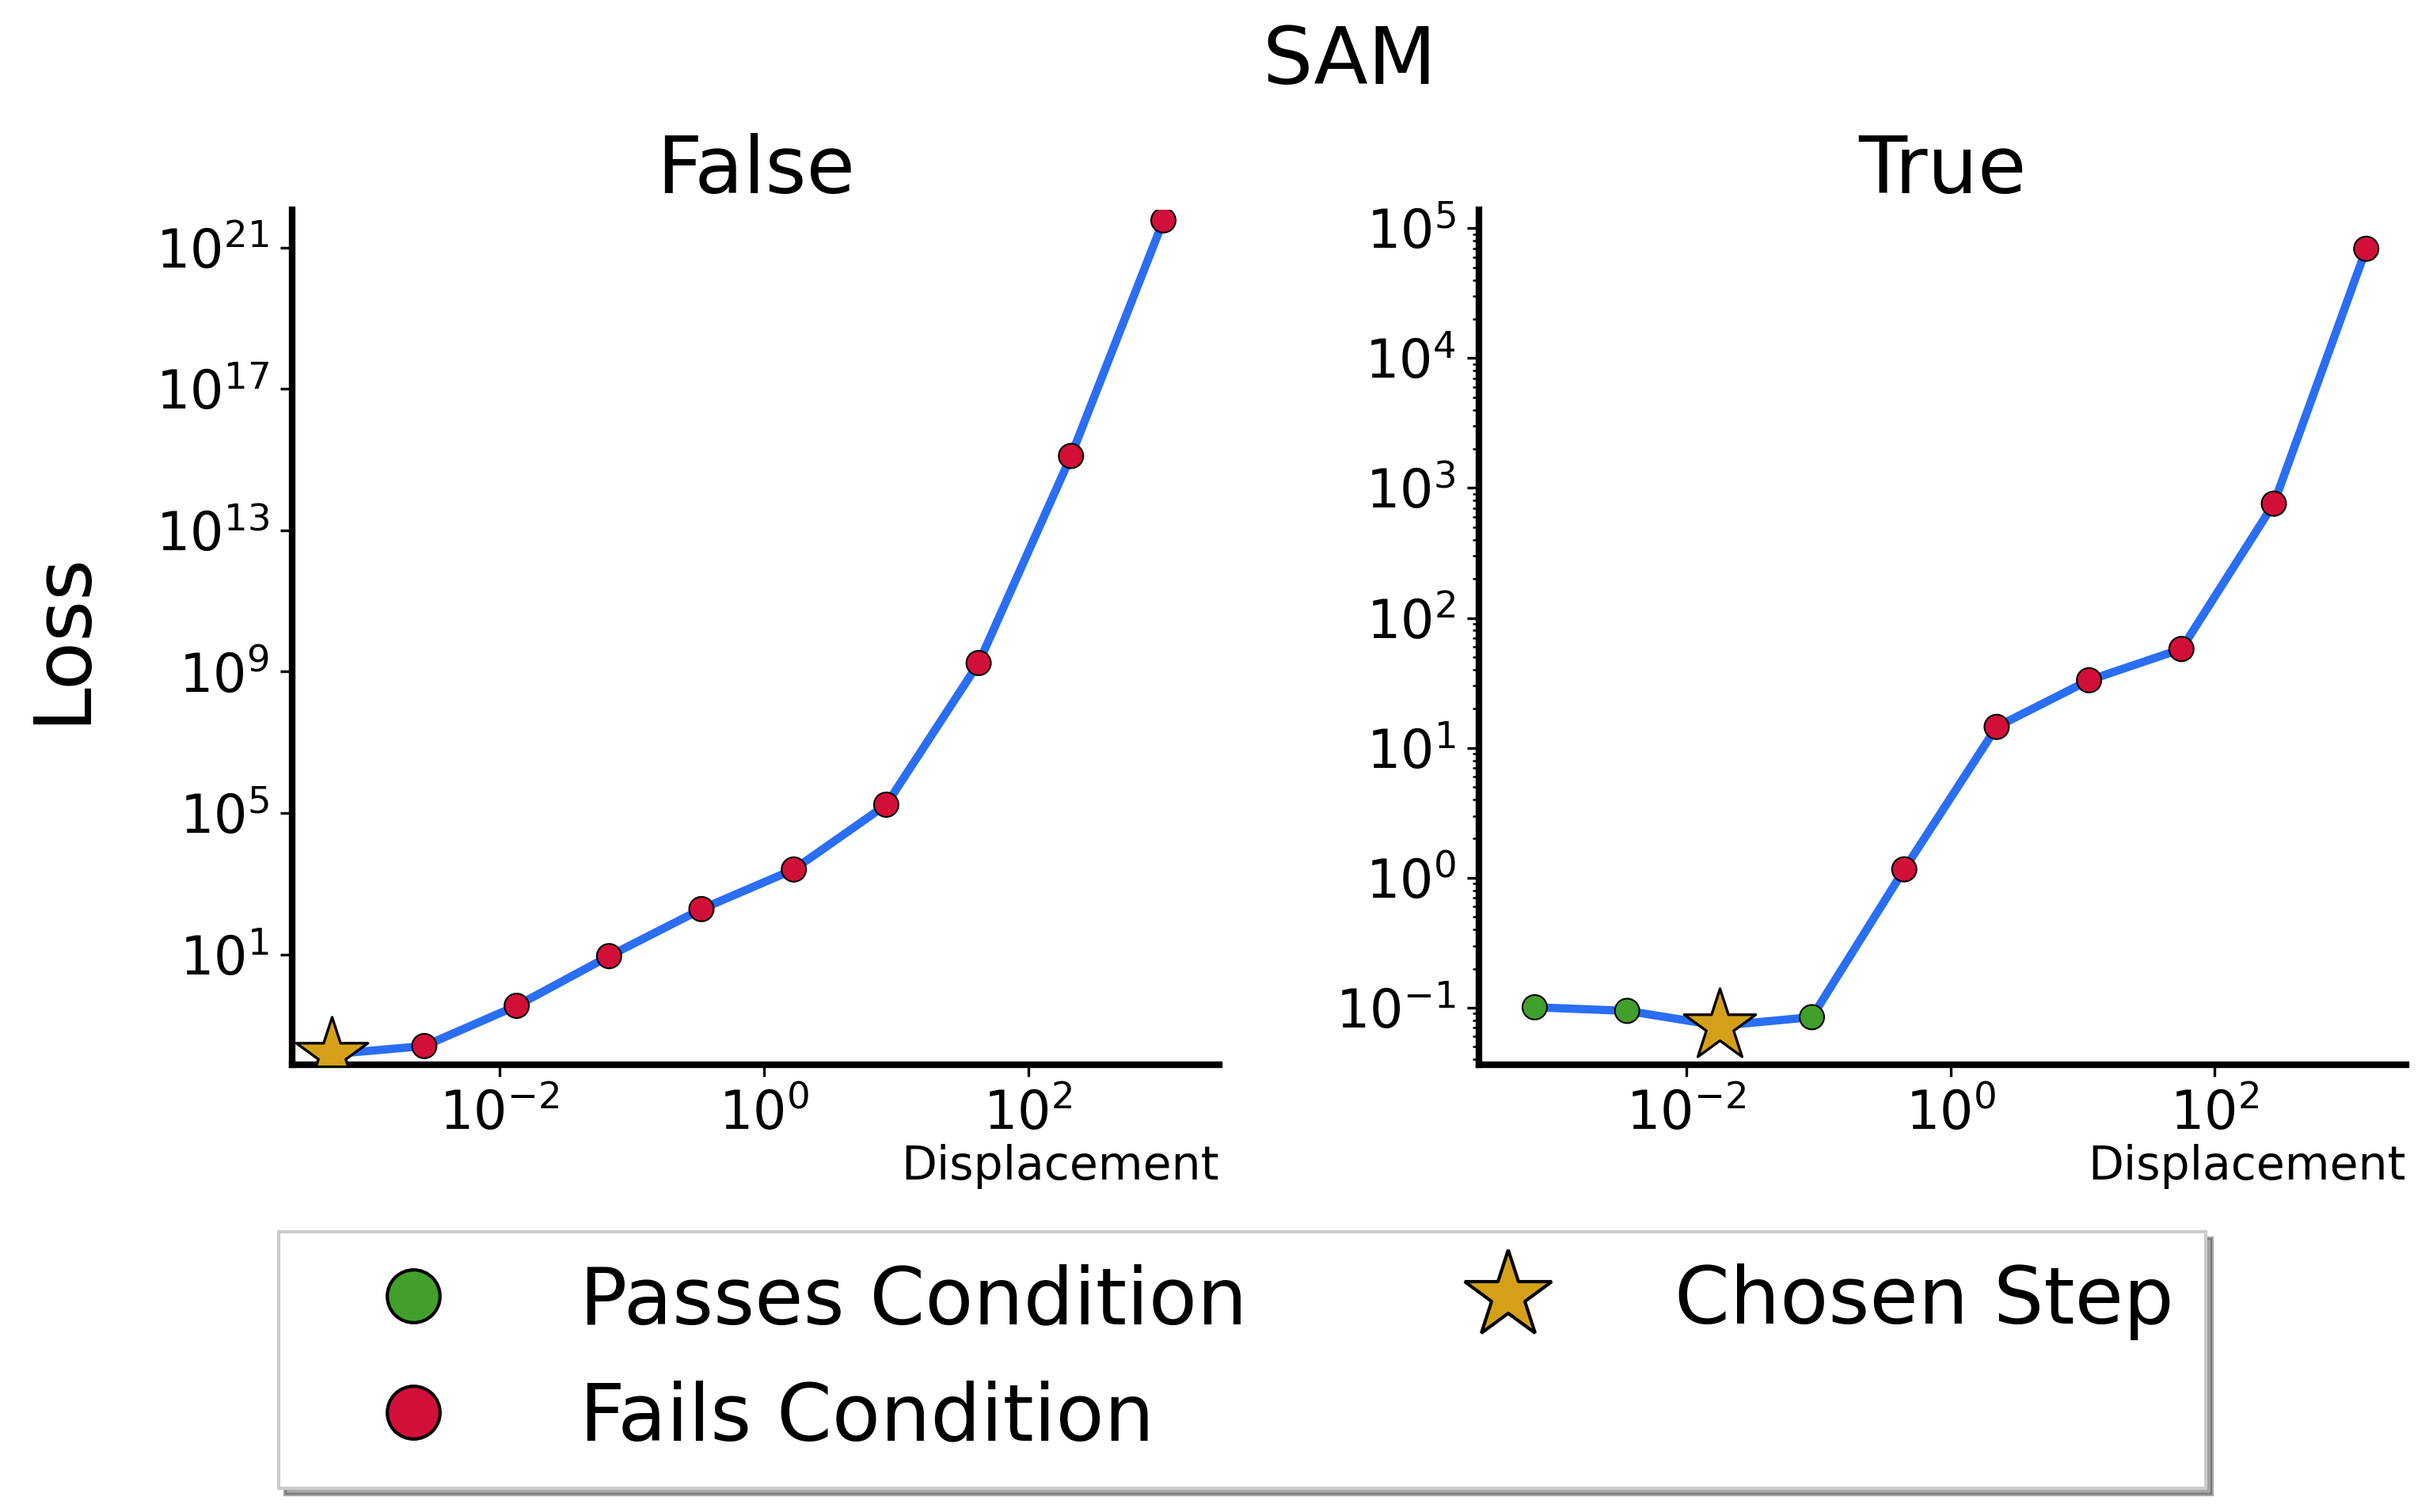
\includegraphics[width=\textwidth]{figures/thesis/ablations/1_sam/sam_qbert_stepsize_loss.png}
    \caption[Loss landscape for SAM in Qbert.]{Loss landscape approximation along the update direction for a single PALS update in Qbert, with and without SAM. The loss was smoother when using SAM, allowing PALS to accept a step size with a larger resulting displacement.}
    \label{fig:sam_qbert_stepsize_loss}
\end{figure}

The steady increase in step size when using SAM for both methods is concerning, as it resembles the pattern of the failure modes observed in Section~\ref{sec:dqn_results}, where some methods suffered from performance degradation over the course of the run.
Indeed, examining Figure~\ref{fig:sam_atari5}(a), we found that while performance across the Atari-5 was improved for PALS and Tuned-512, performance for GRASS was unchanged due to worsened behavior in some environments, as shown in Battle Zone in Figure~\ref{fig:sam_atari5}(b).
\begin{figure}[htbp]
    \centering
    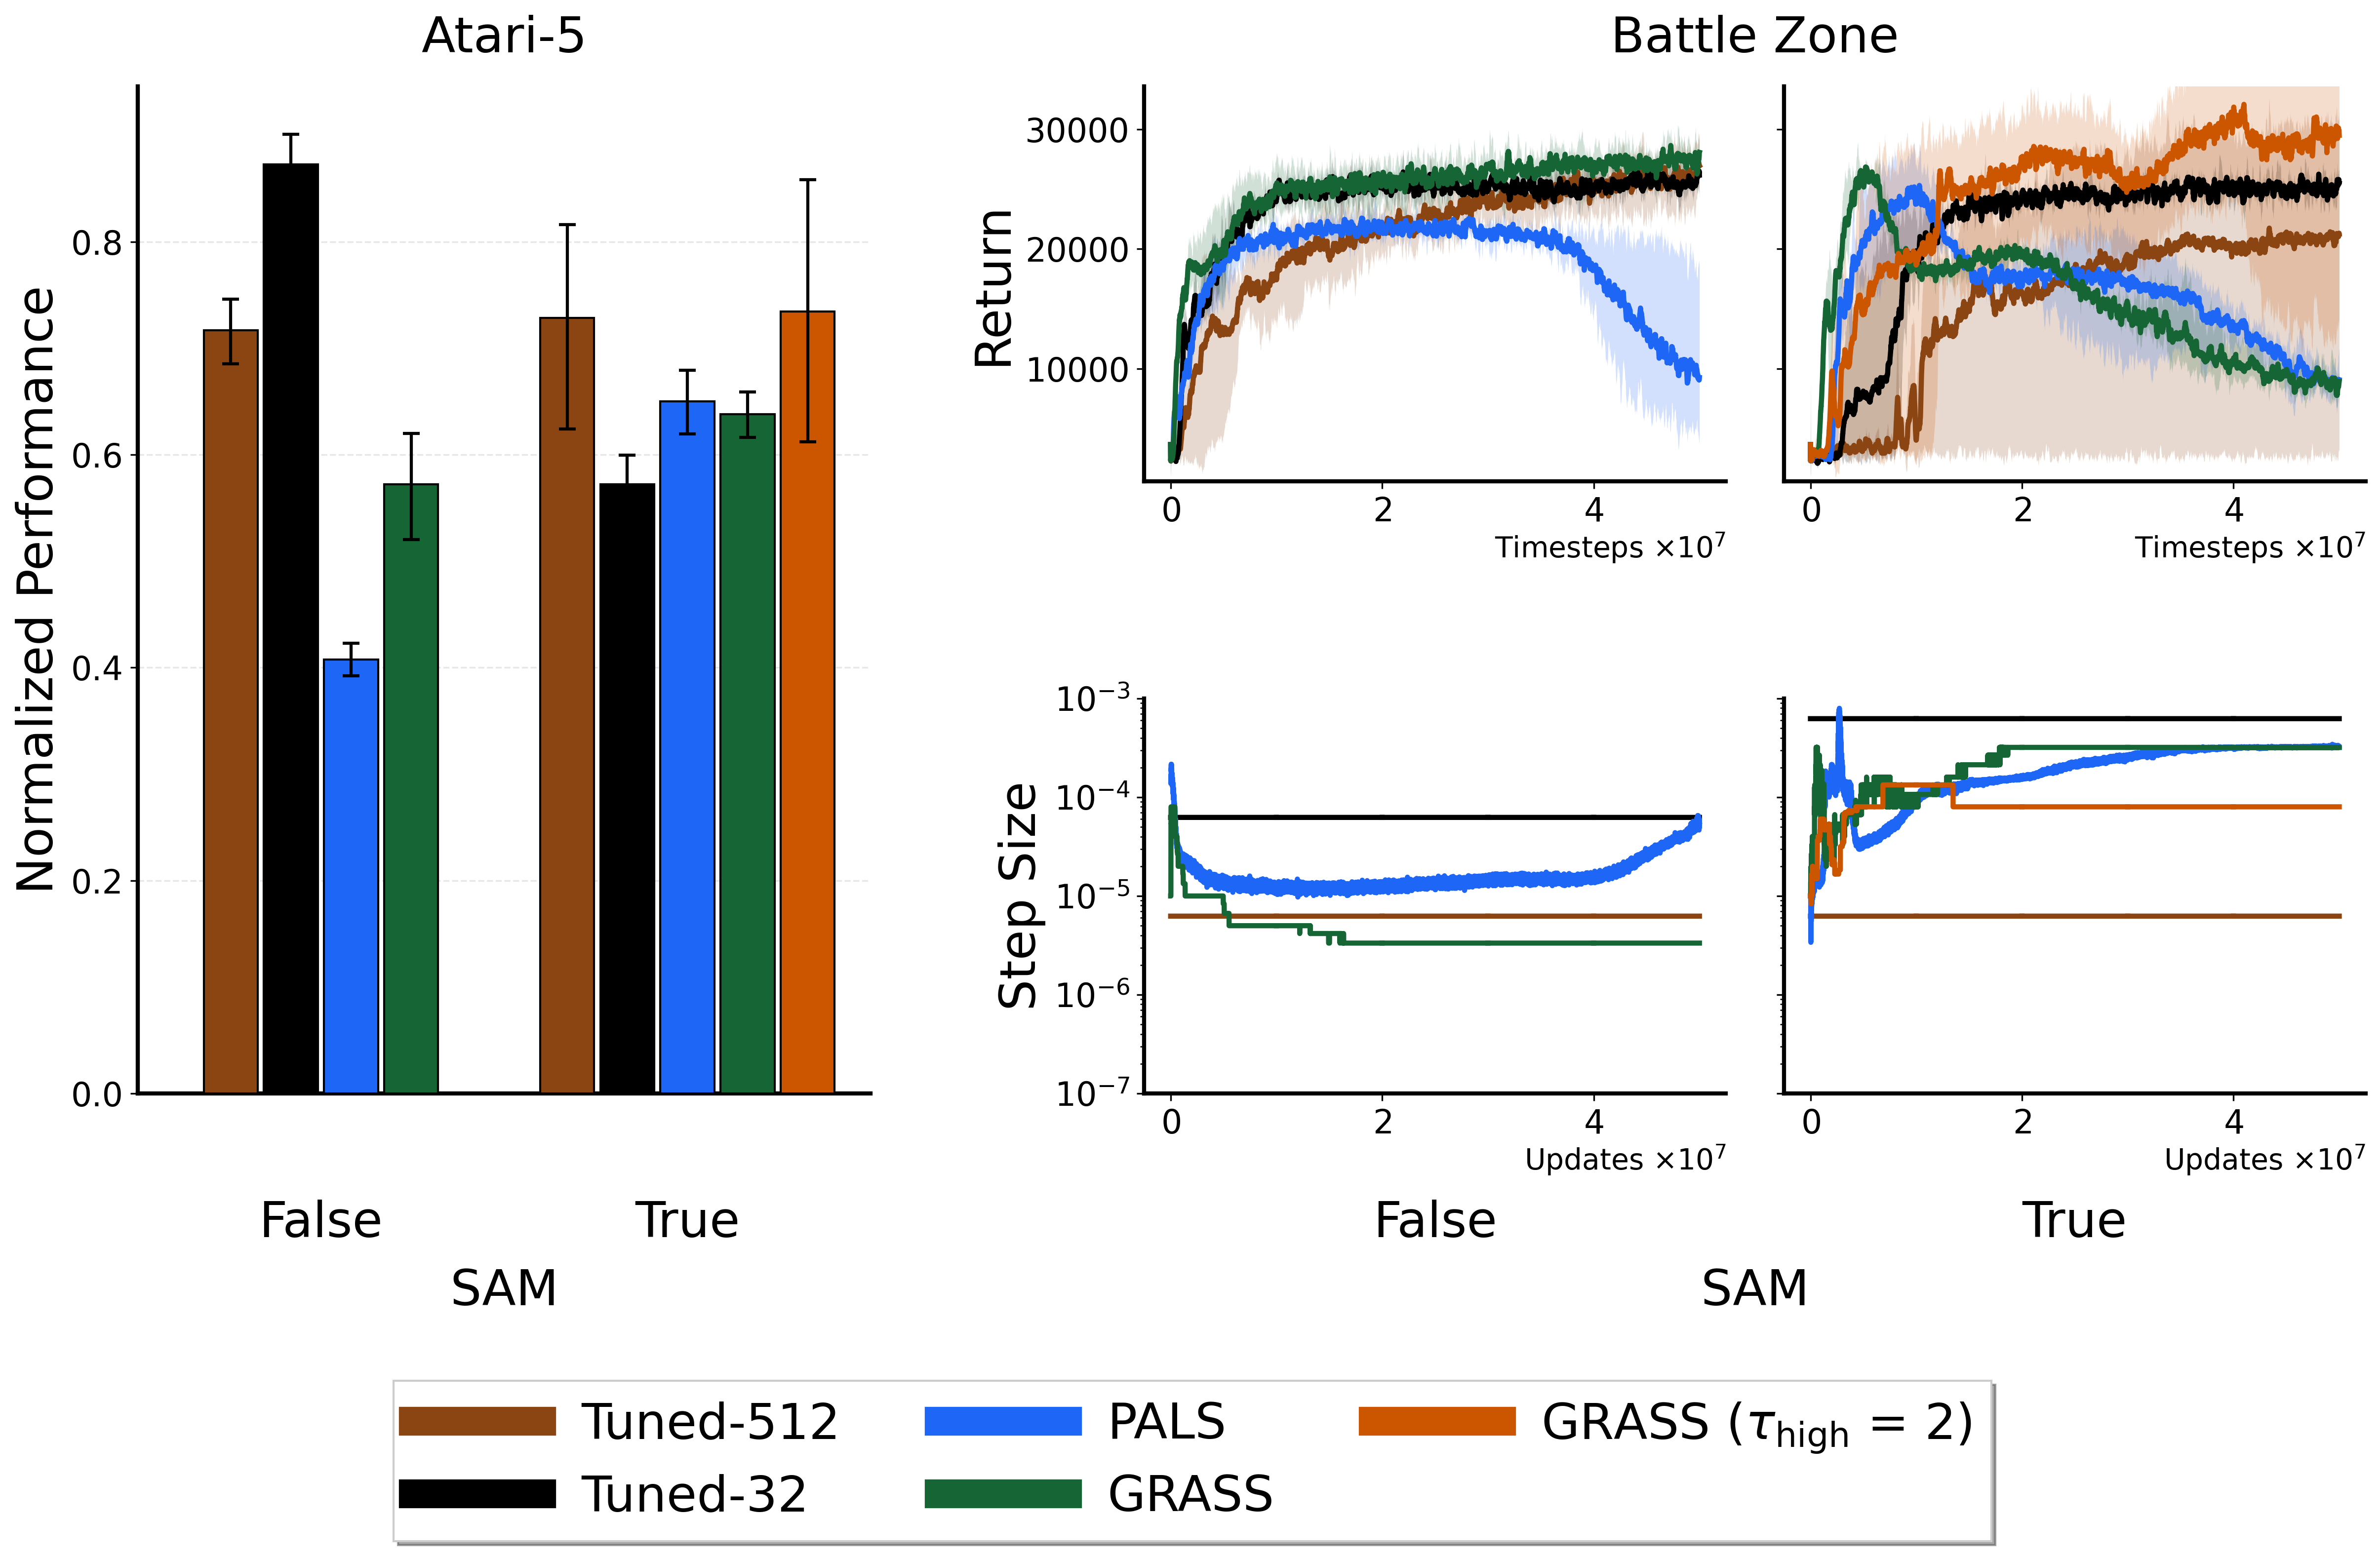
\includegraphics[width=\textwidth]{figures/thesis/ablations/1_sam/sam_atari5_return_step.png}
    \caption[SAM vs.\ no SAM on Atari-5: return and step size.]{\textbf{(a) Left:} Normalized performance and step size, and \textbf{(b) Right:} return and step size in Battle Zone, for DQN with Adam on the Atari-5, with and without SAM. Performance was improved for PALS and Tuned-512, while GRASS was unchanged due to worsened behavior in Battle Zone.}
    \label{fig:sam_atari5}
\end{figure}
In this environment, we observed the steadily increasing step size and corresponding performance degradation seen with other globalization strategies in Section~\ref{sec:dqn_results}. This finding suggests that selecting step size based on the SAM objective can lead to aggressively large steps for the true objective. To address this issue with GRASS, one can increase the growth threshold $T_{\text{hi}}$ in the gain-ratio, as shown in Figure~\ref{fig:sam_atari5}(a), which improved performance by making the method more conservative. However, in practice we found that this change was overfit to Atari, harming performance in classic control.

The improved performance of Tuned-512 with SAM supports the view that the loss of the implicit regularization afforded by small batch size is harmful with DQN in Atari. Conversely, Tuned-32 failed with SAM, \todo{Note for Adam: Think this could be because I didn't retune with SAM, currently running this before i say anything further}

\chapter{Conclusion and Future Work} \label{sec: conclusion}
The performance of deep RL algorithms is notoriously sensitive to hyperparameters. Step size, which serves as the primary mechanism for controlling the magnitude of an update, is particularly difficult to set for each new environment. Popular hyperparameter tuning methods such as grid-search are typically only tractable with access to a simulator, which is not available for many real-world settings such as industrial control. This motivated our examination of line search and trust region methods to autonomously select step size for deep RL algorithms while learning online.

In this thesis we introduced two first-order methods for adaptive step size and examined their effectiveness in deep RL. PALS evaluates many candidate step sizes in parallel rather than using the traditional backtracking approach. This removes the linear complexity of backtracking and allows for a selection criterion based on the greatest reduction in the objective among those satisfying the Armijo condition. GRASS uses the gain-ratio heuristic of trust region methods to iteratively adjust the step size directly, rather than adapting the radius of a strict trust region around the current parameters. This effectively preserves the magnitude of the update vector rather than normalizing it. We also introduced two modifications intended to stabilize the chosen step size in the high-variance regime of online RL: an exponential moving average over the step sizes accepted by a line search and the median of the gain ratio over a window of updates, both of which can be applied with any line search or trust region method, respectively. We identified an effective approach for combining globalization strategies with the Adam optimizer in deep RL by dropping the momentum term from step size selection while still updating along the momentum direction. Lastly, we showed that Sharpness Aware Minimization can prevent these methods from selecting pathologically conservative step sizes in some environments, at the cost of overly aggressive step size in others. 

We evaluated the use of these methods for PPO and DQN with the Adam optimizer, comparing PALS and GRASS against traditional line search and trust region methods as well as tuned fixed step sizes and schedules with varying batch size. All the examined adaptive methods performed roughly equally well with both algorithms in classic control, matching the tuned baselines and demonstrating that globalization strategies can serve as an effective means of automatic step size selection in deep RL. Results in the more complex environments were considerably more nuanced. With DQN in the Atari-5, GRASS greatly outperformed all the standard line search and trust region methods, with PALS ranking second by a substantial margin. However, neither method matched the tuned baseline at either of the examined batch sizes in these environments. We observed that in Atari globalization strategies were susceptible to both highly inflated value estimates and overly conservative step sizes depending on the environment, and identified sharpness aware minimization as a promising fix for the later issue. With PPO in Brax, GRASS and PALS were competitive with the tuned baselines across the suite. The superior performance of GRASS relative to the trust region methods in these environments indicated that preserving the magnitude of the update, rather than using only its direction, was especially useful. Lastly, ablations revealed that large batch size and removing momentum from step size selection were both essential for good performance when using these adaptive methods with DQN and PPO. 

These results indicate that globalization strategies are a promising mechanism for automatic step size selection in deep RL, but they are not without limitations. Of particular note was the strong performance of GRASS relative to the tuned fixed step size baselines at fraction of the computational cost of line search. However, the effectiveness of these methods can still vary greatly depending on the algorithm and environment. Poor performance in the ALE exposed several key failure modes of these methods when applied with DQN. It may be that these methods require even larger batch size in this environment to prevent selecting overly aggressive steps that, while productive for the batch loss, result in higher variance updates that can destabilize progress on the true loss. % opus todo: make note of how this relates to the fact that the interpolation condition used in the painless sgd paper that introduced stochastic line search may not hold
Additionally, while our results with SAM showed that smoothing the loss landscape can prevent overly conservative step size, this can also produce large steps that lead to performance degradation. Further work is needed to identify a more robust approach for this issue, though larger batch size may be a promising fix as well. Lastly, DQN is known to suffer from many instabilities during training such as overestimation bias \tocite{citation}, which have been addressed by more sophisticated algorithms like Double DQN \tocite{ddqn} and RAINBOW \tocite{rainbow}. Future work could examine if the more stable targets and potentially better conditioned loss provided by these algorithms may resolve the observed failure cases for globalization strategies.

A key limitation of this work is that popular deep RL benchmarks fail to demonstrate the need for adaptive step size methods for two distinct reasons. First, these environments are fully observable and do not capture the non-stationarity present in the real-world that motivates the need for methods capable of adapting their hyperparameters during learning. % opus todo: make not a run on and more clear
Second, the best tuned step size is the same across all environments in both the Atari-5 and Brax suites, allowing a single fixed step size to perform well across all the examined MDPs. This does not reflect the diversity of real-world applications \todo{citation}, where a single fixed step size is unlikely to achieve the best performance in every application of a given algorithm. Non-stationary environments that require adapting step size over time to attain good performance, similar to the bit-flipping problem from supervised learning \tocite{sutton idbd}, or stationary MDPs where the best fixed step size varies for each environment would provide more suitable testbeds for these methods. 

\renewcommand{\bibname}{References}
\bibliography{ref}
\bibliographystyle{IEEEtran}

\appendix
\chapter{Pseudocode for Adaptive Step Size Methods} \label{app_algo_pseudocode}
Algorithm~\ref{alg:armijo-ema} gives the backtracking Armijo line search with an EMA on the chosen step size introduced in Chapter~\ref{sec: methods}. 

\begin{algorithm}[H]
    \caption{Backtracking Armijo Line Search with EMA}
    \label{alg:armijo-ema}
    \begin{algorithmic}[1]
        \State \textbf{Input:} (possibly stochastic) loss function $f$, initial point $\xAt{0}$, sufficient decrease constant $c \in (0, 1)$, initial step size $\stepSizeInit > 0$, contraction factor $\beta \in (0, 1)$, backtracking steps $B \in \mathbb{N}$, EMA decay rate $\zeta \in (0, 1)$
        \State Initialize iteration counter $k \gets 0$, EMA step size $\bar{\stepSize}_{-1} \gets \stepSizeInit$
        \For{each update}
            \State Compute descent direction $\updateAt{k}$ \Comment{e.g., $\updateAt{k} = -\nabla f_k(\xAt{k})$}
            \State $i \gets 0$, accepted $\gets$ false
            \While{$i \le B$ and \textbf{not} accepted}
                \If{$f_k(\xAt{k} + \stepSizeInit \beta^i \updateAt{k}) \le f_k(\xAt{k}) + c\, \stepSizeInit \beta^i \inner{\nabla f_k(\xAt{k})}{\updateAt{k}}$}
                    \State $\stepSizeAt{k}^* \gets \stepSizeInit \beta^i$, accepted $\gets$ true
                \Else
                    \State $i \gets i + 1$
                \EndIf
            \EndWhile
            \If{\textbf{not} accepted}
                \State $\stepSizeAt{k}^* \gets \stepSizeInit \beta^B$ \Comment{fallback if the Armijo condition is not met}
            \EndIf
            \State $\bar{\stepSize}_k \gets \zeta \bar{\stepSize}_{k-1} + (1 - \zeta) \stepSizeAt{k}^*$ \Comment{EMA over the chosen step size}
            \State Update point: $\xAt{k+1} \gets \xAt{k} + \bar{\stepSize}_k \updateAt{k}$
            \State Increment counter: $k \gets k + 1$
        \EndFor
    \end{algorithmic}
\end{algorithm}

\chapter{Environment and Implementation Details}

\section{Classic Control Implementation Differences} \label{app_classic_control_diffs}
The Acrobot, CartPole, and MountainCar environments used in this work are implemented as edited versions of the corresponding \texttt{gymnax} \tocite{gymnax} environments. One change is applied uniformly across all three environments, while the other change is specific to MountainCar. 

\paragraph{Change applied to all three environments.}
\begin{itemize}
    \item \textbf{Proper episode cutoff termination.} Reaching the maximum episode length is now reported as a truncation signal, which is kept separate from the terminal signal and used to bootstrap value estimates. These transitions are conflated with true termination in the underlying \texttt{gymnax} implementations.
\end{itemize}

\paragraph{MountainCar.} In addition to the change above, MountainCar uses:
\begin{itemize}
    \item \textbf{The classic MountainCar termination condition and reward}, rather than those of \texttt{gymnax}'s continuous-action MountainCar: the episode terminates only when the goal position is reached, and the reward is $-1$ per timestep until termination.
    \item \textbf{Gym-based goal position and power} of $(0.45, 0.0015)$, rather than the classic values of $(0.5, 0.001)$ used by \cite{sutton1998introduction}. Here the environment follows the modern Gym convention rather than the original Sutton and Barto dynamics, chosen for consistency with the widely used Gym benchmark values.
\end{itemize}


\section{Arcade Learning Environment Configuration} \label{app_ale_params}
All Atari-5 experiments use \texttt{ale\_py}'s vectorized ALE interface, \texttt{AtariVectorEnv}, with a single environment instance (\texttt{num\_envs = 1}). Table~\ref{tab:ale_params} lists every configurable parameter of \texttt{AtariVectorEnv} and the value used in this work.

\begin{table}[htbp]
\centering
\small
\setlength{\tabcolsep}{6pt}
\renewcommand{\arraystretch}{1.2}
\begin{tabular}{@{}l l@{}}
\toprule
Parameter & Value Used \\
\midrule
\texttt{game} & per Atari-5 game (see caption) \\
\texttt{num\_envs} & 1 \\
\texttt{frameskip} & 4 \\
\texttt{grayscale} & True \\
\texttt{stack\_num} & 4 \\
\texttt{img\_height} & 84 \\
\texttt{img\_width} & 84 \\
\texttt{maxpool} & True \\
\texttt{reward\_clipping} & True \\
\texttt{noop\_max} & 0 \\
\texttt{use\_fire\_reset} & False \\
\texttt{episodic\_life} & False \\
\texttt{life\_loss\_info} & False \\
\texttt{max\_num\_frames\_per\_episode} & 108{,}000 (27{,}000 agent steps at a frameskip of 4) \\
\texttt{repeat\_action\_probability} & 0.25 \\
\texttt{full\_action\_space} & False (minimal, per-game action set) \\
\texttt{continuous} & False \\
\texttt{continuous\_action\_threshold} & 0.5 \\
\texttt{batch\_size} & 0 (i.e.\ \texttt{num\_envs}) \\
\texttt{autoreset\_mode} & \texttt{SAME\_STEP} \\
\texttt{num\_threads} & 0 (auto) \\
\texttt{thread\_affinity\_offset} & $-1$ (no affinity) \\
\bottomrule
\end{tabular}
\caption[\texttt{AtariVectorEnv} configuration used for all Atari-5 experiments.]{\texttt{AtariVectorEnv} configuration used for all Atari-5 experiments. The five games examined are battle\_zone, double\_dunk, name\_this\_game, phoenix, and qbert.}
\label{tab:ale_params}
\end{table}

\chapter{Algorithm and Optimizer Hyperparameters}

\section{DQN and PPO Hyperparameters} \label{app_hyperparams}
Tables~\ref{tab:dqn_hypers} and~\ref{tab:ppo_hypers} report the DQN and PPO algorithm, network, and Adam optimizer hyperparameters, respectively, used for each environment suite examined in this work. These settings are shared by all methods, both adaptive and fixed step size. Hyperparameters belonging to the step size selection method itself rather than to the underlying RL algorithm (such as $K$, $T_{\text{lo}}$, $T_{\text{hi}}$, $\alpha_{\text{shrink}}$, $\alpha_{\text{grow}}$, $B$, and $\beta$) are given in Section~\ref{sec:algorithms}. For each algorithm we report the batch size used by the adaptive step size methods as well as the batch sizes used by the tuned fixed step size baselines described in Section~\ref{sec:algorithms}.

\begin{table}[htbp]
\centering
\small
\setlength{\tabcolsep}{6pt}
\renewcommand{\arraystretch}{1.2}
\begin{tabular}{@{}l l l@{}}
\toprule
Hyperparameter & Classic Control & Atari-5 \\
\midrule
Environment timesteps & 150{,}000 & 50{,}000{,}000 \\
Discount factor $\gamma$ & 0.99 & 0.99 \\
Network & \makecell[l]{MLP: 2 hidden layers \\ (128, 80), ReLU} & \makecell[l]{Nature CNN \\ conv 32, $8{\times}8$, stride 4 \\ conv 64, $4{\times}4$, stride 2 \\ conv 64, $3{\times}3$, stride 1 \\ FC 512; ReLU} \\
Adaptive-method batch size & 1024 & 512 \\
Fixed-baseline batch sizes & 32, 1024 & 32, 512 \\
Replay buffer capacity & 10{,}000 & 1{,}000{,}000 \\
Steps before learning & 10{,}000 & 20{,}000 \\
Training interval & 4 & 4 \\
Target update interval & 600 & 8{,}000 \\
Target update rate & 1.0 & 1.0 \\
Exploration $\epsilon$ (start $\to$ finish) & $1.0 \to 0.05$ & $1.0 \to 0.01$ \\
$\epsilon$ anneal steps & 15{,}000 & 250{,}000 \\
Reward clipping & none & $\operatorname{sign}(\cdot)$ \\
Adam $\beta_1$ & $0.9$ & $0.9$ \\
Adam $\beta_2$ & $0.999$ & $0.999$ \\
Adam $\epsilon$ & $0.00000001$ & $0.00015$ \\
\bottomrule
\end{tabular}
\caption{DQN algorithm and network hyperparameters.}
\label{tab:dqn_hypers}
\end{table}

\begin{table}[htbp]
\centering
\small
\setlength{\tabcolsep}{6pt}
\renewcommand{\arraystretch}{1.2}
\begin{tabular}{@{}l l l@{}}
\toprule
Hyperparameter & Classic Control & Brax \\
\midrule
Environment timesteps & 150{,}000 & 3{,}000{,}000 \\
Discount factor $\gamma$ & \multicolumn{2}{c}{0.99} \\
Network (actor \& critic) & \multicolumn{2}{c}{MLP: 2 hidden layers (64, 64), tanh} \\
Adaptive-method batch size & \multicolumn{2}{c}{1024} \\
Fixed-baseline batch sizes & \multicolumn{2}{c}{64, 1024} \\
Rollout length (steps) & \multicolumn{2}{c}{2048} \\
Update epochs & \multicolumn{2}{c}{10} \\
GAE $\lambda$ & \multicolumn{2}{c}{0.95} \\
Clip parameter $\epsilon$ & \multicolumn{2}{c}{0.2} \\
Entropy coefficient & \multicolumn{2}{c}{0.0} \\
Max gradient norm & \multicolumn{2}{c}{0.5} \\
Observation normalization & \multicolumn{2}{c}{on} \\
Reward normalization & \multicolumn{2}{c}{on} \\
Fixed step size schedule & \multicolumn{2}{c}{linear decay} \\
Adam $\beta_1$ & $0.9$ & $0.9$ \\
Adam $\beta_2$ & $0.999$ & $0.999$ \\
Adam $\epsilon$ & $0.00001$ & $0.00001$ \\
\bottomrule
\end{tabular}
\caption[PPO algorithm and network hyperparameters.]{PPO algorithm and network hyperparameters. All settings other than the environment timestep budget are shared across the two suites.}
\label{tab:ppo_hypers}
\end{table}

\section{Fixed Step Size Tuning Ranges} \label{app_tuning_ranges}
For each environment suite, algorithm, and optimizer, we perform a grid search over the range of candidate fixed step sizes given in Table~\ref{tab:tuning_ranges} to obtain the \textit{Tuned N} baselines described in Section~\ref{sec:algorithms}, where $N$ denotes the batch size used. Table~\ref{tab:tuned_n} reports the selected fixed step size for each environment suite, algorithm, and optimizer. In every setting the selected step size was identical across the batch sizes examined, so a single value is reported per row.

\begin{table}[htbp]
\centering
\small
\setlength{\tabcolsep}{6pt}
\renewcommand{\arraystretch}{1.2}
\begin{tabular}{@{}l l l@{}}
\toprule
Env. Suite & Algorithm & Grid Search Range \\
\midrule
Classic Control & DQN & $1\mathrm{e}{-5}$ to $1\mathrm{e}{-1}$ \\
Atari-5 & DQN & $6.25\mathrm{e}{-6}$ to $6.25\mathrm{e}{-1}$ \\
Classic Control & PPO & $3\mathrm{e}{-5}$ to $3\mathrm{e}{-1}$ \\
Brax & PPO & $3\mathrm{e}{-5}$ to $3\mathrm{e}{-1}$ \\
\bottomrule
\end{tabular}
\caption{Grid search range for fixed step size tuning, by environment suite and algorithm.}
\label{tab:tuning_ranges}
\end{table}

\begin{table}[htbp]
\centering
\small
\setlength{\tabcolsep}{6pt}
\renewcommand{\arraystretch}{1.2}
\begin{tabular}{@{}l l l l l@{}}
\toprule
Env. Suite & Algorithm & Optimizer & Batch Sizes & Step Size \\
\midrule
Classic Control & DQN & Adam & 32, 1024 & $1\mathrm{e}{-3}$ \\
Atari-5 & DQN & Adam & 32, 512 & $6.25\mathrm{e}{-5}$ \\
Classic Control & PPO & Adam & 64, 1024 & $3\mathrm{e}{-3}$ \\
Brax & PPO & Adam & 64, 1024 & $3\mathrm{e}{-4}$ \\
\bottomrule
\end{tabular}
\caption[Selected fixed step size for each environment suite, algorithm, and optimizer.]{Selected fixed step size for each environment suite, algorithm, and optimizer. The step size was identical across the batch sizes examined in every setting. Atari-5 DQN was run only with Adam.}
\label{tab:tuned_n}
\end{table}

\end{document}